\documentclass[twocolumn,a4paper]{article}
\usepackage{fontspec}   %加這個就可以設定字體
\usepackage{xeCJK}       %讓中英文字體分開設置
\usepackage{indentfirst}
\usepackage{listings}
\usepackage[newfloat]{minted}
\usepackage{float}
\usepackage{graphicx}
\usepackage{caption}
\usepackage{fancyhdr}
\usepackage{hyperref}
\usepackage{amsmath}
\usepackage{multirow}
\usepackage[dvipsnames]{xcolor}
\usepackage{graphicx}
\usepackage{tabularx}
\usepackage{booktabs}
\usepackage{caption}
\usepackage{subcaption}
\usepackage{pifont}
\usepackage{amssymb}


\usepackage{pdftexcmds}
\usepackage{catchfile}
\usepackage{ifluatex}
\usepackage{ifplatform}

\usepackage[breakable, listings, skins, minted]{tcolorbox}
\usepackage{etoolbox}
\setminted{fontsize=\footnotesize}
\renewtcblisting{minted}{%
    listing engine=minted,
    minted language=python,
    listing only,
    breakable,
    enhanced,
    minted options = {
        linenos, 
        breaklines=true, 
        breakbefore=., 
        % fontsize=\footnotesize, 
        numbersep=2mm
    },
    overlay={%
        \begin{tcbclipinterior}
            \fill[gray!25] (frame.south west) rectangle ([xshift=4mm]frame.north west);
        \end{tcbclipinterior}
    }   
}

\usepackage[
top=1.5cm,
bottom=0.75cm,
left=1.5cm,
right=1.5cm,
includehead,includefoot,
heightrounded, % to avoid spurious underfull messages
]{geometry} 

\newenvironment{code}{\captionsetup{type=listing}}{}
\SetupFloatingEnvironment{listing}{name=Code}



\title{Deep Learning Lab 2 - Binary Semantic Segmentation}
\author{110550088 李杰穎}
\date{\today}


\setCJKmainfont{Noto Serif TC}



\ifwindows
\setmonofont[Mapping=tex-text]{Consolas}
\fi

\XeTeXlinebreaklocale "zh"             %這兩行一定要加,中文才能自動換行
\XeTeXlinebreakskip = 0pt plus 1pt     %這兩行一定要加,中文才能自動換行

\newcommand*{\dif}{\mathop{}\!\mathrm{d}}


%\setlength{\parindent}{0em}
%\setlength{\parskip}{2em}
%\renewcommand{\baselinestretch}{1.25}
%\setlength{\droptitle}{-7.5em}   % This is your set screw
%\setlength{\columnsep}{2em}

\begin{document}

\maketitle

\section{Implementation Details}

\subsection{Code Structure}
The implementation is organized into modular components, with each functionality encapsulated in separate files within the \texttt{src/} directory, following the required project structure:

\begin{itemize}
    \item \texttt{models/}: Contains the neural network architectures.
        \begin{itemize}
            \item \texttt{unet.py}: Implements the standard UNet architecture.
            \item \texttt{resnet.py}: Implements the ResNet34 encoder with UNet decoder.
        \end{itemize}
    \item \texttt{oxford\_pet.py}: Handles dataset loading, preprocessing, and augmentation.
    \item \texttt{train.py}: Contains the training loop and related utilities.
    \item \texttt{evaluate.py}: Implements validation and evaluation metrics.
    \item \texttt{inference.py}: Handles model inference on unseen images.
    \item \texttt{utils.py}: Contains utility functions like Dice score calculation.
\end{itemize}

\subsection{Network Architectures}
For this lab, I implemented two encoder-decoder architectures for binary semantic segmentation: a standard UNet and a ResNet34-UNet hybrid.

\subsubsection{UNet Architecture}
The UNet architecture follows the original design from Ronneberger et al., consisting of a contracting path (encoder) and an expansive path (decoder) with skip connections between corresponding layers.

\paragraph{Contracting Path (Encoder):}
The encoder consists of repeated blocks of two 3×3 convolutions followed by a ReLU activation and a 2×2 max pooling operation with stride 2. Each downsampling step doubles the number of feature channels.

\begin{figure}[h]
\centering
% Insert UNet architecture diagram here
\caption{\textbf{UNet architecture.} The network consists of a contracting path (left) and an expansive path (right). Skip connections connect corresponding layers between the encoder and decoder paths.}
\label{fig:unet}
\end{figure}

\paragraph{Double Convolution Block:}
The basic building block of the UNet is the double convolution, implemented as:

\begin{code}
\captionof{listing}{\textbf{Implementation of the Double Convolution block.}}
\label{code:double_conv}
\begin{minted}
class DoubleConv(nn.Module):
    """
    Double Convolution block: (conv -> BN -> ReLU) * 2
    """
    def __init__(self, in_channels, out_channels, mid_channels=None):
        super().__init__()
        if not mid_channels:
            mid_channels = out_channels

        self.double_conv = nn.Sequential(
            nn.Conv2d(in_channels, mid_channels,
                      kernel_size=3, padding=1, bias=False),
            nn.BatchNorm2d(mid_channels),
            nn.ReLU(inplace=True),
            nn.Conv2d(mid_channels, out_channels,
                      kernel_size=3, padding=1, bias=False),
            nn.BatchNorm2d(out_channels),
            nn.ReLU(inplace=True)
        )

    def forward(self, x):
        return self.double_conv(x)
\end{minted}
\end{code}

\paragraph{Down-sampling Block:}
Each down-sampling step in the encoder consists of a max pooling operation followed by a double convolution:

\begin{code}
\captionof{listing}{\textbf{Implementation of the Down-sampling block.}}
\label{code:down}
\begin{minted}
class Down(nn.Module):
    """
    Downsampling block: maxpool -> double conv
    """
    def __init__(self, in_channels, out_channels):
        super().__init__()
        self.maxpool_conv = nn.Sequential(
            nn.MaxPool2d(2),
            DoubleConv(in_channels, out_channels)
        )

    def forward(self, x):
        return self.maxpool_conv(x)
\end{minted}
\end{code}

\paragraph{Expansive Path (Decoder):}
The decoder consists of up-sampling operations followed by double convolutions. Each up-sampling step halves the number of feature channels. Skip connections from the encoder are concatenated with the corresponding decoder features to provide localization information.

\begin{code}
\captionof{listing}{\textbf{Implementation of the Up-sampling block.}}
\label{code:up}
\begin{minted}
class Up(nn.Module):
    """
    Upsampling block: upconv -> double conv
    """
    def __init__(self, in_channels, out_channels):
        super().__init__()
       
        self.up = nn.ConvTranspose2d(
            in_channels, in_channels // 2, kernel_size=2, stride=2)
        self.conv = DoubleConv(in_channels, out_channels)

    def forward(self, x1, x2):
        x1 = self.up(x1)

        # Adjust dimensions if there's a mismatch (due to odd dimensions)
        diffY = x2.size()[2] - x1.size()[2]
        diffX = x2.size()[3] - x1.size()[3]

        x1 = F.pad(x1, [diffX // 2, diffX - diffX // 2,
                        diffY // 2, diffY - diffY // 2])

        # Concatenate along the channel dimension
        x = torch.cat([x2, x1], dim=1)
        return self.conv(x)
\end{minted}
\end{code}

\paragraph{Final Output Layer:}
The final layer uses a 1×1 convolution to map the feature vector to the desired number of classes (1 for binary segmentation):

\begin{code}
\captionof{listing}{\textbf{Implementation of the Output Convolution block.}}
\label{code:outconv}
\begin{minted}
class OutConv(nn.Module):
    """
    Output convolution block
    """
    def __init__(self, in_channels, out_channels):
        super().__init__()
        self.conv = nn.Conv2d(in_channels, out_channels, kernel_size=1)

    def forward(self, x):
        return self.conv(x)
\end{minted}
\end{code}

\paragraph{Complete UNet Architecture:}
The complete UNet architecture combines these components:

\begin{code}
\captionof{listing}{\textbf{Implementation of the complete UNet architecture.}}
\label{code:unet}
\begin{minted}
class UNet(nn.Module):
    """
    Full UNet architecture
    """
    def __init__(self, n_channels=1, n_classes=2):
        """
        Args:
            n_channels: Number of input channels (e.g., 1 for grayscale, 3 for RGB)
            n_classes: Number of output classes (e.g., 2 for binary segmentation)
        """
        super(UNet, self).__init__()
        self.n_channels = n_channels
        self.n_classes = n_classes

        # Initial double convolution
        self.inc = DoubleConv(n_channels, 64)

        # Contracting path (encoder)
        self.down1 = Down(64, 128)
        self.down2 = Down(128, 256)
        self.down3 = Down(256, 512)
        self.down4 = Down(512, 1024)

        # Expansive path (decoder)
        self.up1 = Up(1024, 512)
        self.up2 = Up(512, 256)
        self.up3 = Up(256, 128)
        self.up4 = Up(128, 64)

        # Final convolution
        self.outc = OutConv(64, n_classes)

    def forward(self, x):
        # Contracting path
        x1 = self.inc(x)
        x2 = self.down1(x1)
        x3 = self.down2(x2)
        x4 = self.down3(x3)
        x5 = self.down4(x4)

        # Expansive path with skip connections
        x = self.up1(x5, x4)
        x = self.up2(x, x3)
        x = self.up3(x, x2)
        x = self.up4(x, x1)

        # Final convolution
        pred = self.outc(x)
        
        return pred
\end{minted}
\end{code}

The architecture has 5 levels with an initial channel count of 64, which doubles at each down-sampling step until 1024 channels at the bottleneck. The total parameter count for the UNet model (with 3 input channels and 1 output channel) is approximately 31.04 million.

\subsubsection{ResNet34-UNet Architecture}
The ResNet34-UNet hybrid architecture combines a ResNet34 backbone as the encoder with a UNet-style decoder path. This architecture leverages the power of residual learning for feature extraction while maintaining the precise localization capabilities of UNet. 

For the implementation, I reference a public GitHub repository\footnote{\url{https://github.com/GohVh/resnet34-unet/blob/main/model.py}}.

\paragraph{ResNet34 Encoder:}
The encoder is based on ResNet34, which consists of residual blocks with identity mappings. Each residual block contains two 3×3 convolutional layers with batch normalization and ReLU activations:

\begin{code}
\captionof{listing}{\textbf{Implementation of the ResNet34 Basic Block.}}
\label{code:resnet_block}
\begin{minted}
class ResNetBasicBlock(nn.Module):
    def __init__(self, in_channels, out_channels, stride=1):
        super(ResNetBasicBlock, self).__init__()
        self.conv1 = nn.Conv2d(
            in_channels, out_channels, kernel_size=3, stride=stride, padding=1, bias=False)
        self.bn1 = nn.BatchNorm2d(out_channels)
        self.relu = nn.ReLU(inplace=True)
        self.conv2 = nn.Conv2d(
            out_channels, out_channels, kernel_size=3, stride=1, padding=1, bias=False)
        self.bn2 = nn.BatchNorm2d(out_channels)
        self.downsample = nn.Sequential()
        if stride != 1 or in_channels != out_channels:
            self.downsample = nn.Sequential(
                nn.Conv2d(in_channels, out_channels,
                          kernel_size=1, stride=stride, bias=False),
                nn.BatchNorm2d(out_channels)
            )

    def forward(self, x):
        identity = x

        out = self.conv1(x)
        out = self.bn1(out)
        out = self.relu(out)

        out = self.conv2(out)
        out = self.bn2(out)

        # Apply downsample to identity if needed
        identity = self.downsample(identity)

        # Add residual connection
        out = out + identity
        out = self.relu(out)

        return out
\end{minted}
\end{code}

The complete ResNet34 encoder is implemented as follows\footnote{For ResNet-34 implementation, I also referenced \url{https://ithelp.ithome.com.tw/articles/10333931}}:

\begin{code}
\captionof{listing}{\textbf{Implementation of the ResNet34 Encoder.}}
\label{code:resnet_encoder}
\begin{minted}
class ResNet34Encoder(nn.Module):
    def __init__(self):
        super(ResNet34Encoder, self).__init__()
        # Define the ResNet34 encoder
        self.conv1 = nn.Conv2d(3, 32, kernel_size=7,
                               stride=2, padding=3, bias=False)
        self.bn1 = nn.BatchNorm2d(32)
        self.maxpool = nn.MaxPool2d(kernel_size=3, stride=2, padding=1)
        self.conv2_x = self._make_layer(32, 64, 3)
        self.conv3_x = self._make_layer(64, 128, 4, stride=2)
        self.conv4_x = self._make_layer(128, 256, 6, stride=2)
        self.conv5_x = self._make_layer(256, 512, 3, stride=2)

    def _make_layer(self, in_channels, out_channels, num_blocks, stride=1):
        layers = []
        for _ in range(num_blocks):
            layers.append(ResNetBasicBlock(in_channels, out_channels, stride))
            in_channels = out_channels
            stride = 1
        return nn.Sequential(*layers)

    def forward(self, x):
        x1 = self.conv1(x)
        x1 = self.bn1(x1)
        x1 = F.relu(x1)

        # First block after maxpool
        x2 = self.maxpool(x1)
        x2 = self.conv2_x(x2)

        # Remaining blocks
        x3 = self.conv3_x(x2)
        x4 = self.conv4_x(x3)
        x5 = self.conv5_x(x4)

        # Return feature maps for skip connections
        return x1, x2, x3, x4, x5
\end{minted}
\end{code}

\paragraph{Complete ResNet34-UNet Architecture:}
The complete ResNet34-UNet combines the ResNet34 encoder with a UNet-style decoder:

\begin{code}
\captionof{listing}{\textbf{Implementation of the ResNet34-UNet architecture.}}
\label{code:resnet_unet}
\begin{minted}
class ResNet34_UNet(nn.Module):
    def __init__(self, n_channels=3, n_classes=1):
        super(ResNet34_UNet, self).__init__()

        self.encoder = ResNet34Encoder()

        self.bridge = nn.Sequential(
            nn.Conv2d(512, 1024, kernel_size=3, padding=1),
            nn.BatchNorm2d(1024),
            nn.ReLU(inplace=True),
            nn.MaxPool2d(kernel_size=2, stride=2)
        )

        self.up1 = Up(1024, 512)
        self.up2 = Up(512, 256)
        self.up3 = Up(256, 128)
        self.up4 = Up(128, 64)
        self.up5 = Up(64, 32)
        self.final_up = nn.ConvTranspose2d(32, 32, kernel_size=2, stride=2)
        # Final convolution
        self.outc = OutConv(32, n_classes)

    def forward(self, x):
        # Encoder path
        x1, x2, x3, x4, x5 = self.encoder(x)

        # Bridge
        x = self.bridge(x5)

        # Decoder path with skip connections
        x = self.up1(x, x5)
        x = self.up2(x, x4)
        x = self.up3(x, x3)
        x = self.up4(x, x2)
        x = self.up5(x, x1)

        x = self.final_up(x)

        # Final convolution
        x = self.outc(x)

        return x
\end{minted}
\end{code}

The ResNet34-UNet architecture benefits from the residual connections in the encoder, which help with gradient flow during backpropagation and enable deeper network training. The total parameter count for the ResNet34-UNet model is approximately 38.22M.



\subsection{Loss Function}
For the binary semantic segmentation task, I chose the Binary Cross-Entropy with Logits Loss (BCEWithLogitsLoss) as the primary loss function:

BCEWithLogitsLoss combines a Sigmoid activation and Binary Cross-Entropy loss in a single function, providing better numerical stability. The loss function calculates the pixel-wise binary cross-entropy between the predicted logits and target masks.

The binary cross-entropy loss for pixel $i$ is defined as:

\begin{equation}
-[y_i \cdot \log(\sigma(x_i)) + (1 - y_i) \cdot \log(1 - \sigma(x_i))]
\end{equation}

where $\sigma(x_i)$ is the sigmoid function applied to the predicted logit $x_i$, and $y_i$ is the ground truth label (0 or 1).

\subsection{Evaluation Metric}
For evaluating the segmentation performance, I implemented the Dice score, which is a widely used metric for semantic segmentation tasks:

\begin{code}
\captionof{listing}{\textbf{Implementation of the Dice Score metric.}}
\label{code:dice}
\begin{minted}
def dice_score(pred_mask, gt_mask):
    # Ensure binary masks with proper thresholding (detach from computation graph if needed)
    with torch.no_grad():
        # apply sigmoid the the prediction mask
        pred_mask = (torch.sigmoid(pred_mask) > 0.5).float().flatten()
        gt_mask = (gt_mask > 0.5).float().flatten()
        
        intersection = torch.sum(pred_mask * gt_mask)
        union = torch.sum(pred_mask) + torch.sum(gt_mask)
        
        dice = (2.0 * intersection) / (union + 1e-8)  # add a small epsilon to avoid division by zero
        
        return dice.item()
\end{minted}
\end{code}

The Dice score measures the overlap between the predicted segmentation mask and the ground truth mask. It is calculated as twice the area of intersection divided by the sum of the areas of both masks:

\begin{equation}
\text{Dice} = \frac{2 \times |X \cap Y|}{|X| + |Y|}
\end{equation}

where $X$ is the predicted mask and $Y$ is the ground truth mask. The Dice score ranges from 0 (no overlap) to 1 (perfect overlap).

\subsection{Training Procedure}
The training procedure is implemented in the \texttt{train.py} file and consists of the following key components:

\paragraph{Optimizer:}
I used the AdamW optimizer, which combines the benefits of Adam with decoupled weight decay regularization:

\begin{code}
\captionof{listing}{\textbf{Optimizer implementation.}}
\label{code:optimizer}
\begin{minted}
optimizer = optim.AdamW(model.parameters(), 
                         lr=args.learning_rate, 
                         weight_decay=args.weight_decay)
\end{minted}
\end{code}

\paragraph{Learning Rate Scheduler:}
To improve convergence, I implemented several learning rate scheduling options:

\begin{code}
\captionof{listing}{\textbf{Learning rate scheduler implementations.}}
\label{code:scheduler}
\begin{minted}
if args.scheduler == 'plateau':
    scheduler = optim.lr_scheduler.ReduceLROnPlateau(
        optimizer, mode='min', patience=3)
elif args.scheduler == 'cosine':
    scheduler = optim.lr_scheduler.CosineAnnealingLR(
        optimizer, T_max=args.epochs)
elif args.scheduler == 'onecycle':
    scheduler = optim.lr_scheduler.OneCycleLR(
        optimizer, 
        max_lr=args.learning_rate,
        epochs=args.epochs,
        steps_per_epoch=len(train_loader),
        pct_start=0.1,
        anneal_strategy='cos'
    )
else:
    scheduler = None
\end{minted}
\end{code}

These schedulers help in dynamically adjusting the learning rate during training:
\begin{itemize}
    \item \textbf{ReduceLROnPlateau}: Reduces the learning rate when the validation loss plateaus.
    \item \textbf{CosineAnnealingLR}: Gradually reduces the learning rate following a cosine curve.
    \item \textbf{OneCycleLR}: Implements the one-cycle policy that increases the learning rate to a maximum value and then decreases it.
\end{itemize}

I will discuss the performance of cosine annealing and one cycle learning rate scheduler in Sec. \ref{sec:exp}.

\paragraph{Training Loop:}
The main training loop consists of:
\begin{itemize}
    \item Forward pass through the model to generate predictions.
    \item Loss calculation using BCEWithLogitsLoss.
    \item Backward pass to compute gradients.
    \item Parameter updates using the AdamW optimizer.
    \item Validation phase after each epoch to evaluate model performance.
    \item Learning rate adjustment using the chosen scheduler.
    \item Checkpointing to save the best model based on validation Dice score.
\end{itemize}

\begin{code}
\captionof{listing}{\textbf{Training loop implementation.}}
\label{code:train_loop}
\begin{minted}
# Training loop
for epoch in range(start_epoch, args.epochs):
    print(f"\nEpoch {epoch+1}/{args.epochs}")
    
    # Training phase
    model.train()
    train_loss = 0
    train_dice = 0
    
    train_pbar = tqdm(enumerate(train_loader), total=len(train_loader), desc="Training")
    for i, batch in train_pbar:
        images = batch['image'].to(device)
        masks = batch['mask'].to(device)
        
        # Forward pass
        optimizer.zero_grad()
        outputs = model(images)
        loss = criterion(outputs, masks)
        
        # Backward pass and optimize
        loss.backward()
        optimizer.step()
        
        # Update metrics
        batch_dice = dice_score(outputs, masks)
        train_loss += loss.item()
        train_dice += batch_dice
        
        # Update the progress bar
        train_pbar.set_postfix(loss=f"{loss.item():.4f}", 
                               dice=f"{batch_dice:.4f}", 
                               lr=f"{optimizer.param_groups[0]['lr']:.4E}")
        
        # Update OneCycleLR scheduler if used
        if args.scheduler == 'onecycle':
            scheduler.step()
    
    # Calculate average metrics
    train_loss /= len(train_loader)
    train_dice /= len(train_loader)
    
    # Validation phase
    model.eval()
    val_loss = 0
    val_dice = 0
    
    with torch.no_grad():
        for batch in tqdm(val_loader, total=len(val_loader), desc="Validation"):
            images = batch['image'].to(device)
            masks = batch['mask'].to(device)
            
            outputs = model(images)
            loss = criterion(outputs, masks)
            
            val_loss += loss.item()
            val_dice += dice_score(outputs, masks)
    
    val_loss /= len(val_loader)
    val_dice /= len(val_loader)
    
    # Update ReduceLROnPlateau or CosineAnnealingLR scheduler
    if args.scheduler == 'plateau':
        scheduler.step(val_loss)
    elif args.scheduler == 'cosine':
        scheduler.step()
    
    # Print progress
    print(f"Train Loss: {train_loss:.4f}, Train Dice: {train_dice:.4f}")
    print(f"Val Loss: {val_loss:.4f}, Val Dice: {val_dice:.4f}")
    print(f"Learning Rate: {optimizer.param_groups[0]['lr']:.8f}")
    
    # Save checkpoints and track best model
    if val_dice > best_val_dice:
        best_val_dice = val_dice
        torch.save({
            'model_state_dict': model.state_dict(),
            'optimizer_state_dict': optimizer.state_dict(),
            'val_dice': val_dice,
            'epoch': epoch
        }, os.path.join(args.save_dir, 'best_model.pth'))
\end{minted}
\end{code}



\paragraph{Evaluation on Test Set:}
After training, the model is evaluated on the test set:

\begin{code}
\captionof{listing}{\textbf{Test set evaluation.}}
\label{code:test_eval}
\begin{minted}
# Load best model for testing
best_model_path = os.path.join(args.save_dir, 'best_model.pth')
if os.path.exists(best_model_path):
    checkpoint = torch.load(best_model_path, map_location=device)
    model.load_state_dict(checkpoint['model_state_dict'])
    print(f"Loaded best model with validation Dice score: {checkpoint['val_dice']:.4f}")

model.eval()
test_loss = 0
test_dice = 0

with torch.no_grad():
    for batch in tqdm(test_loader, total=len(test_loader), desc="Testing"):
        images = batch['image'].to(device)
        masks = batch['mask'].to(device)
        
        outputs = model(images)
        loss = criterion(outputs, masks)
        
        test_loss += loss.item()
        test_dice += dice_score(outputs, masks)

test_loss /= len(test_loader)
test_dice /= len(test_loader)

print(f"Test Loss: {test_loss:.4f}, Test Dice: {test_dice:.4f}")

# Save final model with test results
torch.save({
    'model_state_dict': model.state_dict(),
    'test_loss': test_loss,
    'test_dice': test_dice,
}, os.path.join(args.save_dir, f'{args.model}_final.pth'))

\end{minted}
\end{code}

\subsection{Inference and Visualization}
For the inference phase, I implemented functionality to apply the trained models to unseen images and visualize the segmentation results:

\begin{code}
\captionof{listing}{\textbf{Inference implementation.}}
\label{code:inference}
\begin{minted}
def preprocess_image(image_path, img_size=256):
    """
    Load and preprocess an image for inference
    
    Args:
        image_path: Path to the image file
        img_size: Size to resize the image to
        
    Returns:
        Processed image tensor ready for model input
    """
    # Load image
    image = Image.open(image_path).convert('RGB')
    
    # Define preprocessing transforms
    transform = T.Compose([
        T.Resize((img_size, img_size)),
        T.ToTensor(),
        T.Normalize(mean=[0.485, 0.456, 0.406], std=[0.229, 0.224, 0.225])
    ])
    
    # Apply transforms
    image_tensor = transform(image)
    
    return image_tensor, image

def predict(model, image_tensor, device, threshold=0.5):
    """
    Generate a segmentation mask prediction
    
    Args:
        model: The trained segmentation model
        image_tensor: Input image tensor
        device: Device to run inference on
        threshold: Threshold for binary segmentation
        
    Returns:
        Predicted mask as numpy array
    """
    with torch.no_grad():
        # Add batch dimension and move to device
        x = image_tensor.unsqueeze(0).to(device)
        
        # Forward pass
        output = model(x)
        
        # Apply sigmoid and threshold
        pred_mask = torch.sigmoid(output) > threshold
        
        # Convert to numpy
        pred_mask = pred_mask.cpu().squeeze().numpy().astype(np.uint8) * 255
        
    return pred_mask

def save_prediction(image, mask, output_path):
    """
    Visualize and save the prediction results
    
    Args:
        image: Original PIL image
        mask: Predicted mask as numpy array
        output_path: Path to save the visualization
    """
    # Create a figure with subplots
    fig, axes = plt.subplots(1, 3, figsize=(15, 5))
    
    # Plot original image
    axes[0].imshow(image)
    axes[0].set_title('Original Image')
    axes[0].axis('off')
    
    # Plot predicted mask
    axes[1].imshow(mask, cmap='gray')
    axes[1].set_title('Predicted Mask')
    axes[1].axis('off')
    
    # Plot overlay
    image_np = np.array(image.resize((mask.shape[1], mask.shape[0])))
    mask_rgb = np.stack([mask, np.zeros_like(mask), np.zeros_like(mask)], axis=2)
    overlay = image_np * 0.7 + mask_rgb * 0.3
    overlay = np.clip(overlay, 0, 255).astype(np.uint8)
    
    axes[2].imshow(overlay)
    axes[2].set_title('Overlay')
    axes[2].axis('off')
    
    plt.tight_layout()
    plt.savefig(output_path, dpi=150, bbox_inches='tight')
    plt.close()
    
    # Save raw mask as well
    mask_path = output_path.replace('.png', '_mask.png')
    mask_img = Image.fromarray(mask)
    mask_img.save(mask_path)

def process_batch(model, image_paths, device, output_dir, img_size):
    """
    Process a batch of images
    
    Args:
        model: The trained segmentation model
        image_paths: List of paths to image files
        device: Device to run inference on
        output_dir: Directory to save results
        img_size: Input image size
    """
    for image_path in tqdm(image_paths, desc="Processing images"):
        # Extract filename without extension
        filename = os.path.splitext(os.path.basename(image_path))[0]
        
        # Preprocess image
        image_tensor, original_image = preprocess_image(image_path, img_size)
        
        # Generate prediction
        pred_mask = predict(model, image_tensor, device)
        
        # Save visualization
        output_path = os.path.join(output_dir, f"{filename}_prediction.png")
        save_prediction(original_image, pred_mask, output_path)
\end{minted}
\end{code}

To evaluate the model's performance across the entire test set, I calculate the average and median Dice score and generate visualizations of the segmentation results:

\begin{code}
\captionof{listing}{\textbf{Test set evaluation with visualization.}}
\label{code:evaluate}
\begin{minted}
def evaluate(net, data_loader, device, output_dir=None, save_visualizations=False):
    """
    Evaluate a trained model on a dataset
    
    Args:
        net: The trained neural network model
        data_loader: DataLoader for the evaluation dataset
        device: Device to run the evaluation on (cuda or cpu)
        output_dir: Directory to save visualization results (if None, no visualizations are saved)
        save_visualizations: Whether to save visualizations of segmentation results
        
    Returns:
        avg_dice: Average Dice score across the dataset
        all_dices: List of individual Dice scores for each sample
    """
    net.eval()
    all_dices = []
    
    # Create output directory if it doesn't exist
    if output_dir is not None and save_visualizations:
        os.makedirs(output_dir, exist_ok=True)
    
    with torch.no_grad():
        for i, batch in enumerate(tqdm(data_loader, desc="Evaluating")):
            images = batch['image'].to(device)
            masks = batch['mask'].to(device)
            
            # Forward pass
            outputs = net(images)
            
            # Calculate Dice score for each image in the batch
            for j in range(images.size(0)):
                img_dice = dice_score(outputs[j:j+1], masks[j:j+1])
                all_dices.append(img_dice)
            
            # Save visualization for some samples
            if save_visualizations and output_dir is not None and i % 5 == 0:
                for j in range(min(4, images.size(0))):  # Visualize up to 4 images per batch
                    visualize_prediction(
                        images[j].cpu(), 
                        masks[j].cpu(), 
                        outputs[j].cpu(),
                        os.path.join(output_dir, f'sample_{i}_{j}.png')
                    )
    
    # Calculate average Dice score
    avg_dice = sum(all_dices) / len(all_dices)
    
    return avg_dice, all_dices

def visualize_prediction(image, true_mask, pred_logits, save_path=None):
    """
    Visualize the model's prediction alongside the input image and ground truth mask
    
    Args:
        image: Input image tensor [C, H, W]
        true_mask: Ground truth mask tensor [1, H, W]
        pred_logits: Model's prediction logits tensor [1, H, W]
        save_path: Path to save the visualization image
    """
    # Denormalize the image
    mean = torch.tensor([0.485, 0.456, 0.406]).view(3, 1, 1)
    std = torch.tensor([0.229, 0.224, 0.225]).view(3, 1, 1)
    image = image * std + mean
    
    # Convert tensors to numpy for visualization
    image = image.permute(1, 2, 0).numpy()
    image = np.clip(image, 0, 1)
    
    true_mask = true_mask.squeeze().numpy()
    
    # Apply sigmoid to get probabilities and threshold to get binary mask
    pred_probs = torch.sigmoid(pred_logits).squeeze().numpy()
    pred_mask = (pred_probs > 0.5).astype(np.float32)
    
    # Create the figure with three subplots
    fig, axes = plt.subplots(1, 4, figsize=(16, 4))
    
    # Plot the original image
    axes[0].imshow(image)
    axes[0].set_title('Original Image')
    axes[0].axis('off')
    
    # Plot the ground truth mask
    axes[1].imshow(true_mask, cmap='gray')
    axes[1].set_title('Ground Truth Mask')
    axes[1].axis('off')
    
    # Plot the predicted probability map
    axes[2].imshow(pred_probs, cmap='viridis')
    axes[2].set_title('Prediction Probabilities')
    axes[2].axis('off')
    
    # Plot the thresholded prediction mask
    axes[3].imshow(pred_mask, cmap='gray')
    axes[3].set_title('Predicted Mask')
    axes[3].axis('off')
    
    plt.tight_layout()
    
    if save_path:
        plt.savefig(save_path, dpi=150, bbox_inches='tight')
        plt.close()
    else:
        plt.show()
\end{minted}
\end{code}

This evaluation framework allows for both quantitative assessment of the model's performance through the Dice score and qualitative assessment through visualization of the segmentation masks.

\subsection{Hyperparameters}
For training both the UNet and ResNet34-UNet models, I used the following hyperparameters:

\begin{itemize}
    \item \textbf{Image size}: 256x256 pixels
    \item \textbf{Batch size}: 32 (UNet), 128 (ResNet34-UNet)
    \item \textbf{Optimizer}: AdamW
    \item \textbf{Learning rate}: 1e-3
    \item \textbf{Weight decay}: 1e-2
    \item \textbf{Scheduler}: OneCycleLR with 10\% warm-up epochs
    \item \textbf{Number of epochs}: 50
    \item \textbf{Loss function}: BCEWithLogitsLoss
\end{itemize}

These hyperparameters were selected based on experimental validation and best practices in semantic segmentation tasks.


\section{Data Preprocessing}

Data preprocessing is a crucial step for achieving good performance in semantic segmentation tasks. The Oxford-IIIT Pet Dataset contains images of cats and dogs with pixel-level annotations for pet regions.

\paragraph{Dataset Handling:}
I implemented a custom dataset class that inherits from PyTorch's \texttt{Dataset} class to handle the Oxford-IIIT Pet Dataset:

\begin{code}
\captionof{listing}{\textbf{Implementation of the Oxford Pet Dataset class.}}
\label{code:oxford_pet}
\begin{minted}
class OxfordPetDataset(torch.utils.data.Dataset):
    def __init__(self, root, mode="train", transform=None):
        assert mode in {"train", "valid", "test"}
        
        self.root = root
        self.mode = mode
        self.transform = transform

        self.images_directory = os.path.join(self.root, "images")
        self.masks_directory = os.path.join(self.root, "annotations", "trimaps")

        self.filenames = self._read_split()  # read train/valid/test splits

    def __len__(self):
        return len(self.filenames)

    def __getitem__(self, idx):
        filename = self.filenames[idx]
        image_path = os.path.join(self.images_directory, filename + ".jpg")
        mask_path = os.path.join(self.masks_directory, filename + ".png")

        image = np.array(Image.open(image_path).convert("RGB"))

        trimap = np.array(Image.open(mask_path))
        mask = self._preprocess_mask(trimap)

        sample = dict(image=image, mask=mask, trimap=trimap)
        return sample

    @staticmethod
    def _preprocess_mask(mask):
        mask = mask.astype(np.float32)
        mask[mask == 2.0] = 0.0
        mask[(mask == 1.0) | (mask == 3.0)] = 1.0
        return mask

    def _read_split(self):
        split_filename = "test.txt" if self.mode == "test" else "trainval.txt"
        split_filepath = os.path.join(self.root, "annotations", split_filename)
        with open(split_filepath) as f:
            split_data = f.read().strip("\n").split("\n")
        filenames = [x.split(" ")[0] for x in split_data]
        if self.mode == "train":  # 90% for train
            filenames = [x for i, x in enumerate(filenames) if i % 10 != 0]
        elif self.mode == "valid":  # 10% for validation
            filenames = [x for i, x in enumerate(filenames) if i % 10 == 0]
        return filenames
\end{minted}
\end{code}

\paragraph{Preprocessing and Augmentation:}
To enhance model generalization and performance, I applied several data preprocessing and augmentation techniques:

\begin{code}
\captionof{listing}{\textbf{Implementation of data preprocessing and augmentation.}}
\label{code:data_aug}
\begin{minted}
class SimpleOxfordPetDataset(OxfordPetDataset):
    def __init__(self, root, mode="train"):
        super().__init__(root, mode)
        train_transform = T.Compose([
            T.ToImage(),
            T.RandomHorizontalFlip(p=0.5),
            T.RandomVerticalFlip(p=0.5),
            T.ColorJitter(brightness=0.2, contrast=0.2, saturation=0.2),
            T.ToDtype(torch.float32, scale=True),
        ])
        val_transorm = T.Compose([
            T.ToImage(),
            T.ToDtype(torch.float32, scale=True),
        ])
        self.transform = train_transform if mode == 'train' else val_transorm
        self.normalize = T.Compose([
            T.Normalize(mean=[0.485, 0.456, 0.406], 
                        std=[0.229, 0.224, 0.225])
        ])
        
    def __getitem__(self, *args, **kwargs):
        sample = super().__getitem__(*args, **kwargs)

        # resize images
        image = np.array(Image.fromarray(sample["image"]).resize((256, 256), Image.BILINEAR))
        mask = np.array(Image.fromarray(sample["mask"]).resize((256, 256), Image.NEAREST))
        trimap = np.array(Image.fromarray(sample["trimap"]).resize((256, 256), Image.NEAREST))

        sample["trimap"] = np.expand_dims(trimap, 0)
      
  
        sample["image"], sample["mask"] = self.transform(image, mask)
        sample["image"] = self.normalize(sample["image"])

        return sample
\end{minted}
\end{code}

The preprocessing and augmentation pipeline includes:
\begin{itemize}
    \item \textbf{Resizing}: All images and masks are resized to 256×256 pixels for consistent input dimensions. This is done by provided code.
    \item \textbf{Data type conversion}: Images and masks are converted to PyTorch tensors with \texttt{float32} data type and normalized to [0,1] range.
    \item \textbf{Data augmentation (training only)}:
    \begin{itemize}
        \item \textbf{Random horizontal flip} with 50\% probability.
        \item \textbf{Random vertical flip} with 50\% probability.
        \item \textbf{Color jittering} with brightness, contrast, and saturation adjustments of ±20\%.
    \end{itemize}
    \item \textbf{Normalization}: Images are normalized using the ImageNet mean and standard deviation. Models learn faster with normalization.
    \item \textbf{Mask preprocessing}: The trimap annotations (which have values 1, 2, and 3) are converted to binary masks where 1 and 3 represent the foreground (pet) and 2 represents the background.
\end{itemize}

These augmentation techniques help prevent overfitting and improve the model's ability to generalize to unseen images with varying lighting conditions, orientations, and appearances. We will also discuss the performance difference with and without data argumentation.

\section{Experiment Results Analysis} \label{sec:exp}
\subsection{Data argumentation}

In this experiment, I evaluated model performance with and without data augmentation. The baseline approach involved only resizing images to 256x256 pixels and normalizing them using ImageNet's mean and standard deviation. For comprehensive assessment, I tested both U-Net and ResNet34\_U-Net architectures under identical training conditions: a learning rate of 0.001 with cosine annealing scheduler, trained over 50 epochs. This controlled comparison allowed me to isolate the impact of data augmentation on segmentation quality.


\paragraph{U-Net.}
As illustrated in \autoref{fig:augunettrainloss} and \autoref{fig:augunettraindice}, the model trained without data augmentation exhibits lower training loss and higher training Dice scores. However, examining the validation loss in \autoref{fig:augunetvalloss} reveals a concerning pattern: after epoch 25, the validation loss for the model without data argumentation increases. This trend clearly indicates an overfitting problem stemming from the lack of data augmentation in the training pipeline. In contrast, the model trained with data augmentation maintains stable validation performance, effectively mitigating the overfitting issue and achieving higher validation Dice scores by the end of training, as demonstrated in \autoref{fig:augunetvaldice}. The benefits of data augmentation extend to test set performance as well, with the U-Net model with data argumentation achieving a Dice score of 0.9269, compared to just 0.9209 for the baseline model under identical training conditions.

\begin{figure}[H]
\centering
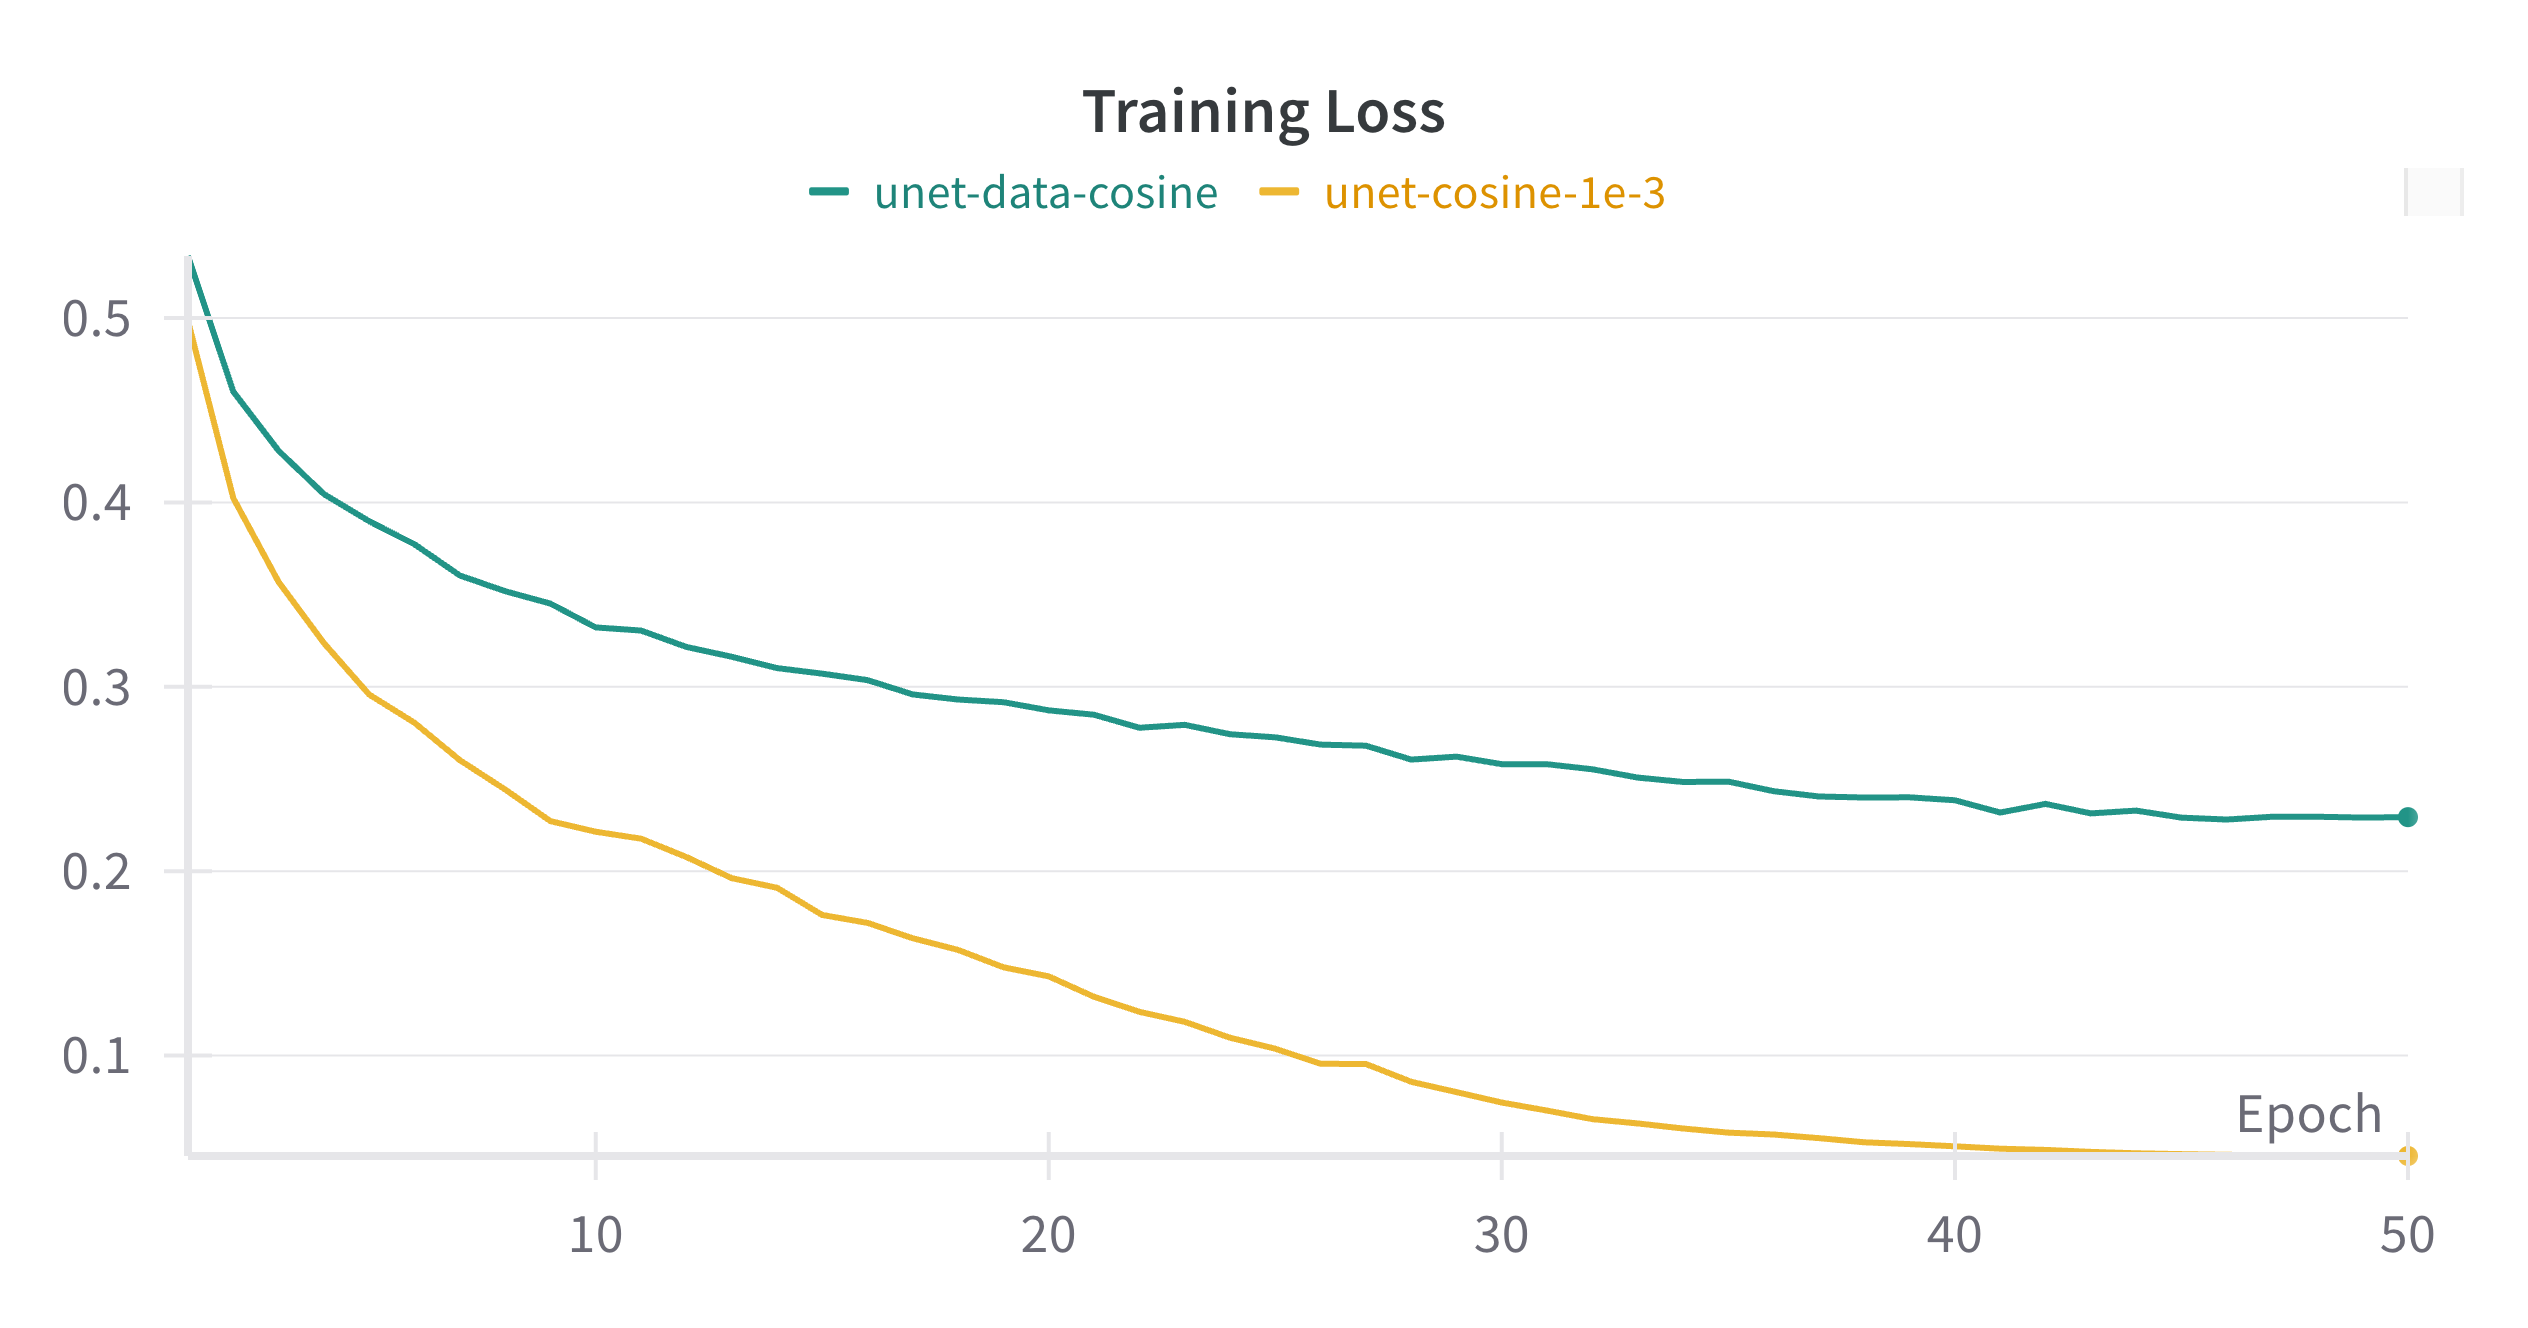
\includegraphics[width=0.95\linewidth]{figs/aug_unet_train_loss}
\caption{\textbf{The training loss over epochs.} \texttt{unet-data-cosine} is the model with data argumentation, while \texttt{unet-cosine-1e-3} is without data argumentation.}
\label{fig:augunettrainloss}
\end{figure}
\begin{figure}[H]
\centering
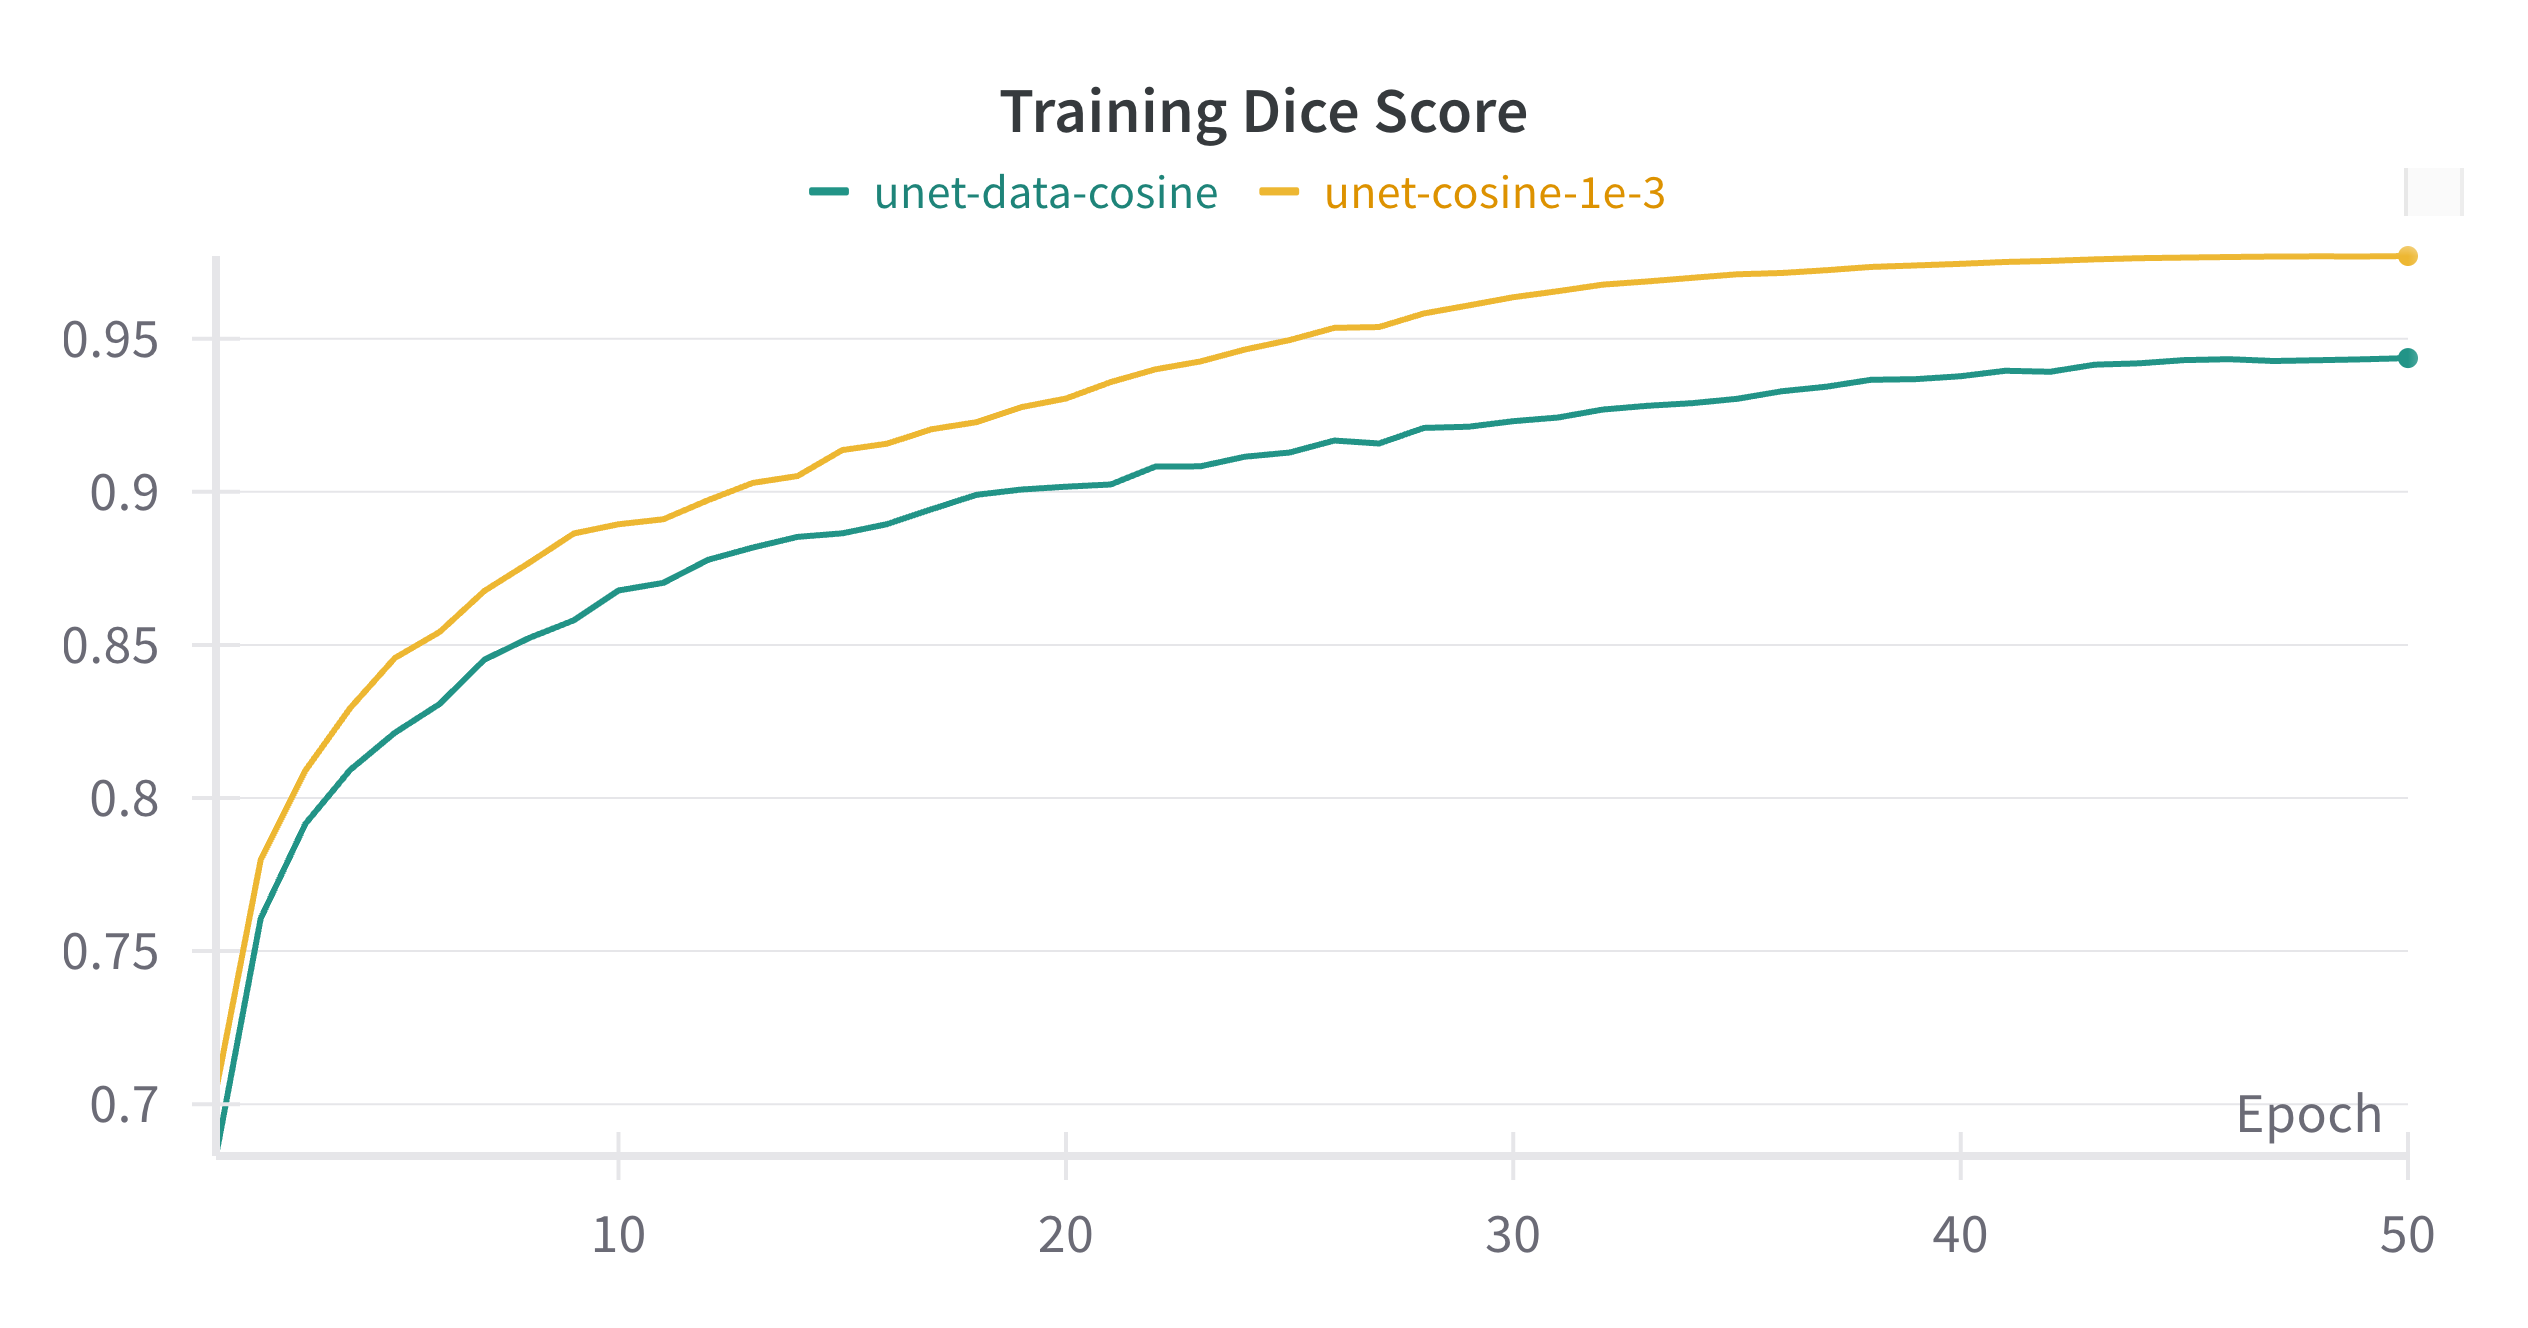
\includegraphics[width=0.95\linewidth]{figs/aug_unet_train_dice}
\caption{\textbf{The training Dice score over epochs.} \texttt{unet-data-cosine} is the model with data argumentation, while \texttt{unet-cosine-1e-3} is without data argumentation. The model without data argumentation achieves higher training Dice scores but performs worse on validation data.}
\label{fig:augunettraindice}
\end{figure}
\begin{figure}[H]
\centering
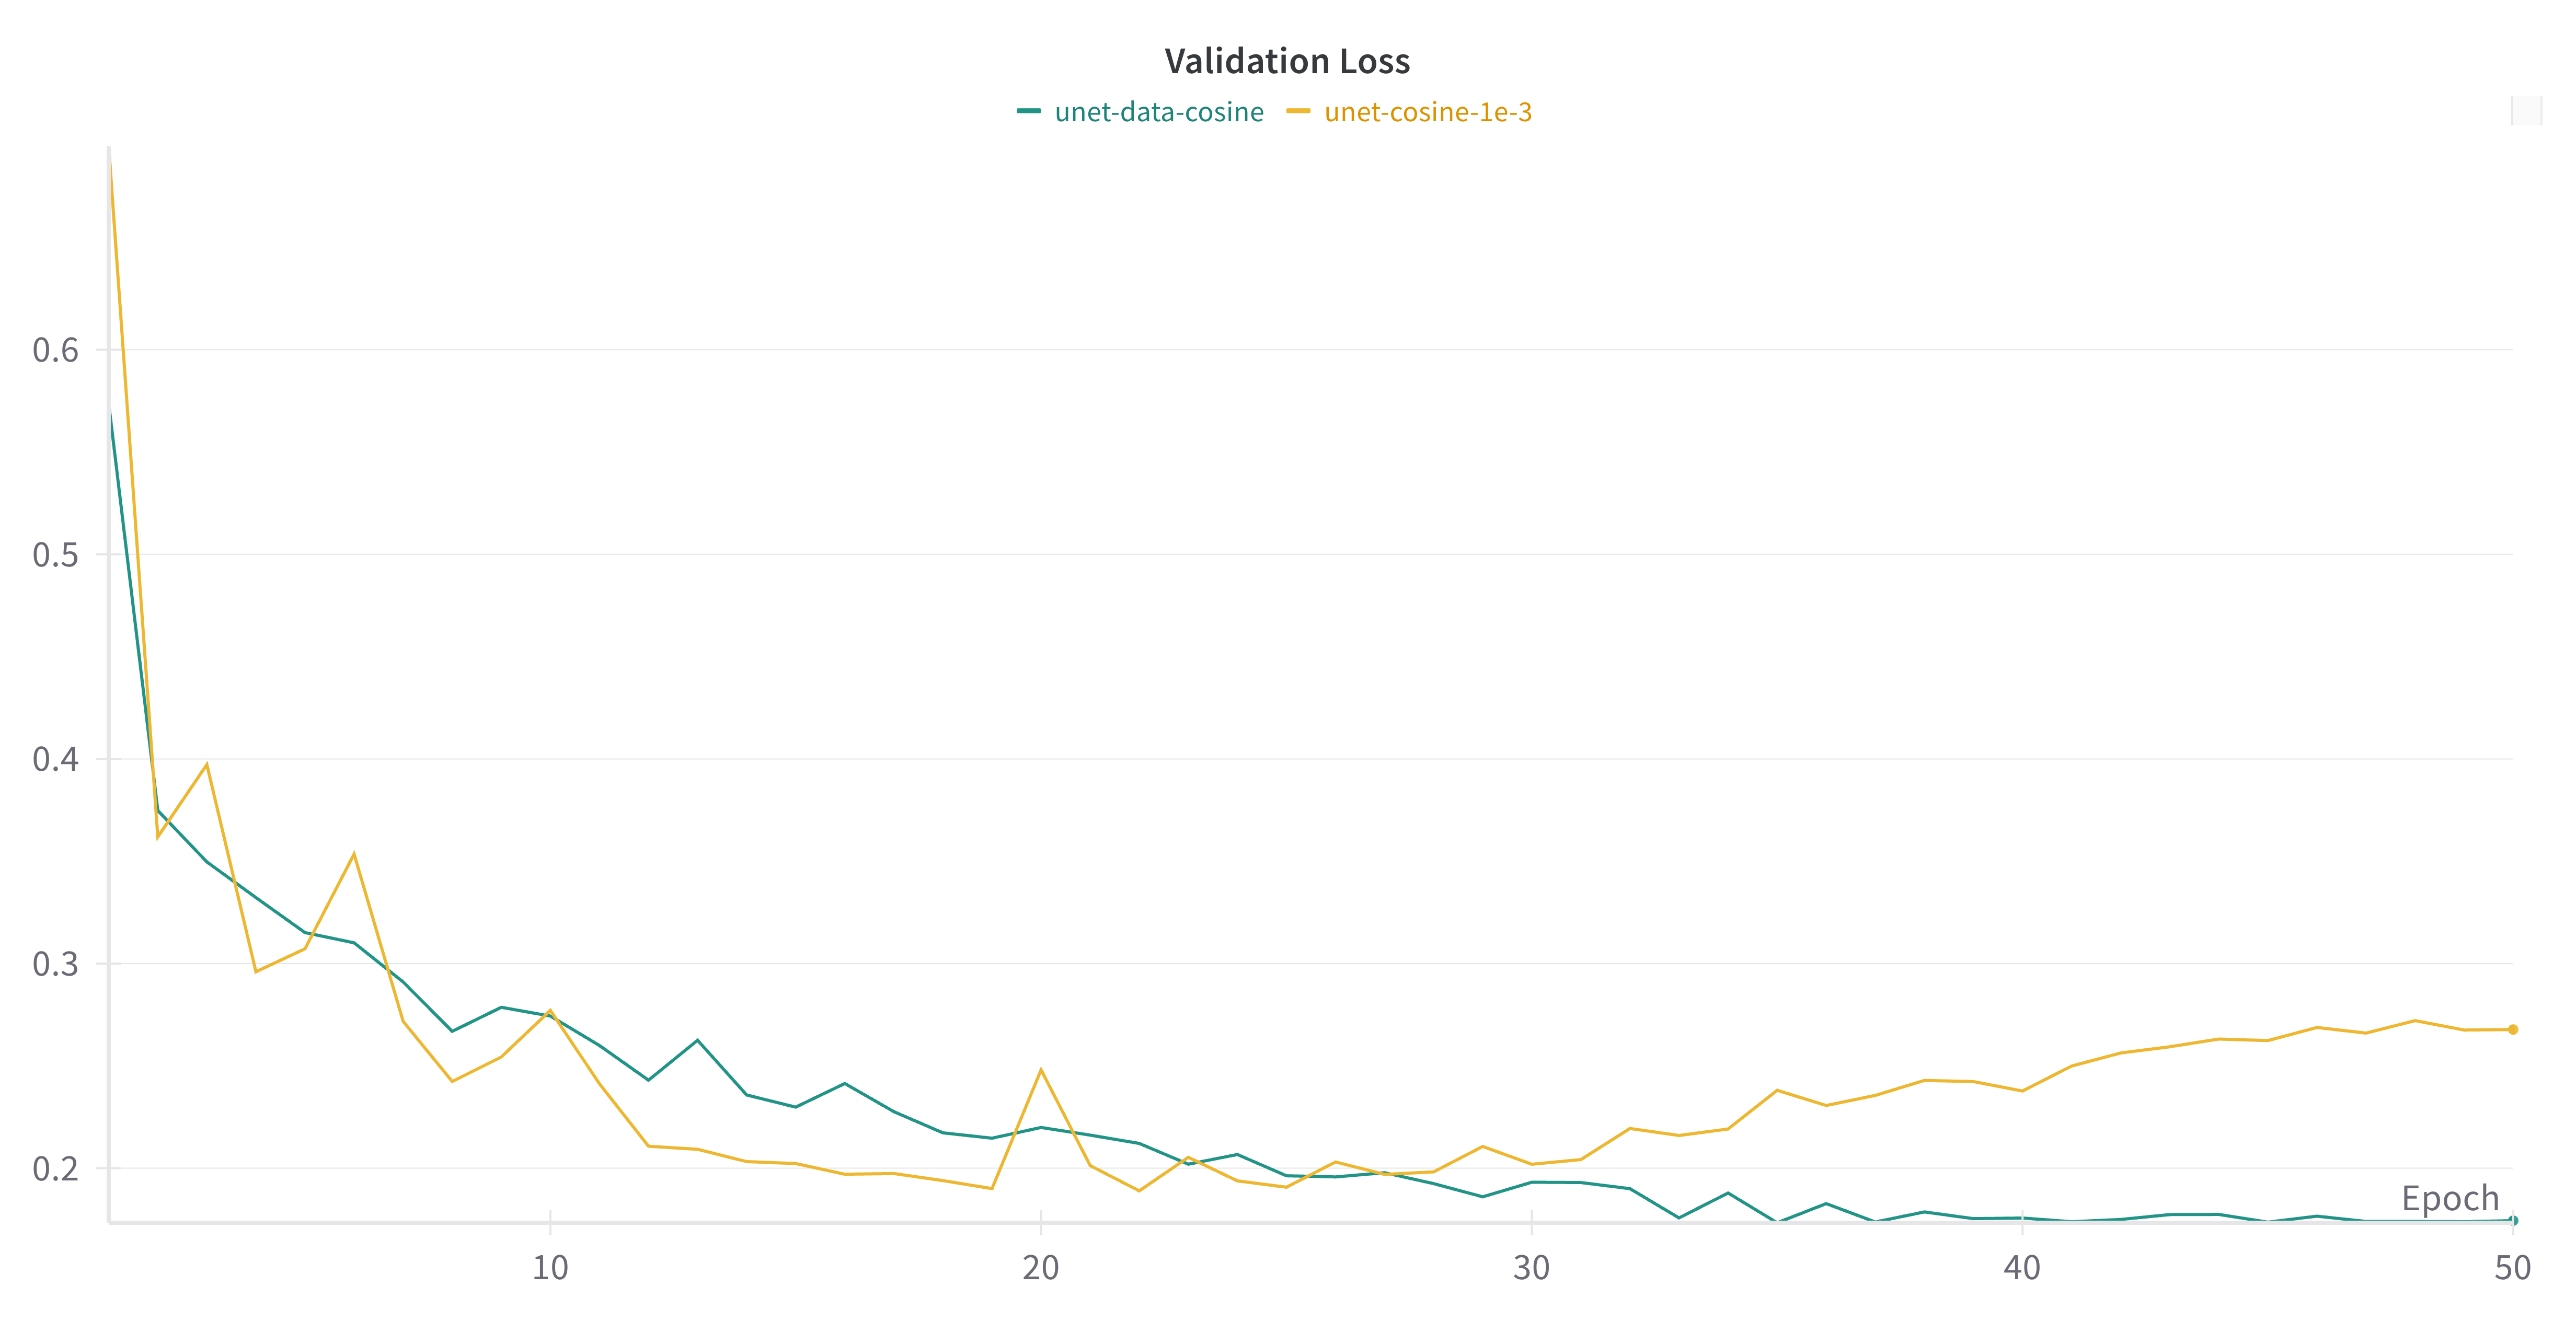
\includegraphics[width=0.95\linewidth]{figs/aug_unet_val_loss}
\caption{\textbf{The validation loss over epochs.} \texttt{unet-data-cosine} is the model with data argumentation, while \texttt{unet-cosine-1e-3} is without data argumentation. The validation loss for the model without data argumentation increases after epoch 25, indicating overfitting.}
\label{fig:augunetvalloss}
\end{figure}
\begin{figure}[H]
\centering
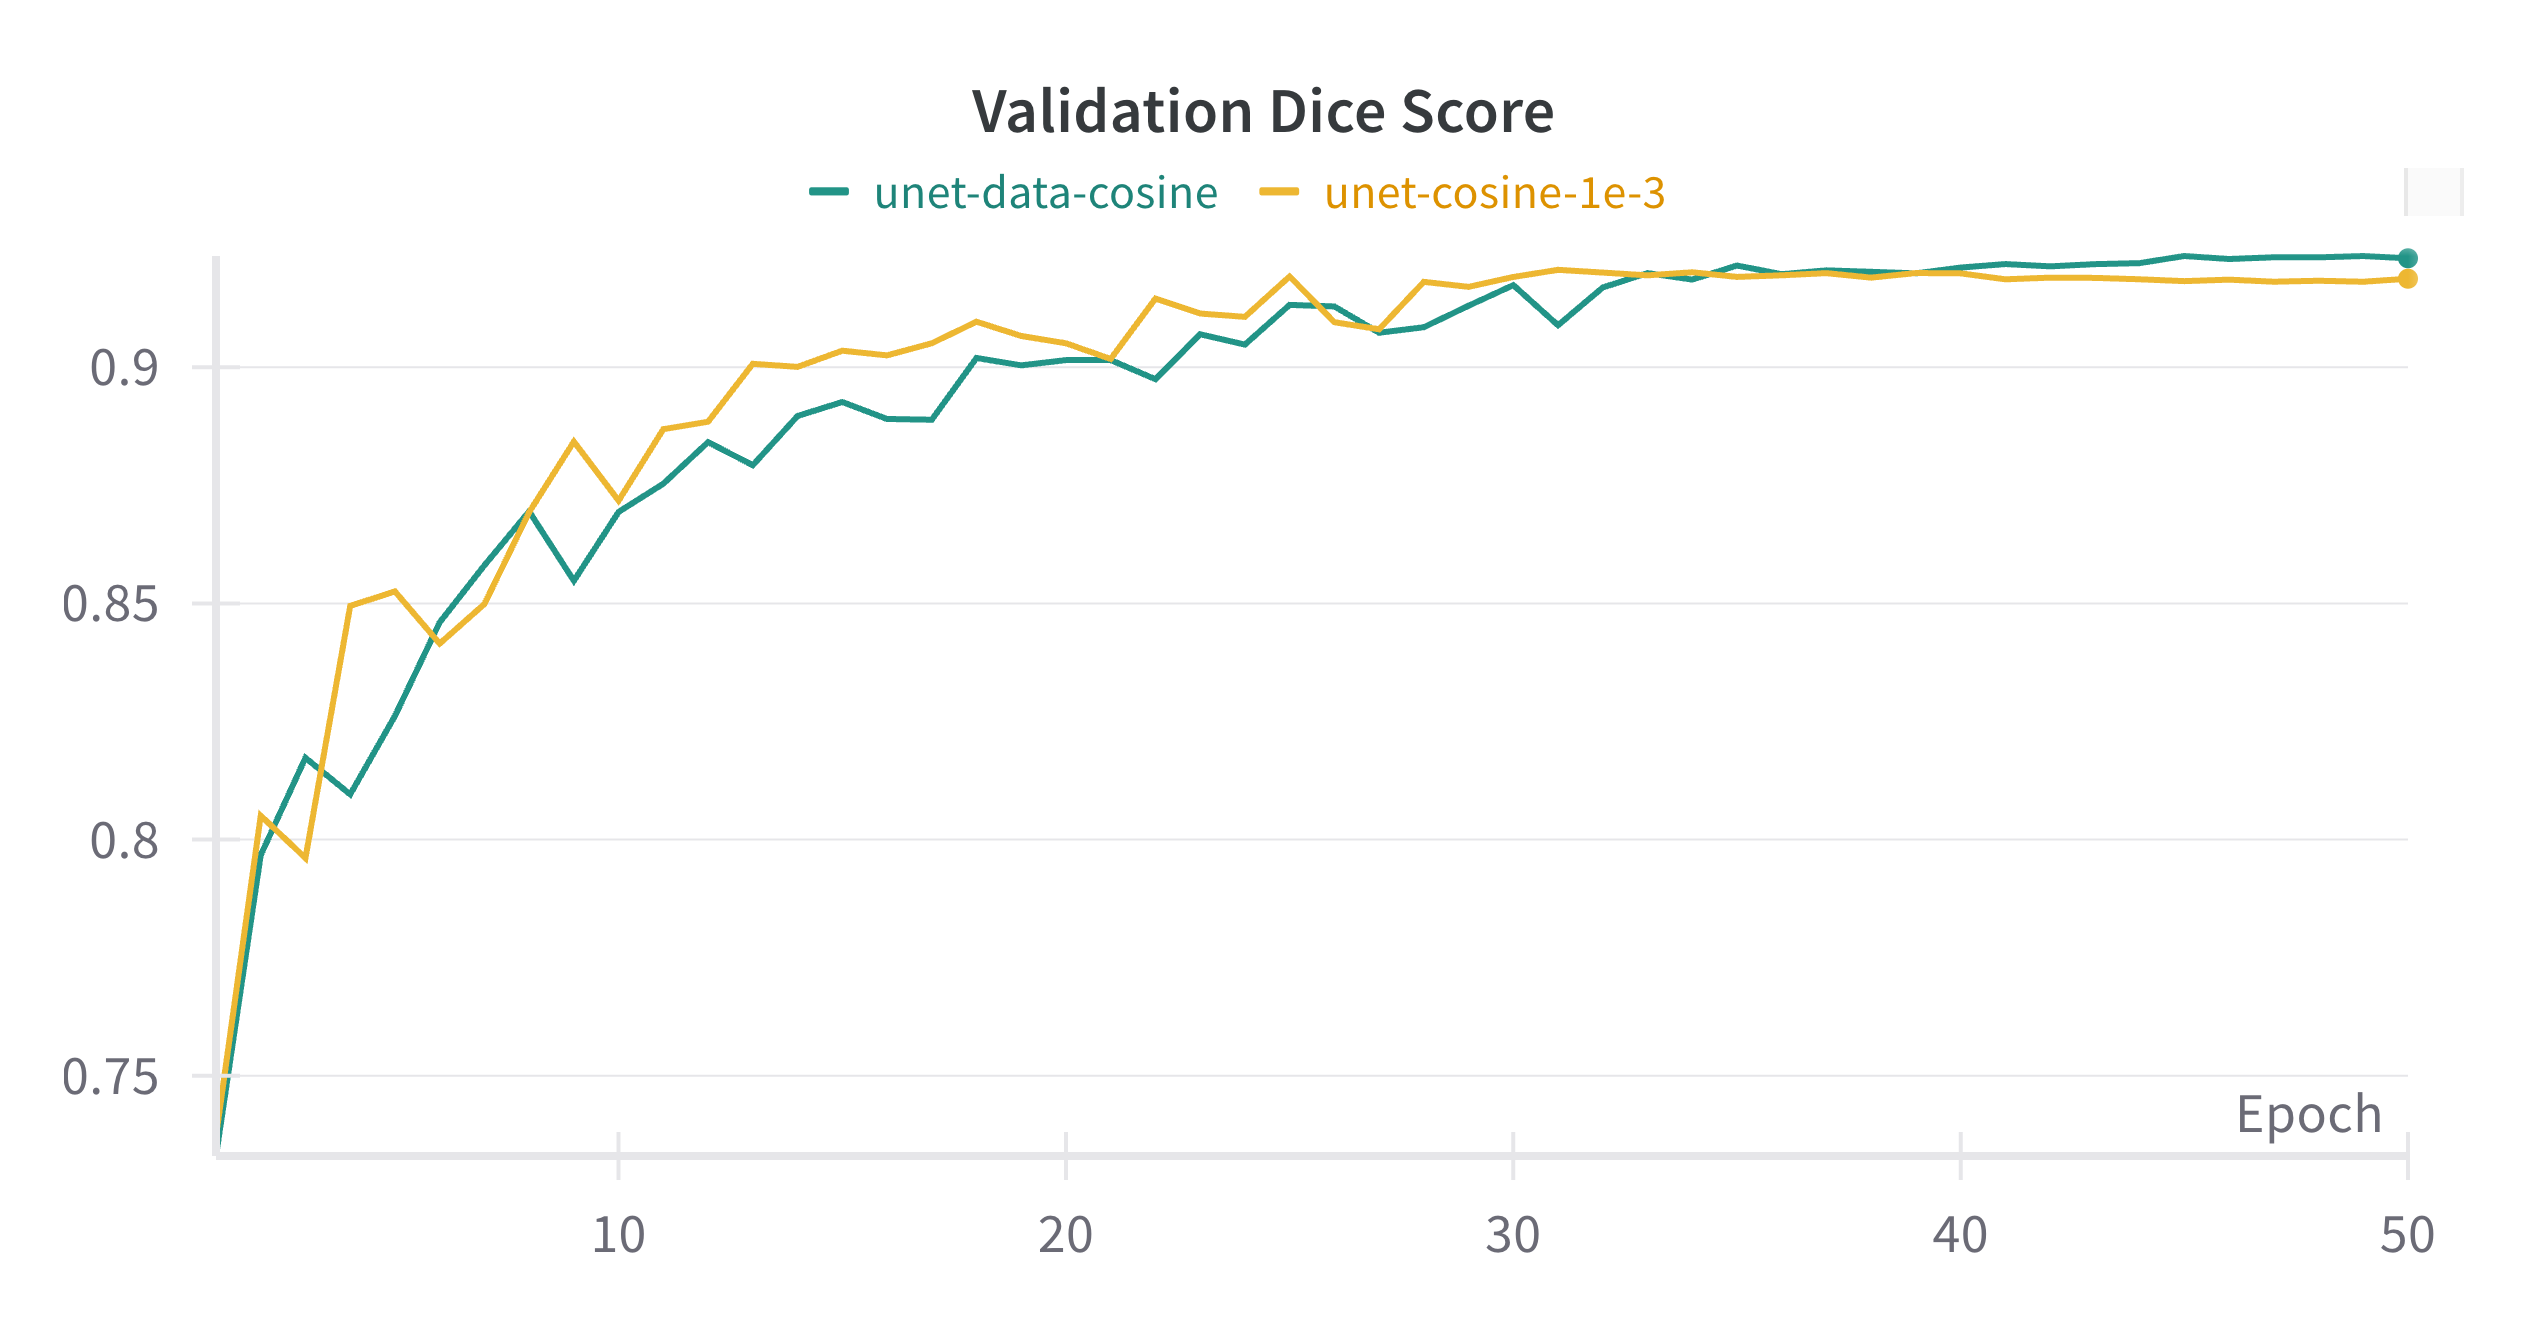
\includegraphics[width=0.95\linewidth]{figs/aug_unet_val_dice}
\caption{\textbf{The validation Dice score over epochs.} \texttt{unet-data-cosine} is the model with data argumentation, while \texttt{unet-cosine-1e-3} is without data argumentation. Data argumentation helps maintain higher validation Dice scores throughout training, demonstrating better generalization.}
\label{fig:augunetvaldice}
\end{figure}


\paragraph{ResNet34\_U-Net.} We observe similar validation loss behavior on the ResNet34\_U-Net architecture. As shown in \autoref{fig:augresnettrainloss} and \autoref{fig:augresnettraindice}, the model without data augmentation achieves lower training loss and higher training Dice scores initially. However, examining the validation metrics reveals the same pattern of overfitting. In \autoref{fig:augresnetvalloss}, we can see that the validation loss for the non-augmented model begins to increase around epoch 20, while the augmented model maintains a steadier, lower validation loss throughout training. This translates to superior validation Dice scores for the augmented model, as displayed in \autoref{fig:augresnetvaldice}.

\begin{figure}[H]
\centering
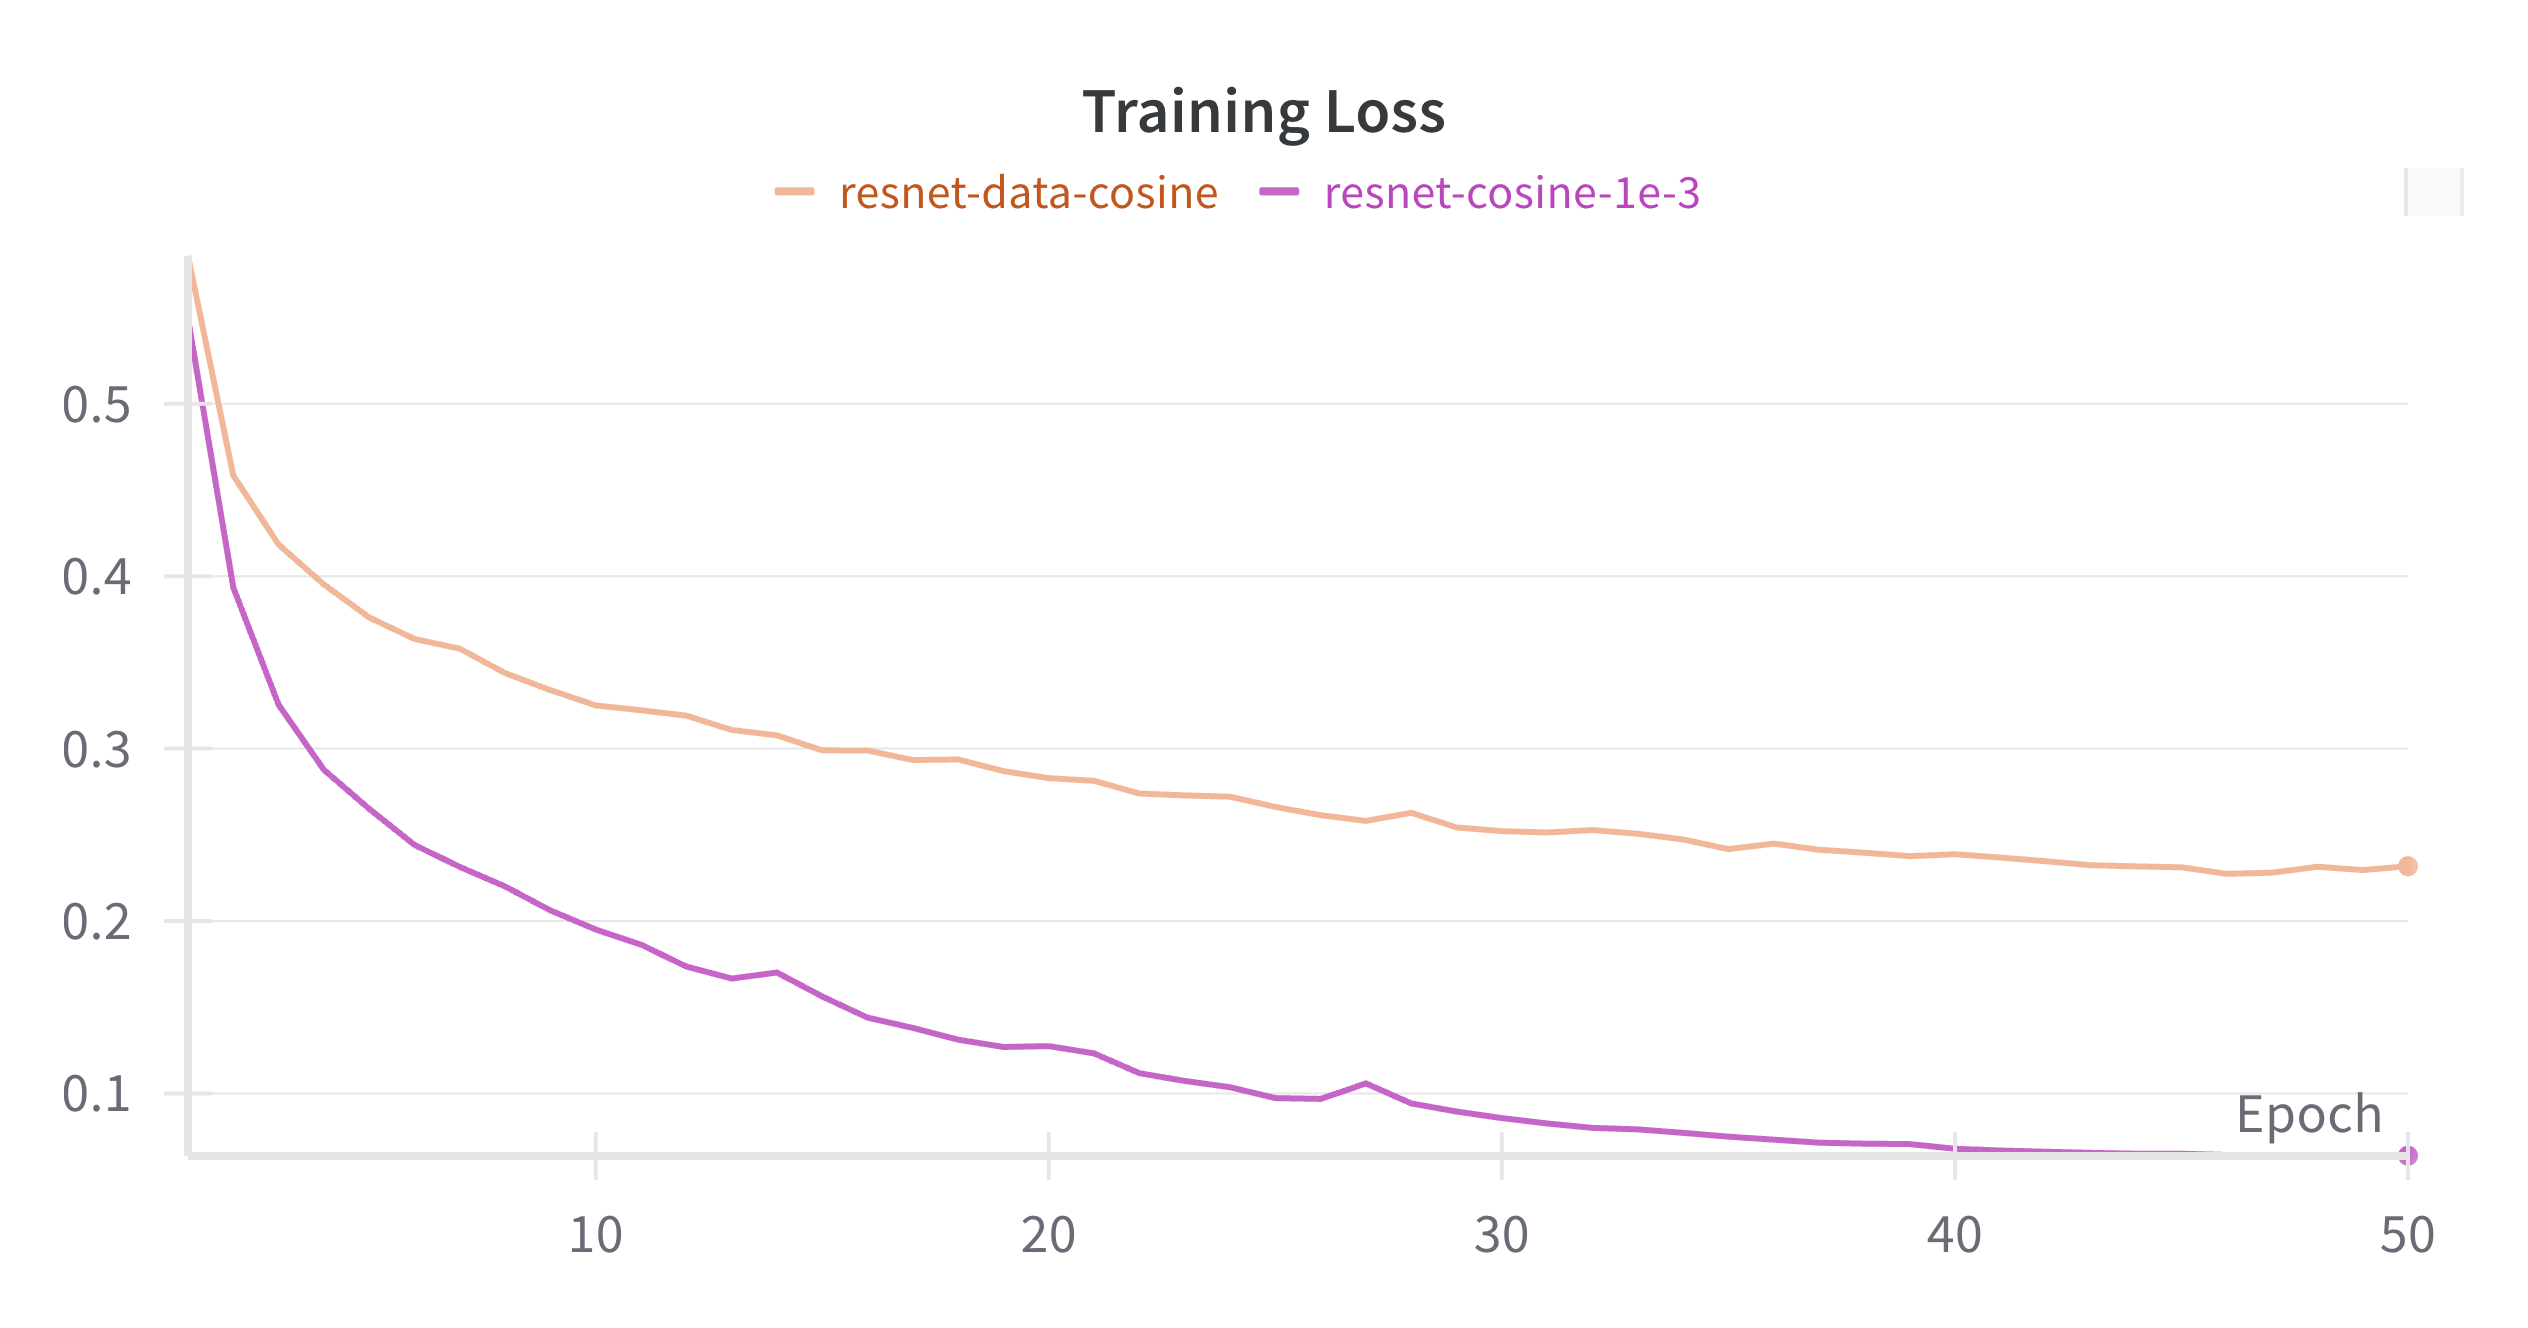
\includegraphics[width=0.95\linewidth]{figs/aug_resnet_train_loss}
\caption{\textbf{The training loss over epochs for ResNet34\_U-Net.} \texttt{resnet-data-cosine} is the model with data augmentation, while \texttt{resnet-cosine-1e-3} is without data augmentation.}
\label{fig:augresnettrainloss}
\end{figure}
\begin{figure}[H]
\centering
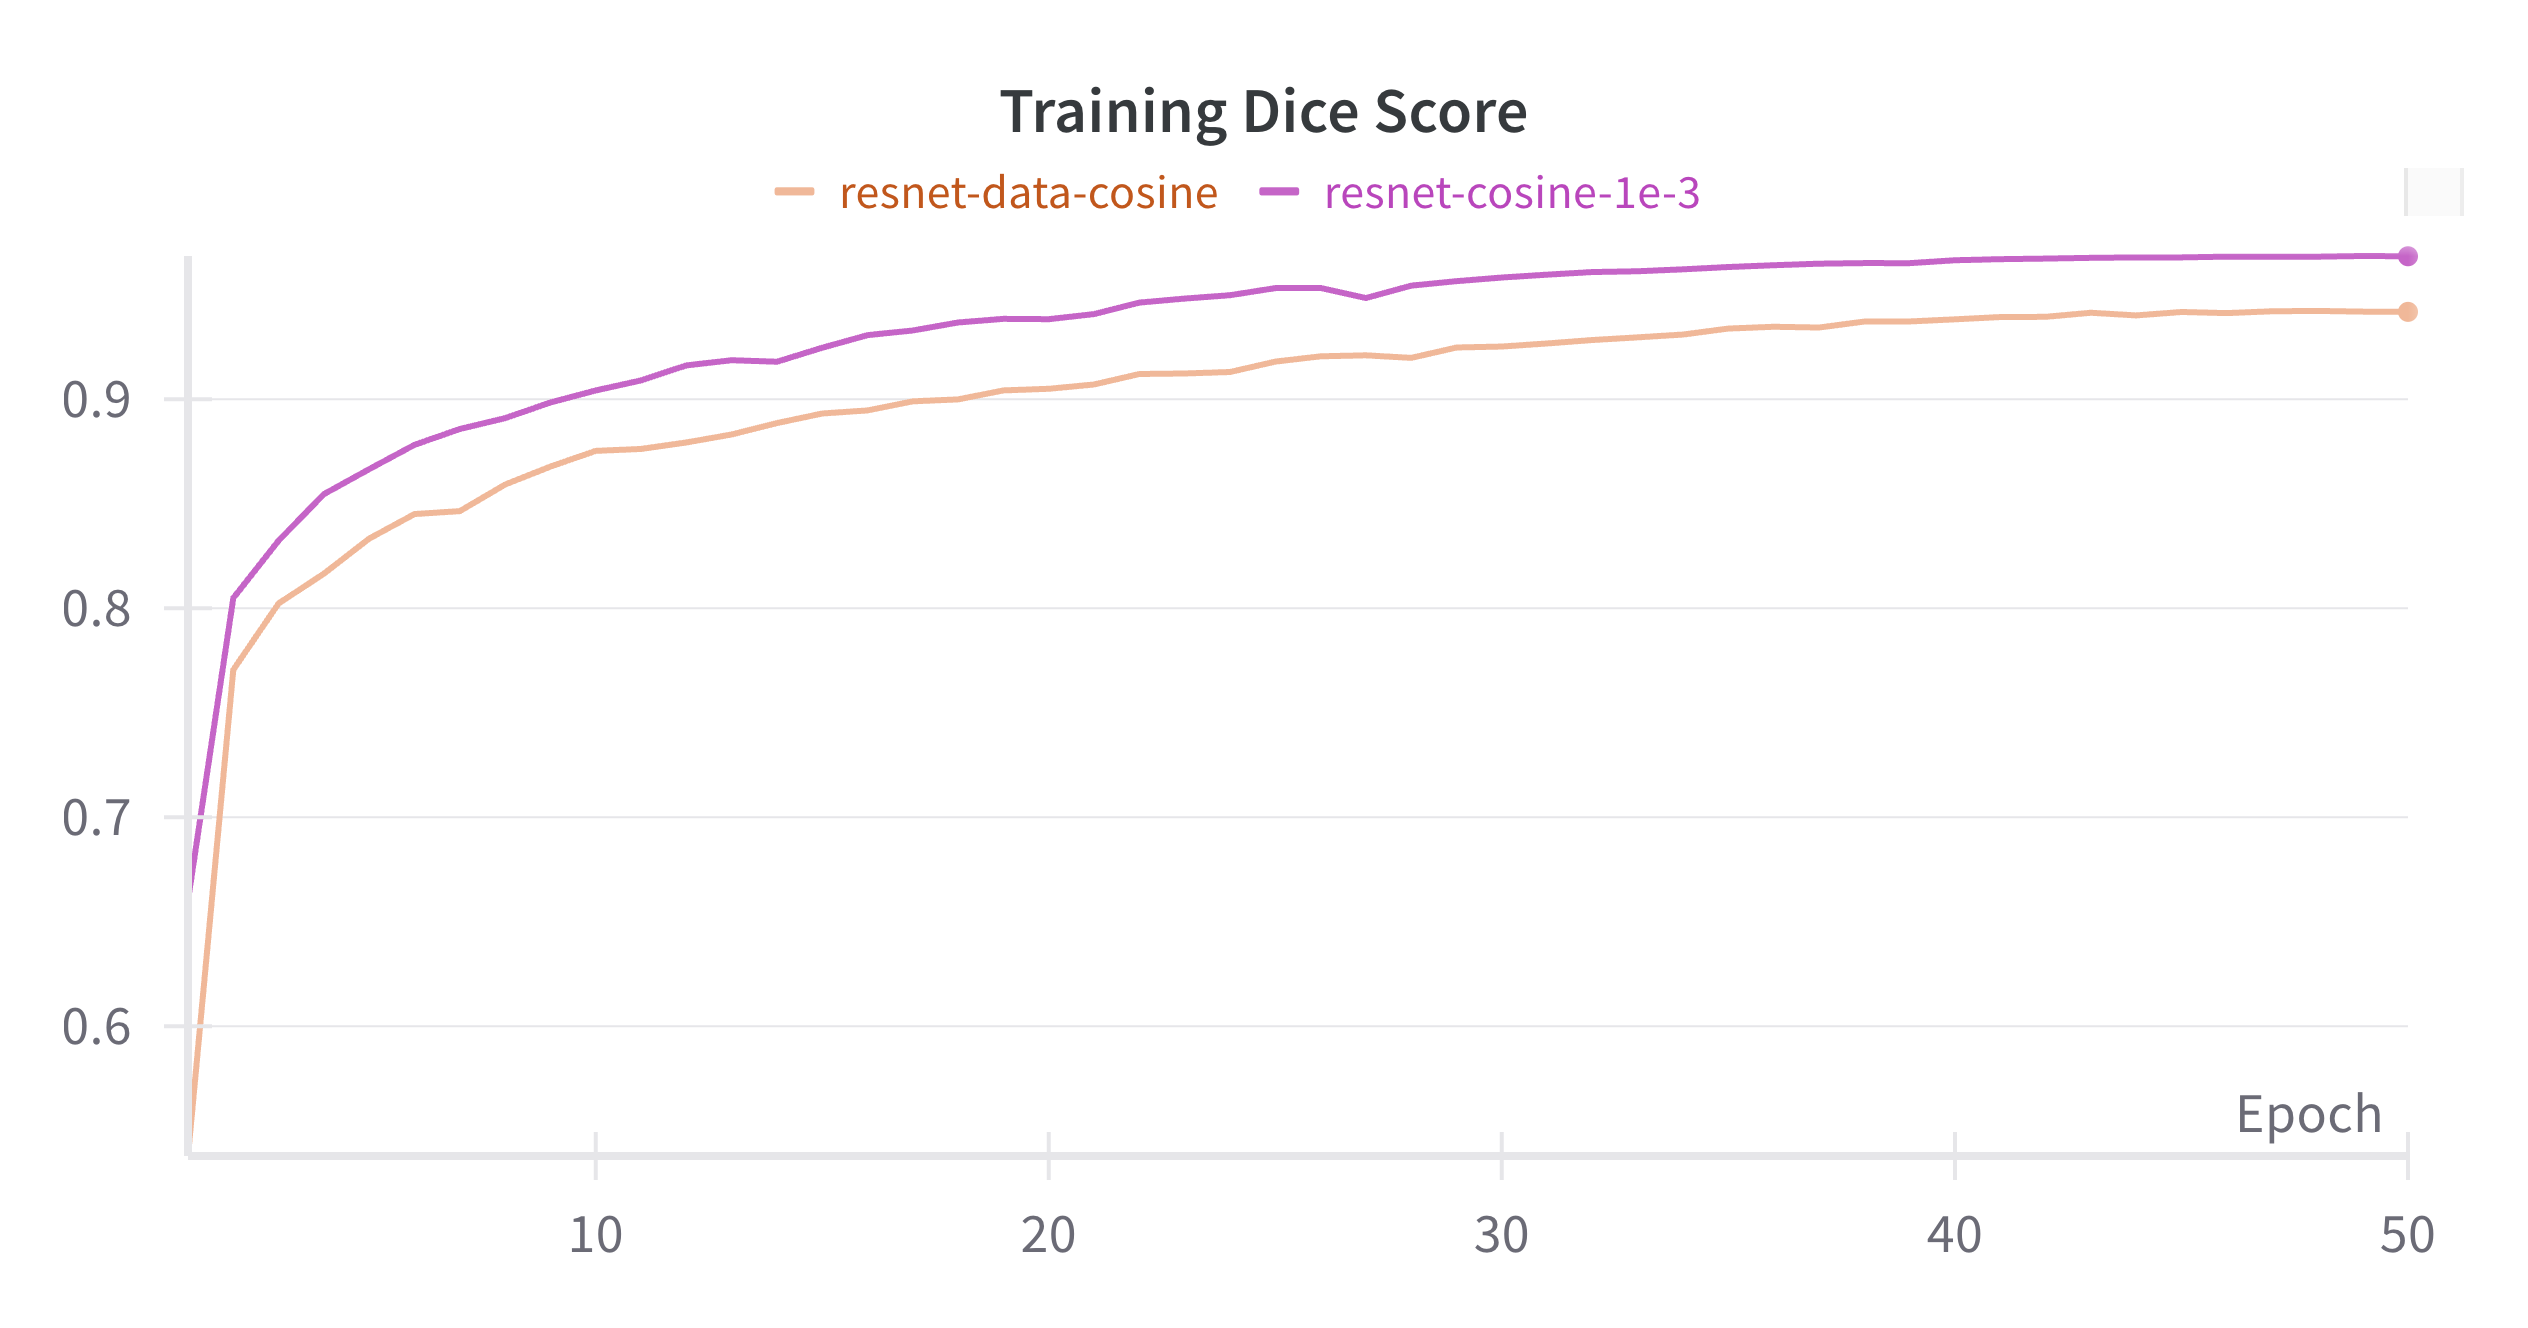
\includegraphics[width=0.95\linewidth]{figs/aug_resnet_train_dice}
\caption{\textbf{The training Dice score over epochs for ResNet34\_U-Net.} \texttt{resnet-data-cosine} is the model with data augmentation, while \texttt{resnet-cosine-1e-3} is without data augmentation. The non-augmented model shows higher training Dice scores but fails to generalize as well to validation data.}
\label{fig:augresnettraindice}
\end{figure}
\begin{figure}[H]
\centering
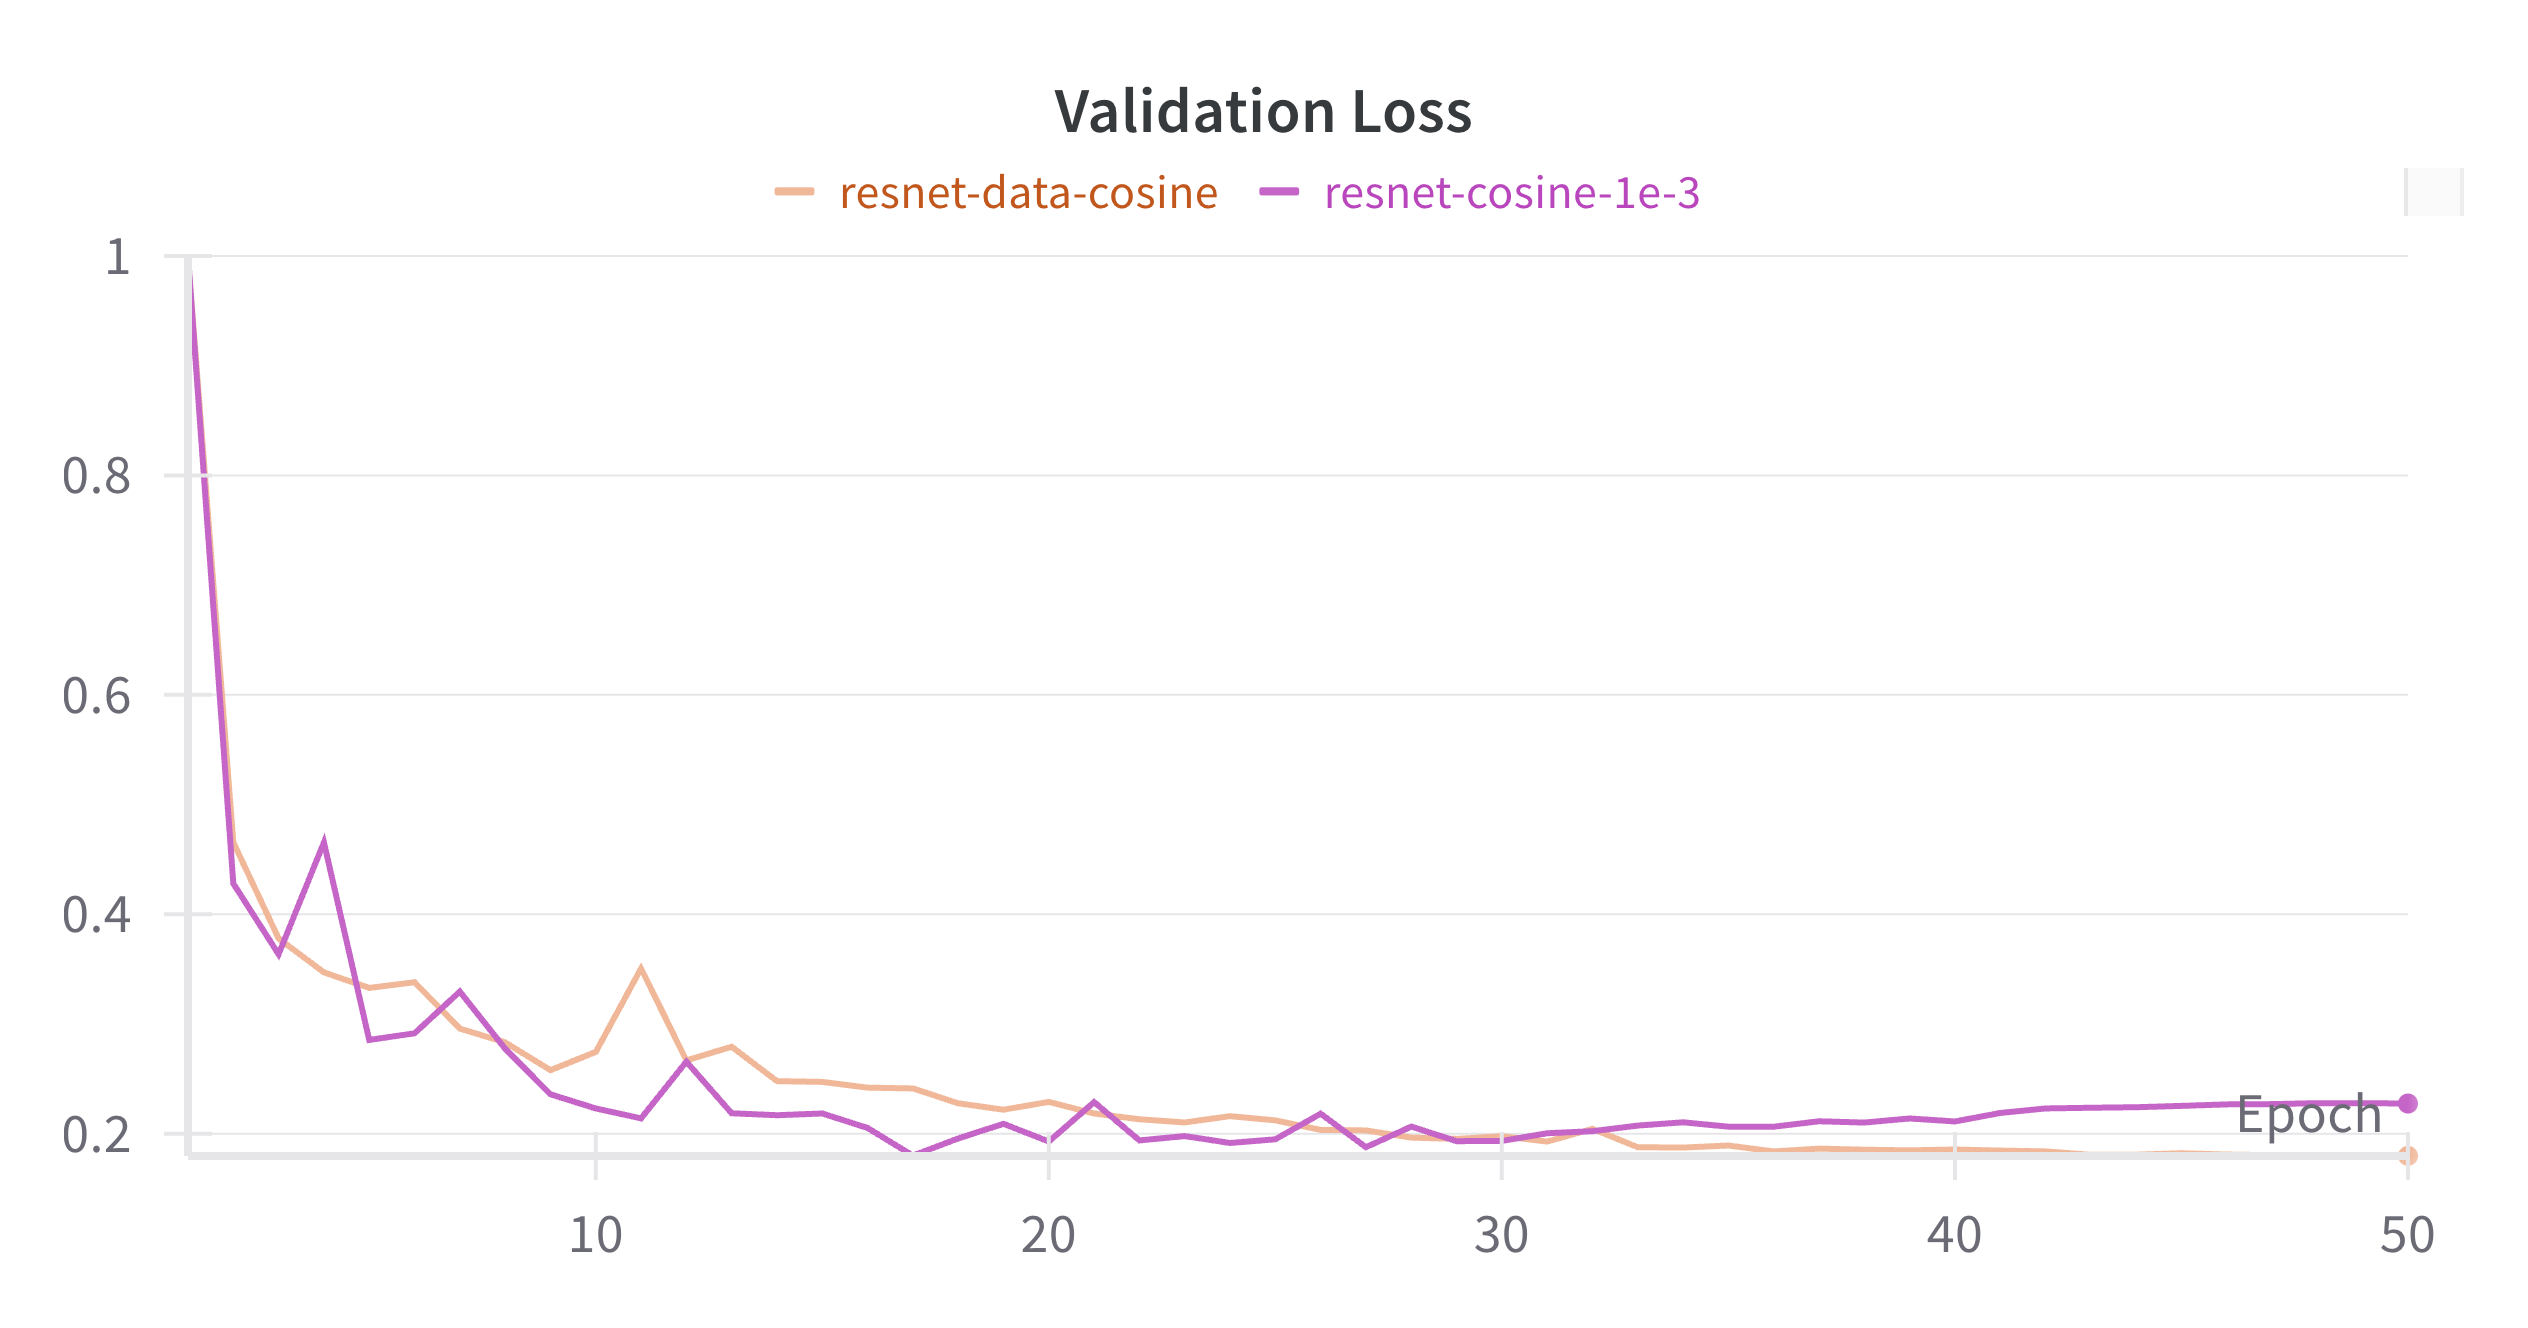
\includegraphics[width=0.95\linewidth]{figs/aug_resnet_val_loss}
\caption{\textbf{The validation loss over epochs for ResNet34\_U-Net.} \texttt{resnet-data-cosine} is the model with data augmentation, while \texttt{resnet-cosine-1e-3} is without data augmentation. The validation loss for the non-augmented model increases after epoch 20, indicating overfitting.}
\label{fig:augresnetvalloss}
\end{figure}
\begin{figure}[H]
\centering
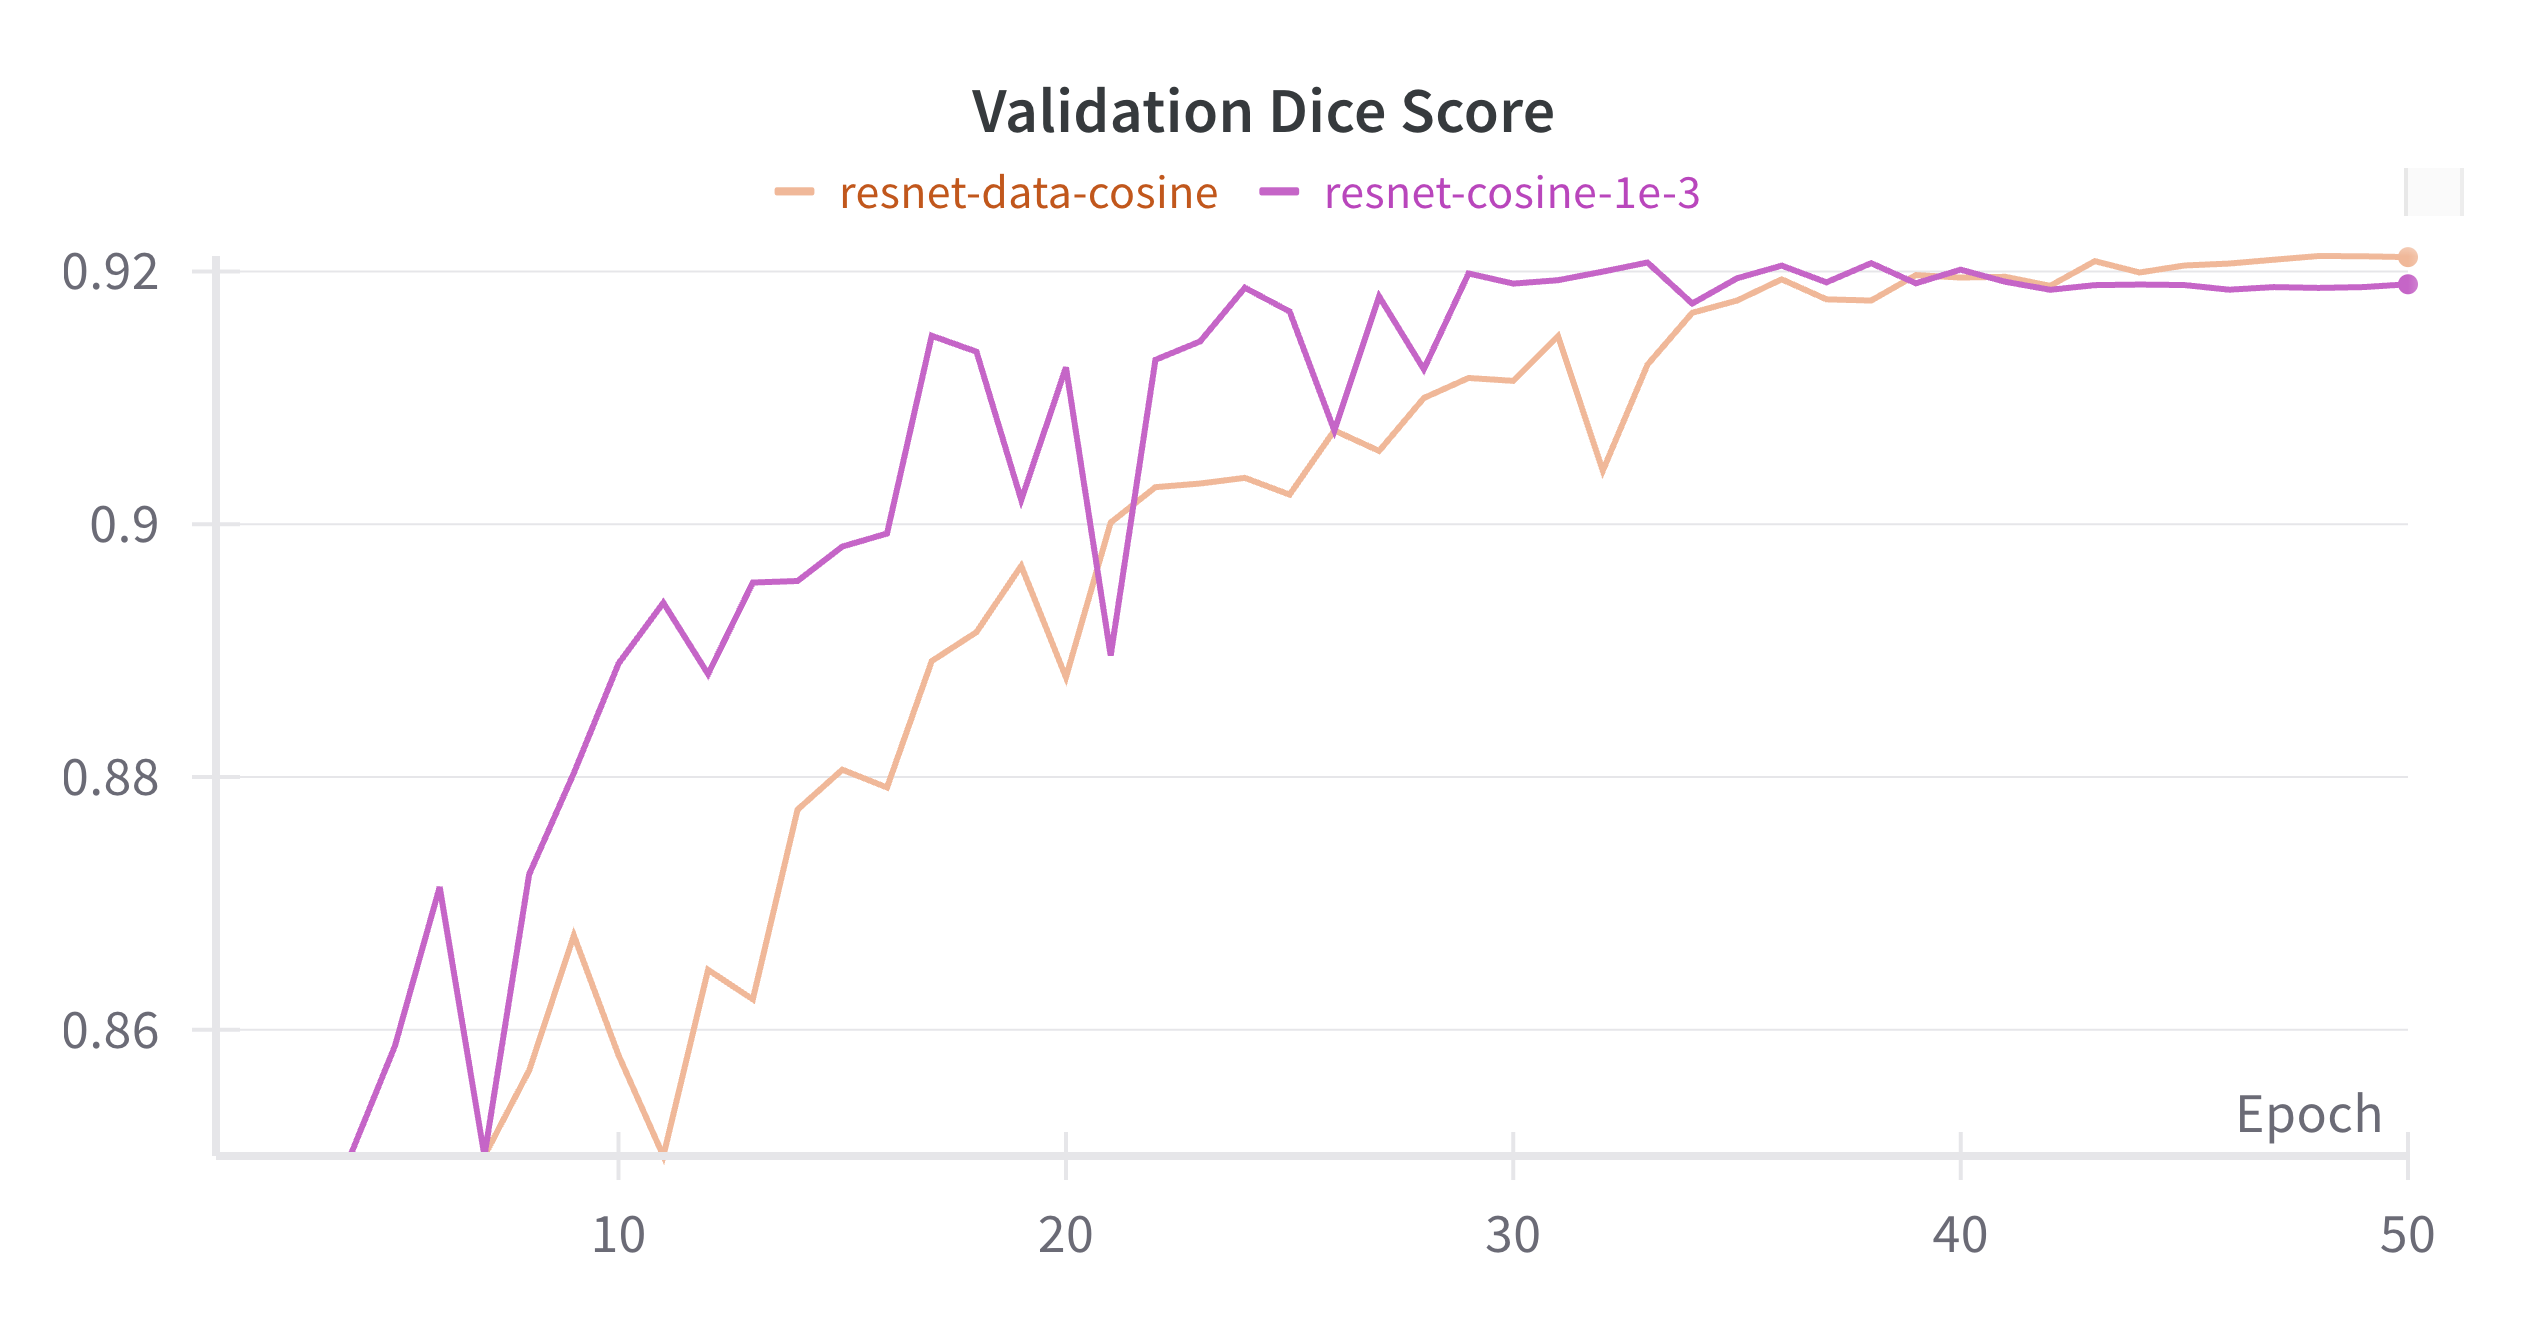
\includegraphics[width=0.95\linewidth]{figs/aug_resnet_val_dice}
\caption{\textbf{The validation Dice score over epochs for ResNet34\_U-Net.} \texttt{resnet-data-cosine} is the model with data augmentation, while \texttt{resnet-cosine-1e-3} is without data augmentation. The augmented model demonstrates more stable and higher validation performance throughout training.}
\label{fig:augresnetvaldice}
\end{figure}

Based on these consistent findings across both architectures, we conclude that data augmentation is essential for mitigating overfitting and improving generalization in semantic segmentation tasks with the Oxford-IIIT Pet Dataset. The augmentation techniques, including random horizontal and vertical flips and color jittering, effectively increase the diversity of the training data without requiring additional labeled samples. This approach leads to more robust models that perform better on unseen data. Therefore, we will apply data augmentation in all successive experiments to ensure optimal model performance and generalization capability.



\subsection{Learning rate scheduling}
In this experiment, I evaluated both models using two different learning rate schedulers: CosineAnnealingLR and OneCycleLR. The CosineAnnealingLR scheduler follows a cosine wave function to gradually decrease the learning rate from its initial value to near-zero over the training period. In contrast, the OneCycleLR scheduler implements a three-phase approach: it begins with a low initial learning rate, gradually increases it during the first 10\% of training epochs until reaching the maximum specified value, and then decreases it following a cosine curve back to a minimal value by the end of training. This comparison allows us to assess how different learning rate trajectories affect model convergence and final performance.

\paragraph{U-Net.} For the U-Net architecture, we observe distinct differences in training dynamics between the two schedulers. As shown in \autoref{fig:lrunetlr}, the learning rate trajectories differ significantly, with OneCycleLR featuring an initial warm-up phase followed by a steeper decline. This learning rate pattern appears to benefit the U-Net model, as evidenced by the training loss in \autoref{fig:lrunettrainloss} and training Dice score in \autoref{fig:lrunettraindice}. The OneCycleLR scheduler achieves lower training loss and higher training Dice scores, particularly in the later stages of training.

More importantly, the validation metrics demonstrate the superiority of the OneCycleLR approach. In \autoref{fig:lrunetvalloss}, we can see that the validation loss for the OneCycleLR-trained model is consistently lower after the initial epochs, suggesting better generalization. This translates to higher validation Dice scores as illustrated in \autoref{fig:lrunetvaldice}, with the OneCycleLR model maintaining a clear advantage throughout most of the training process.

\begin{figure}[H]
\centering
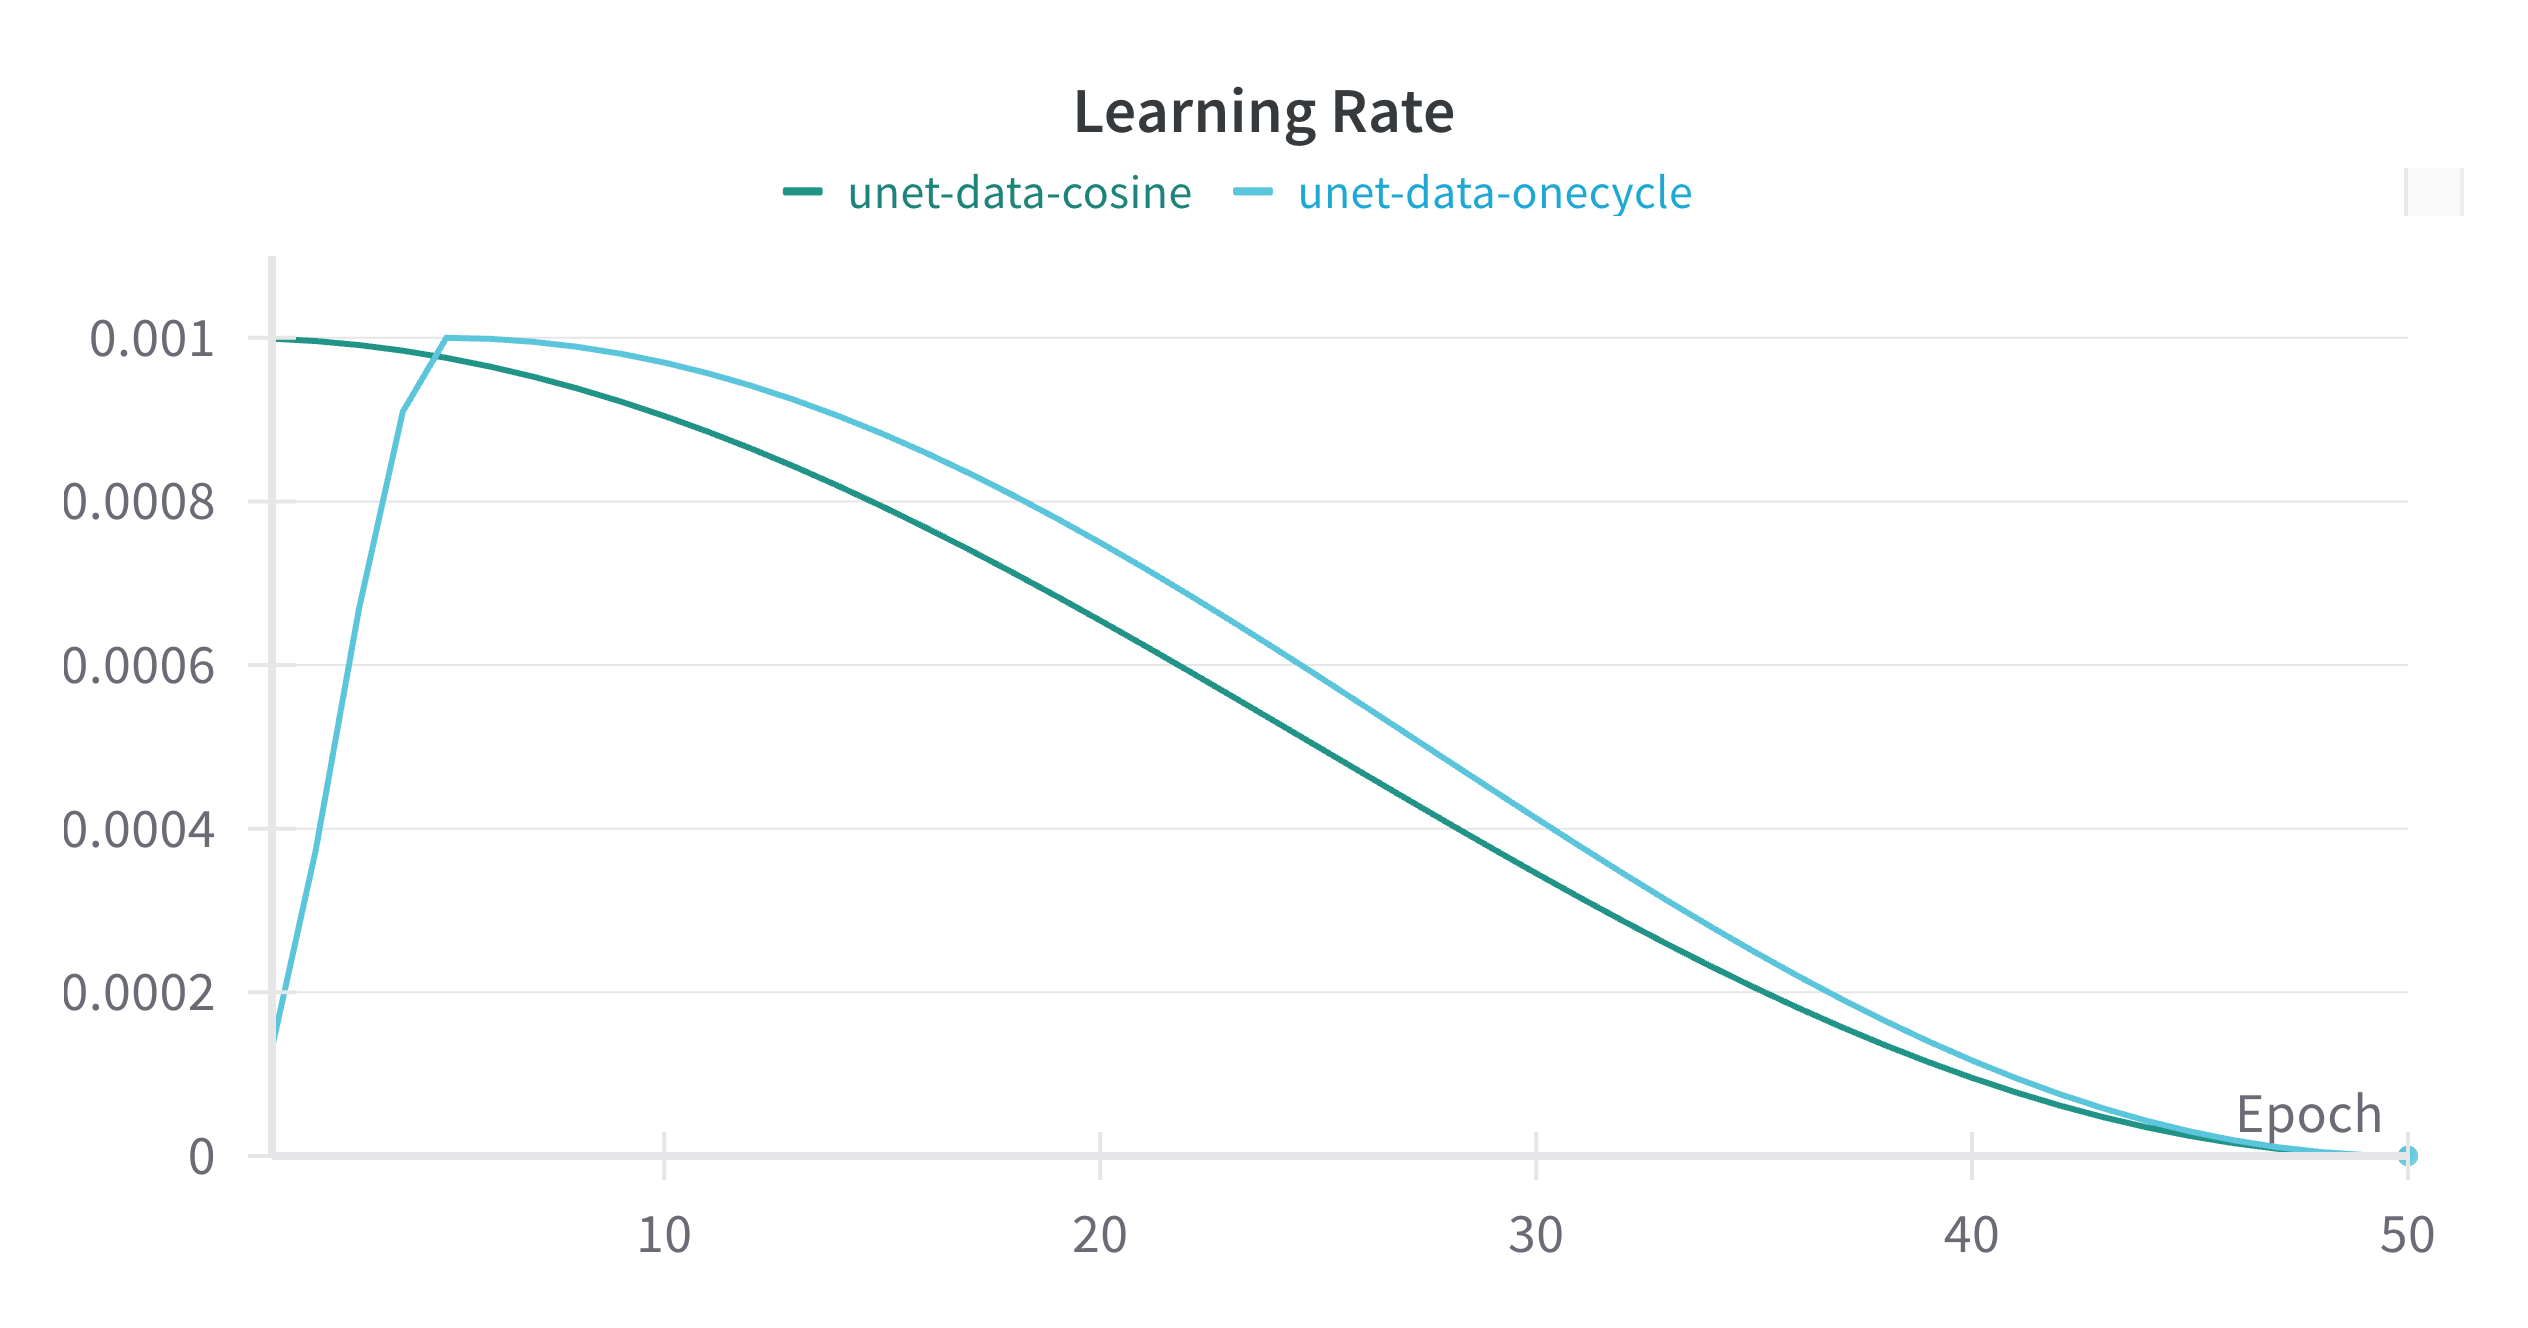
\includegraphics[width=0.95\linewidth]{figs/lr_unet_lr}
\caption{\textbf{Learning rate over epochs for U-Net models.} \texttt{unet-data-cosine} uses the CosineAnnealingLR scheduler, while \texttt{unet-data-onecycle} uses the OneCycleLR scheduler. Note the distinctive warm-up phase in the OneCycleLR approach.}
\label{fig:lrunetlr}
\end{figure}
\begin{figure}[H]
\centering
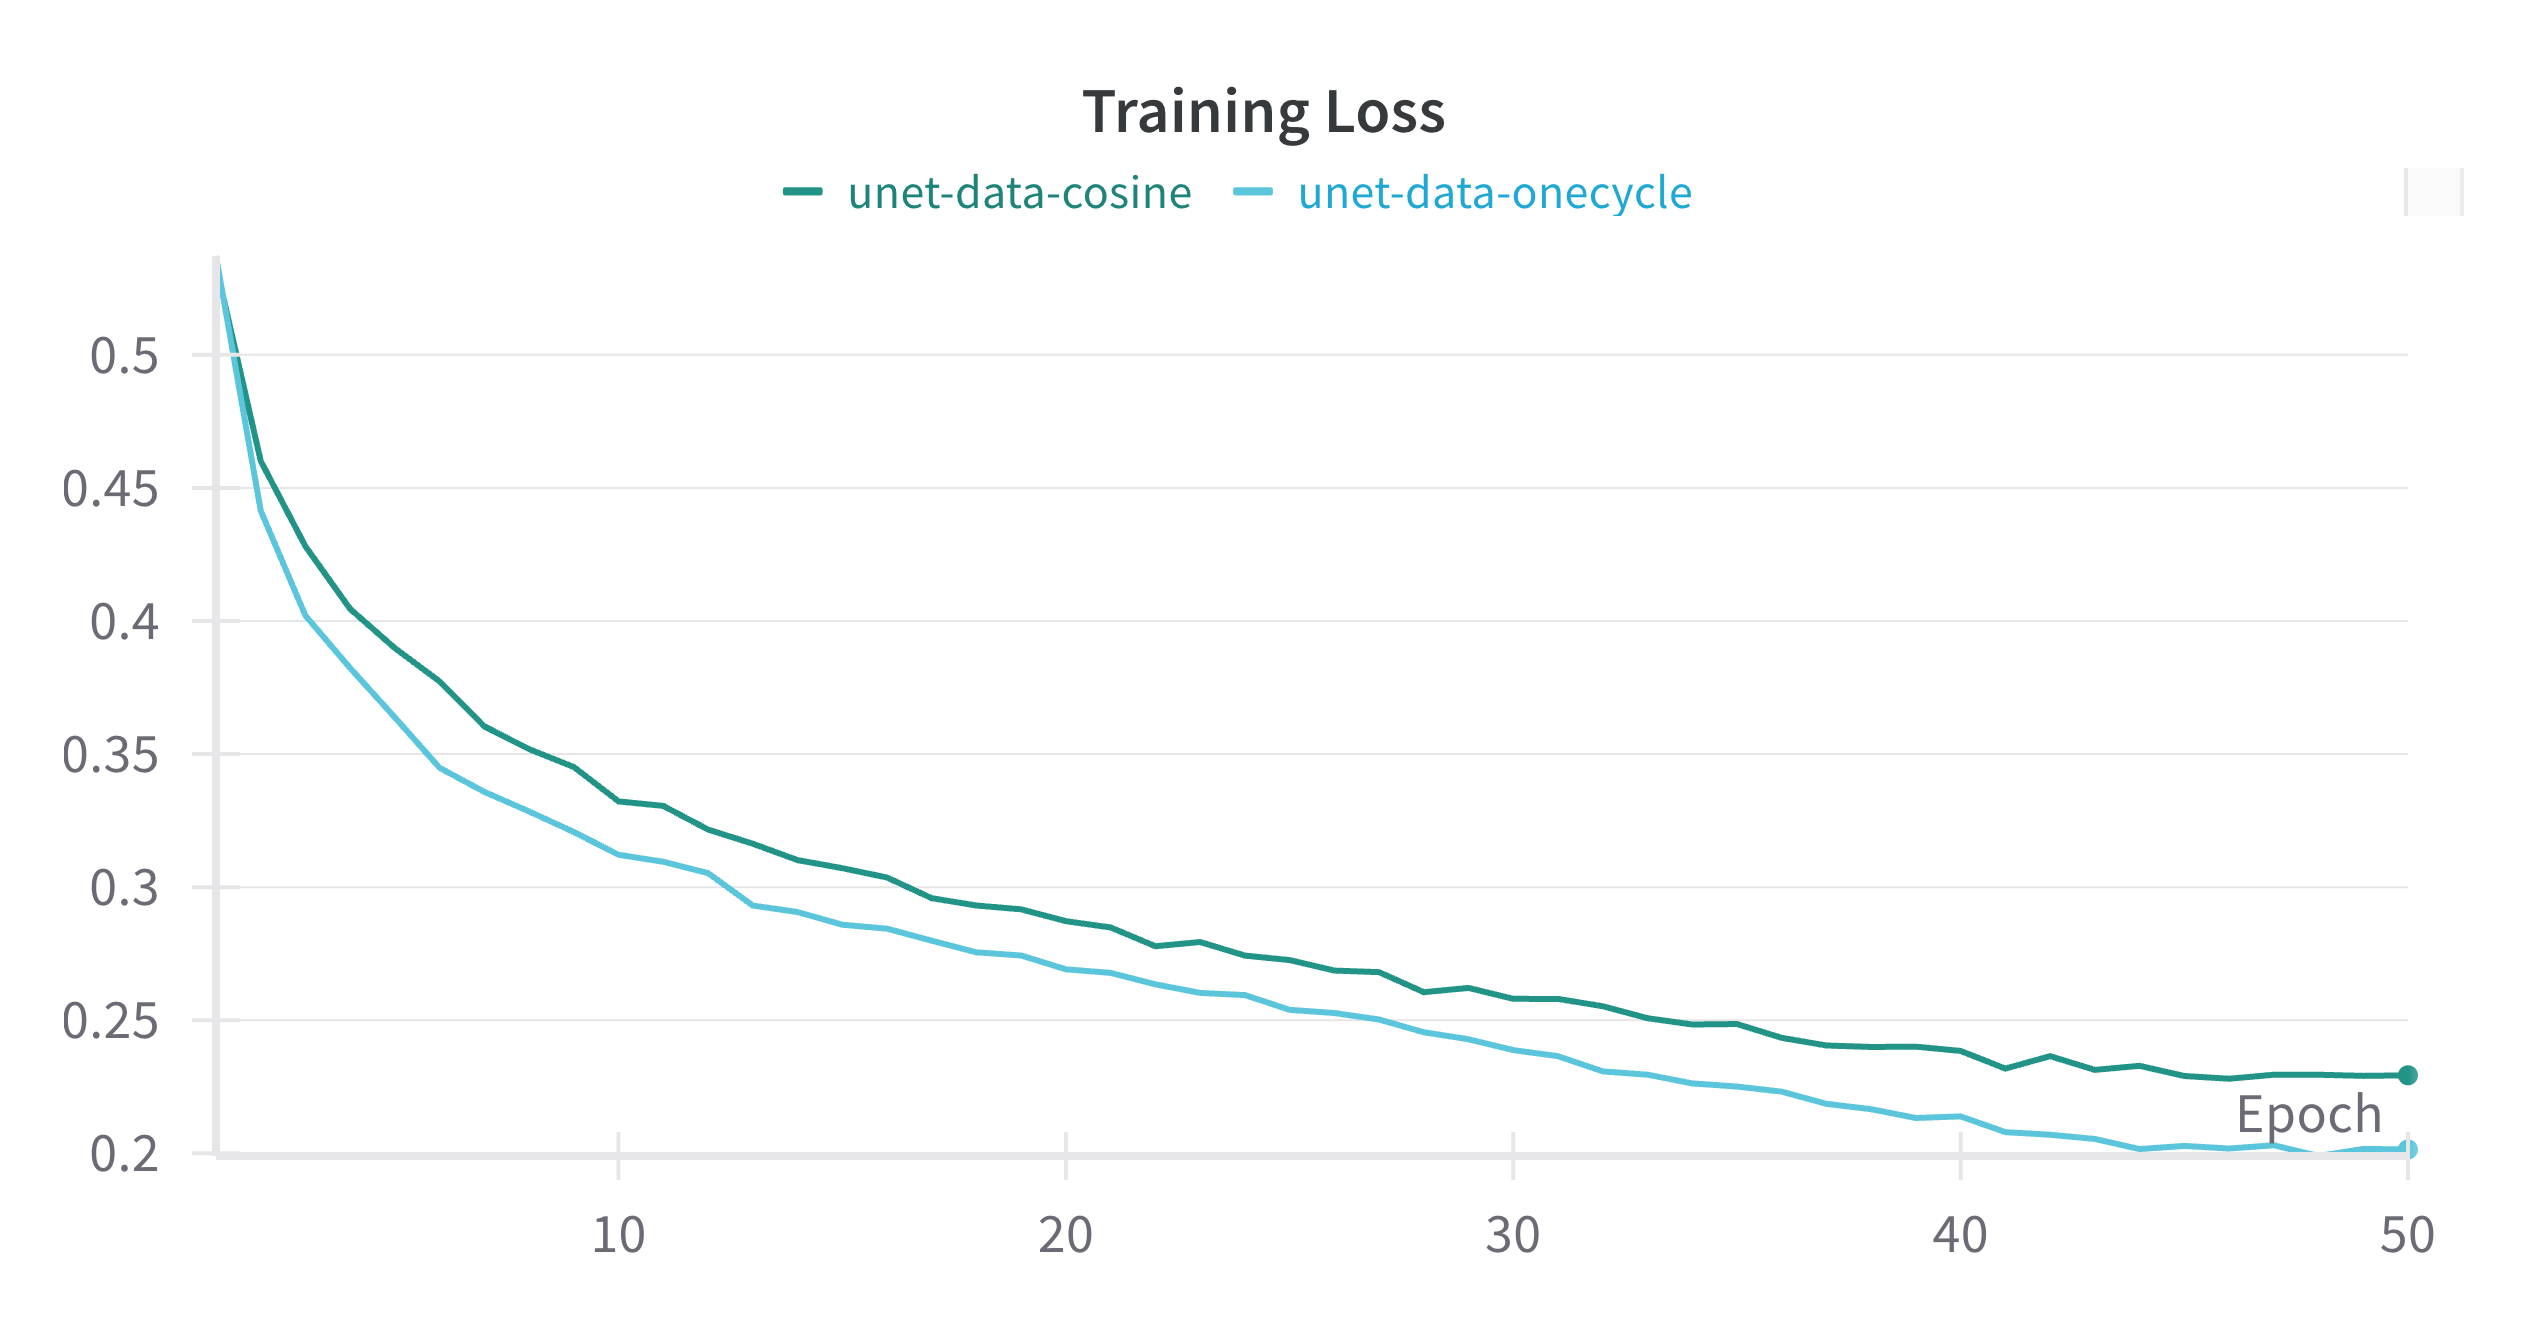
\includegraphics[width=0.95\linewidth]{figs/lr_unet_train_loss}
\caption{\textbf{Training loss over epochs for U-Net models.} \texttt{unet-data-cosine} uses the CosineAnnealingLR scheduler, while \texttt{unet-data-onecycle} uses the OneCycleLR scheduler. The OneCycleLR approach achieves lower training loss, particularly in the later stages of training.}
\label{fig:lrunettrainloss}
\end{figure}
\begin{figure}[H]
\centering
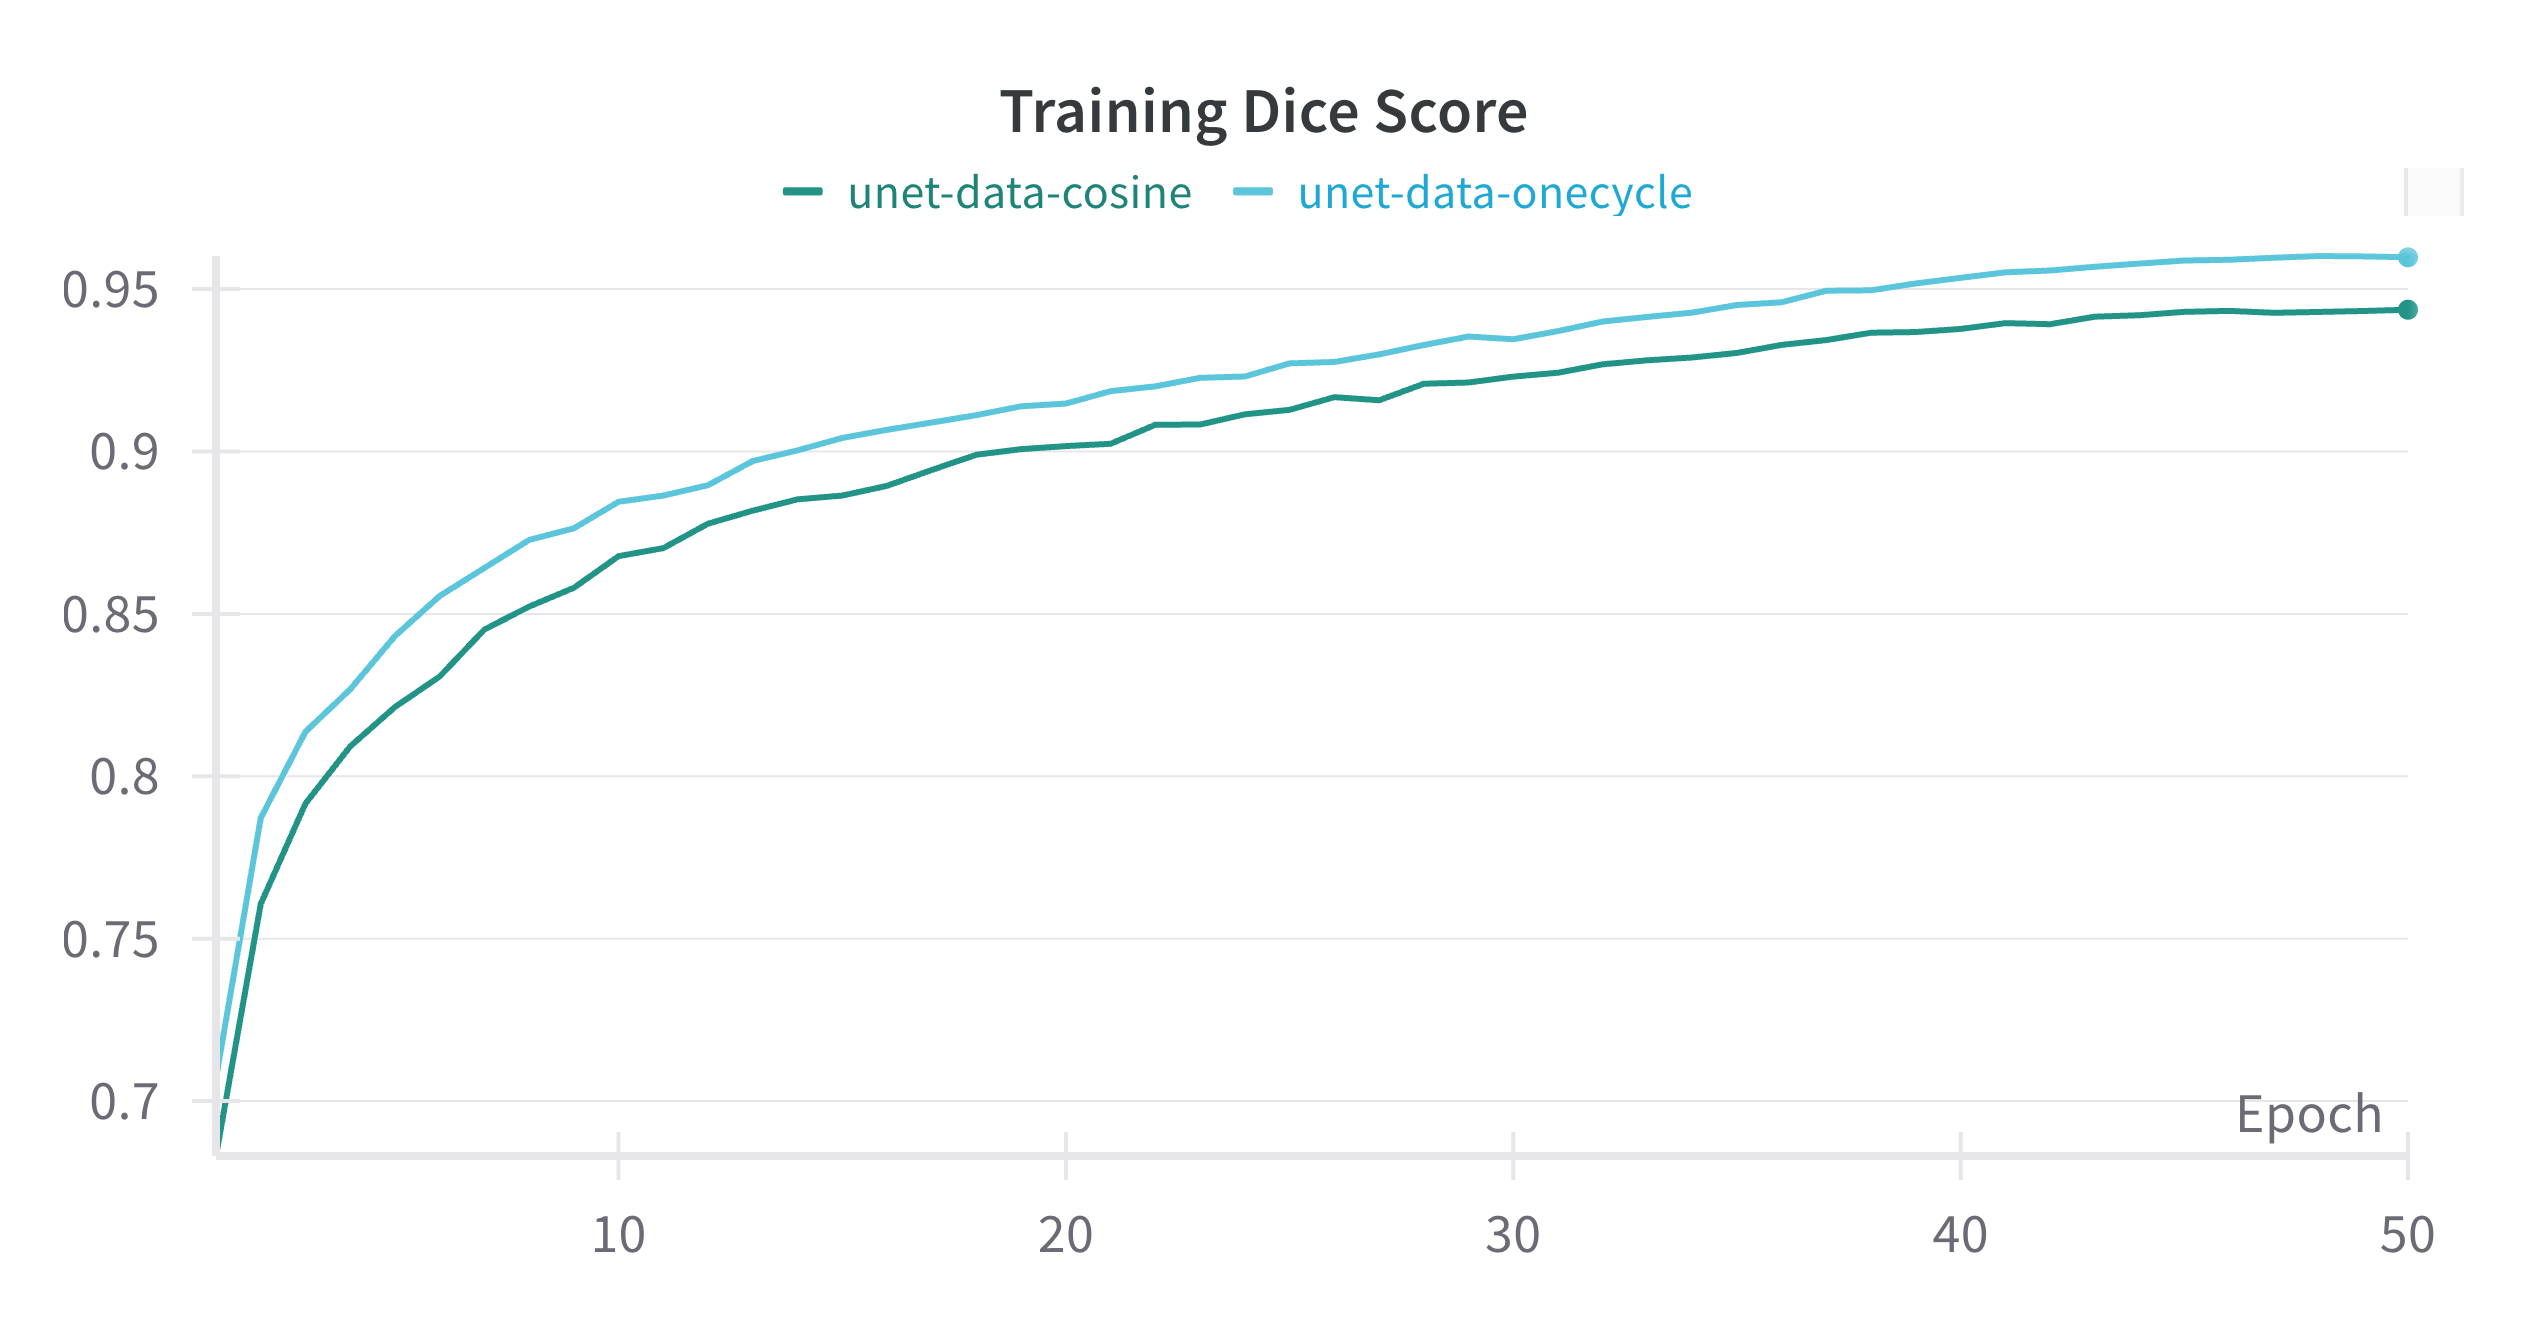
\includegraphics[width=0.95\linewidth]{figs/lr_unet_train_dice}
\caption{\textbf{Training Dice score over epochs for U-Net models.} \texttt{unet-data-cosine} uses the CosineAnnealingLR scheduler, while \texttt{unet-data-onecycle} uses the OneCycleLR scheduler. The OneCycleLR scheduler enables the model to achieve higher training Dice scores.}
\label{fig:lrunettraindice}
\end{figure}
\begin{figure}[H]
\centering
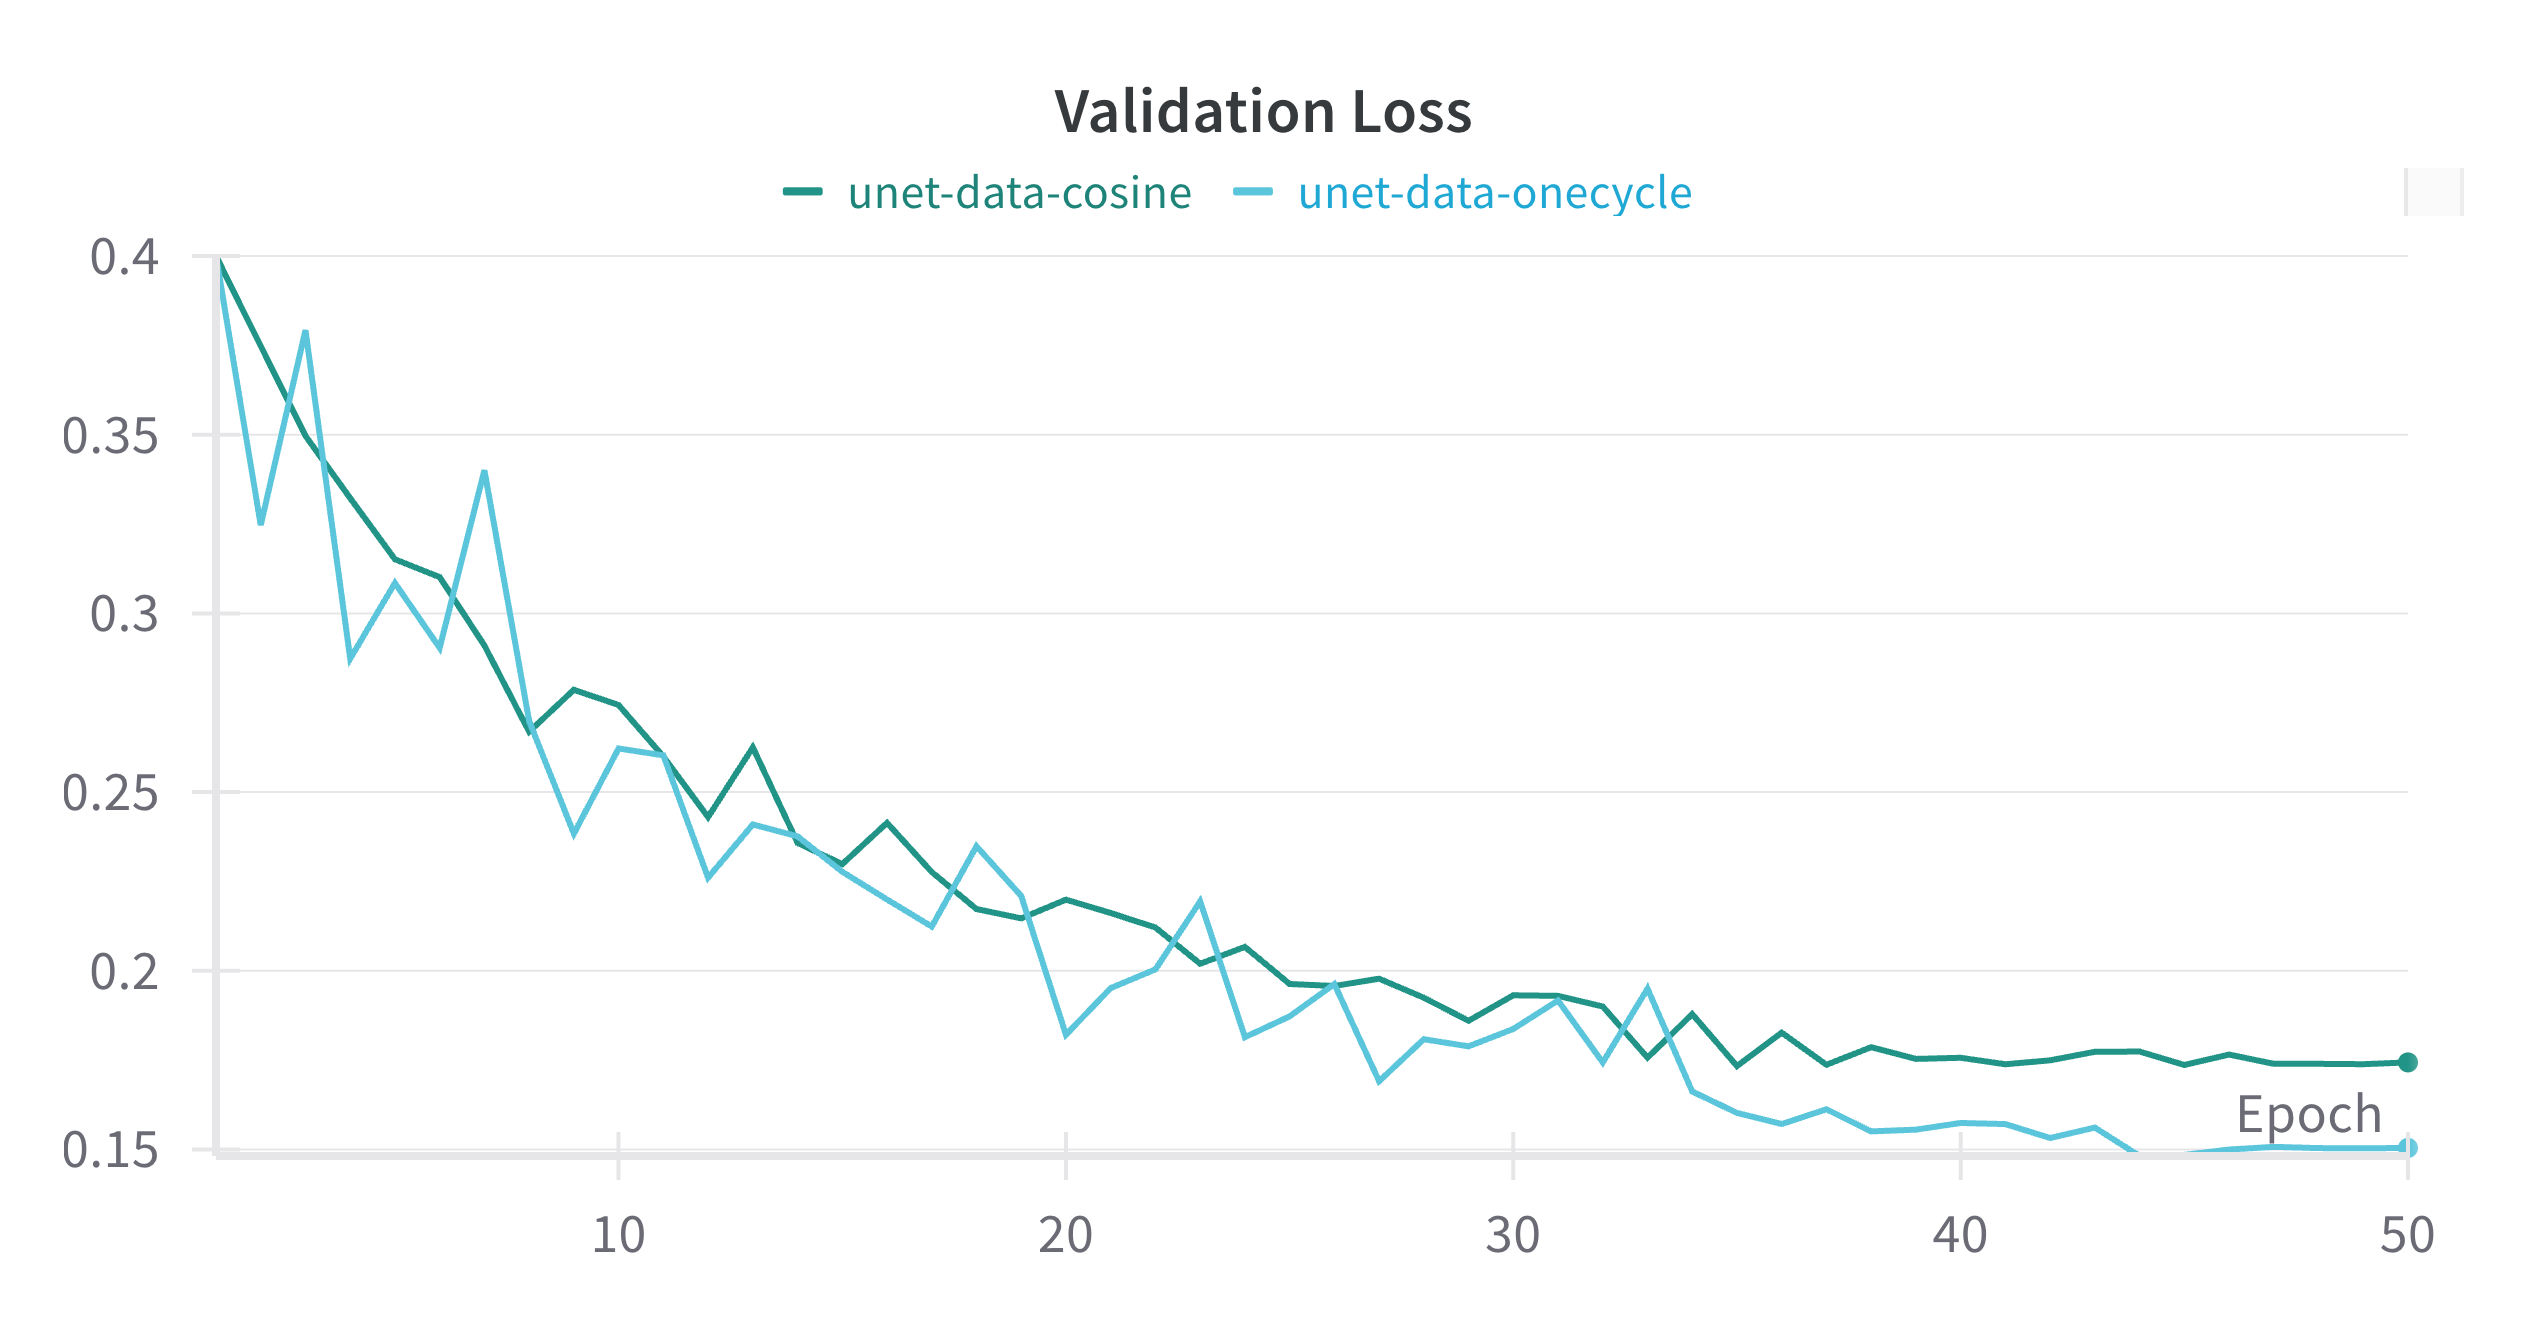
\includegraphics[width=0.95\linewidth]{figs/lr_unet_val_loss}
\caption{\textbf{Validation loss over epochs for U-Net models.} \texttt{unet-data-cosine} uses the CosineAnnealingLR scheduler, while \texttt{unet-data-onecycle} uses the OneCycleLR scheduler. The OneCycleLR approach maintains lower validation loss, indicating better generalization.}
\label{fig:lrunetvalloss}
\end{figure}
\begin{figure}[H]
\centering
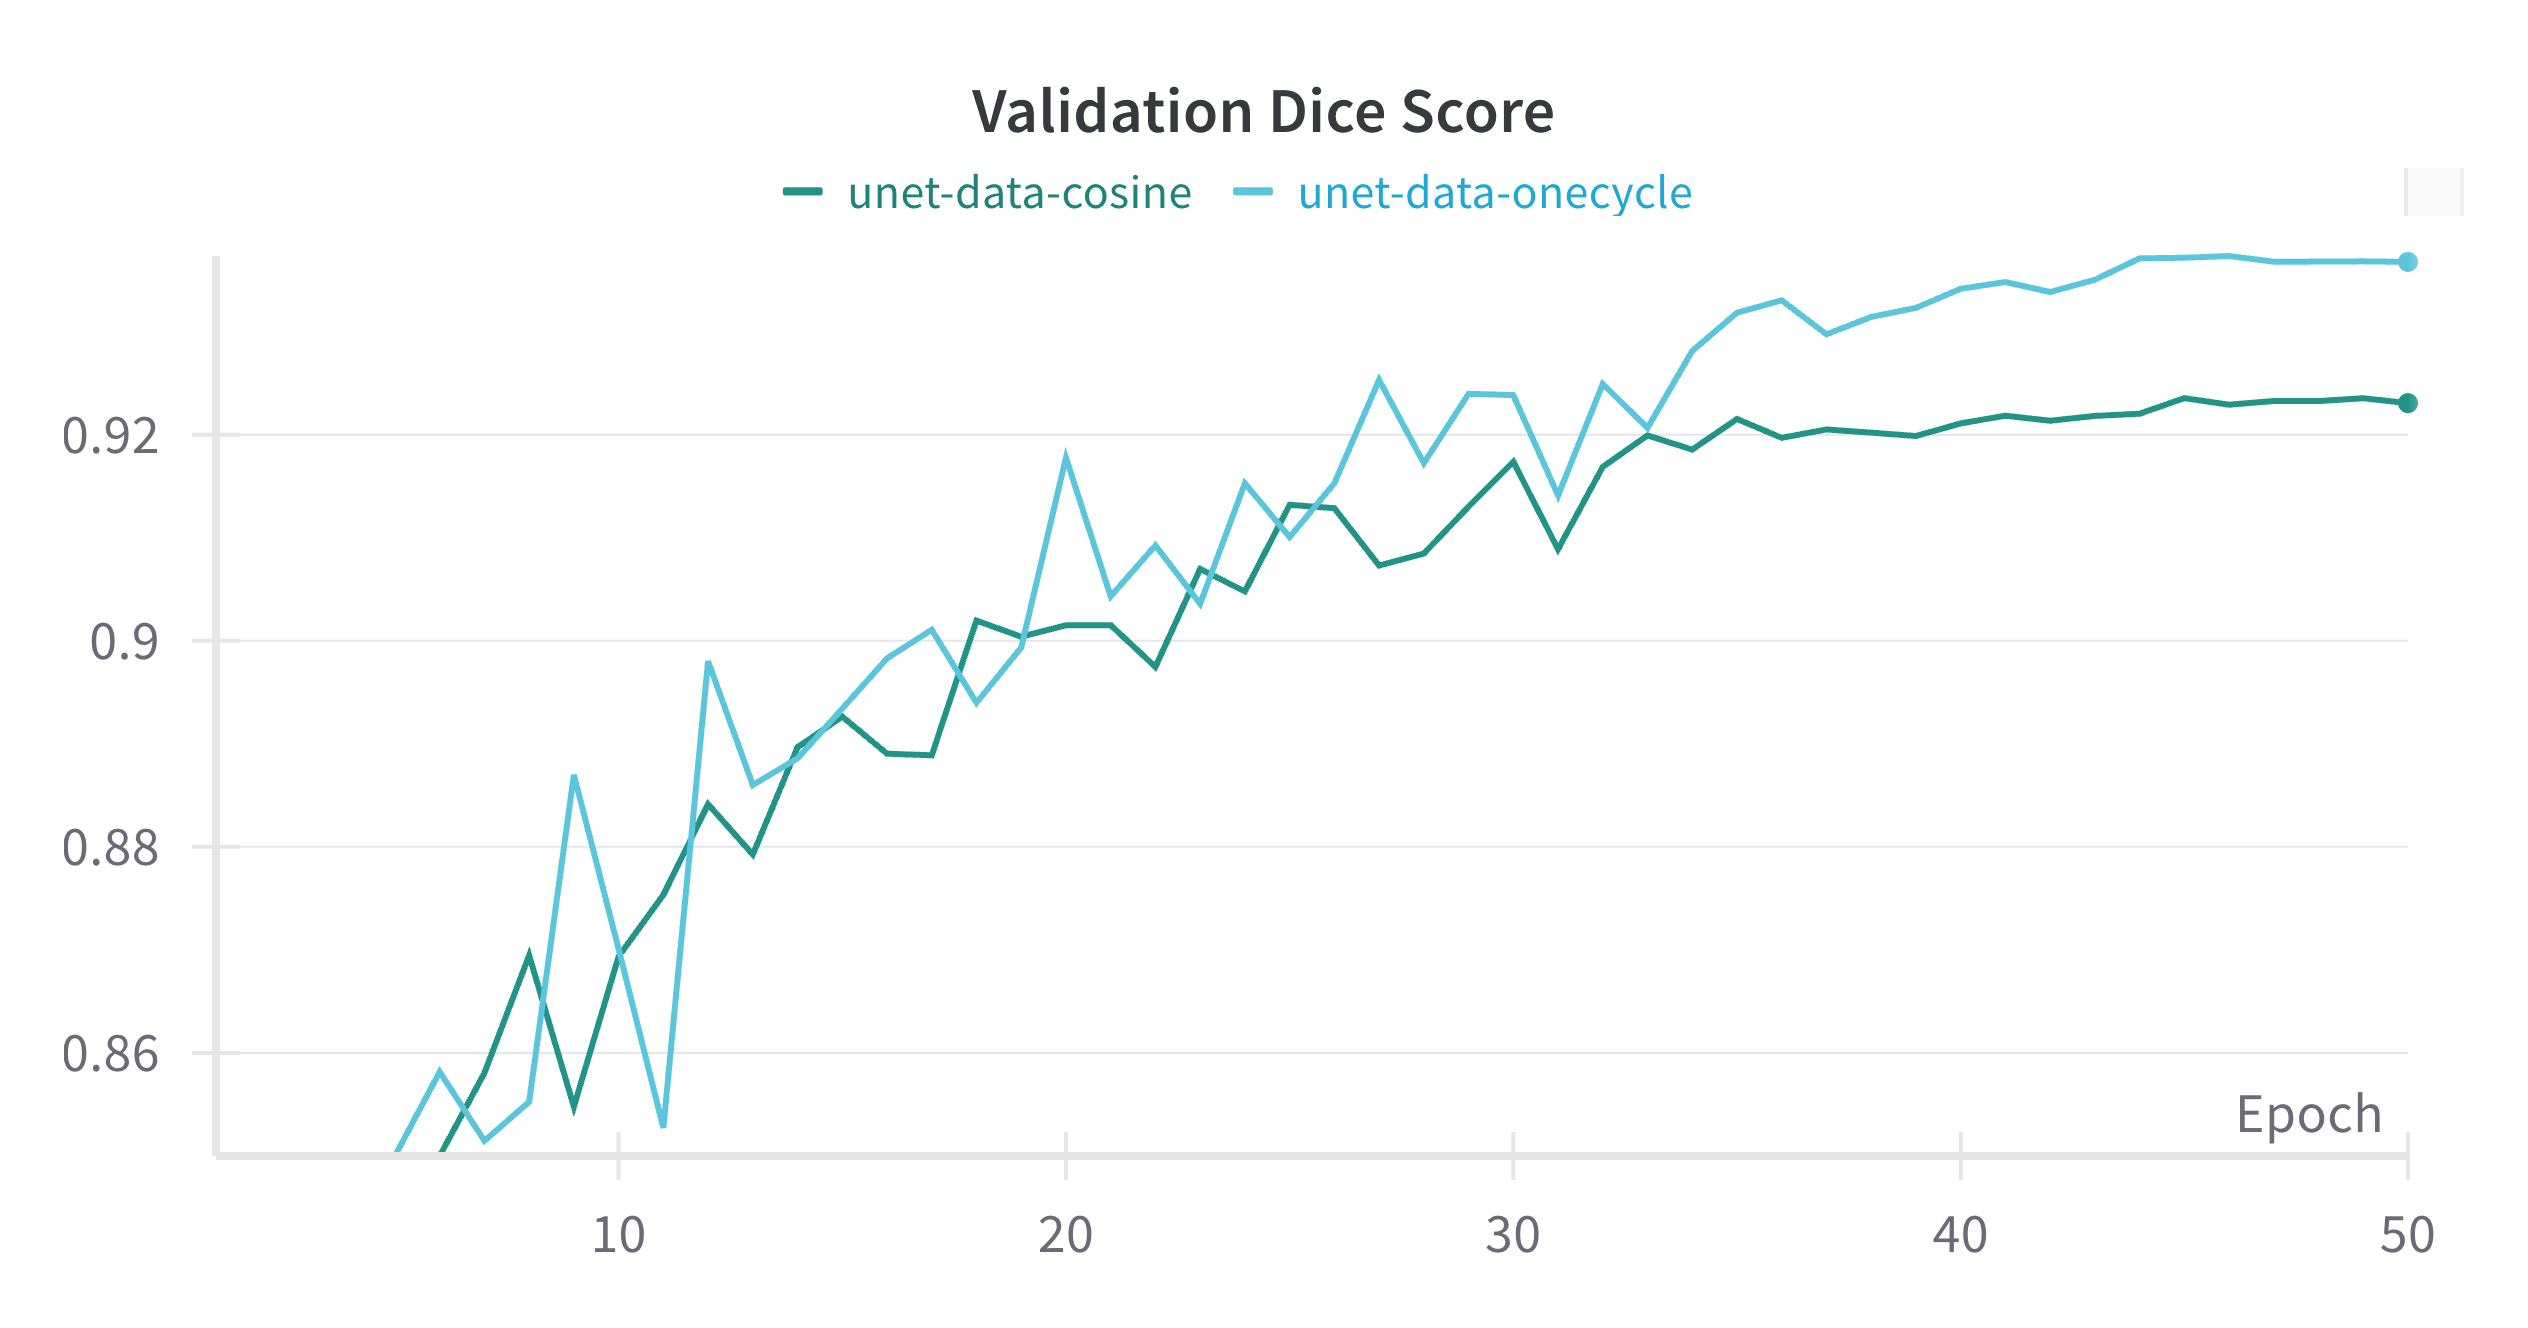
\includegraphics[width=0.95\linewidth]{figs/lr_unet_val_dice}
\caption{\textbf{Validation Dice score over epochs for U-Net models.} \texttt{unet-data-cosine} uses the CosineAnnealingLR scheduler, while \texttt{unet-data-onecycle} uses the OneCycleLR scheduler. The OneCycleLR approach achieves consistently higher validation Dice scores throughout training.}
\label{fig:lrunetvaldice}
\end{figure}

\paragraph{ResNet34\_U-Net.} Similar trends emerge when applying these learning rate schedulers to the ResNet34\_U-Net architecture. As shown in \autoref{fig:lrresnetlr}, the learning rate patterns follow the same principles as with the U-Net model. The training loss in \autoref{fig:lrresnsettrainloss} shows that the OneCycleLR scheduler initially leads to higher losses during the warm-up phase, but quickly achieves lower training loss as the learning rate decreases. This is mirrored in the training Dice scores depicted in \autoref{fig:lrresnettraindice}, where the OneCycleLR model rapidly improves after the initial epochs.

The validation performance, as illustrated in \autoref{fig:lrresnetvalloss} and \autoref{fig:lrresnetvaldice}, demonstrates that the OneCycleLR approach produces a model with better generalization capabilities. The validation loss is consistently lower, and the validation Dice score is higher for the model trained with OneCycleLR.

\begin{figure}[H]
\centering
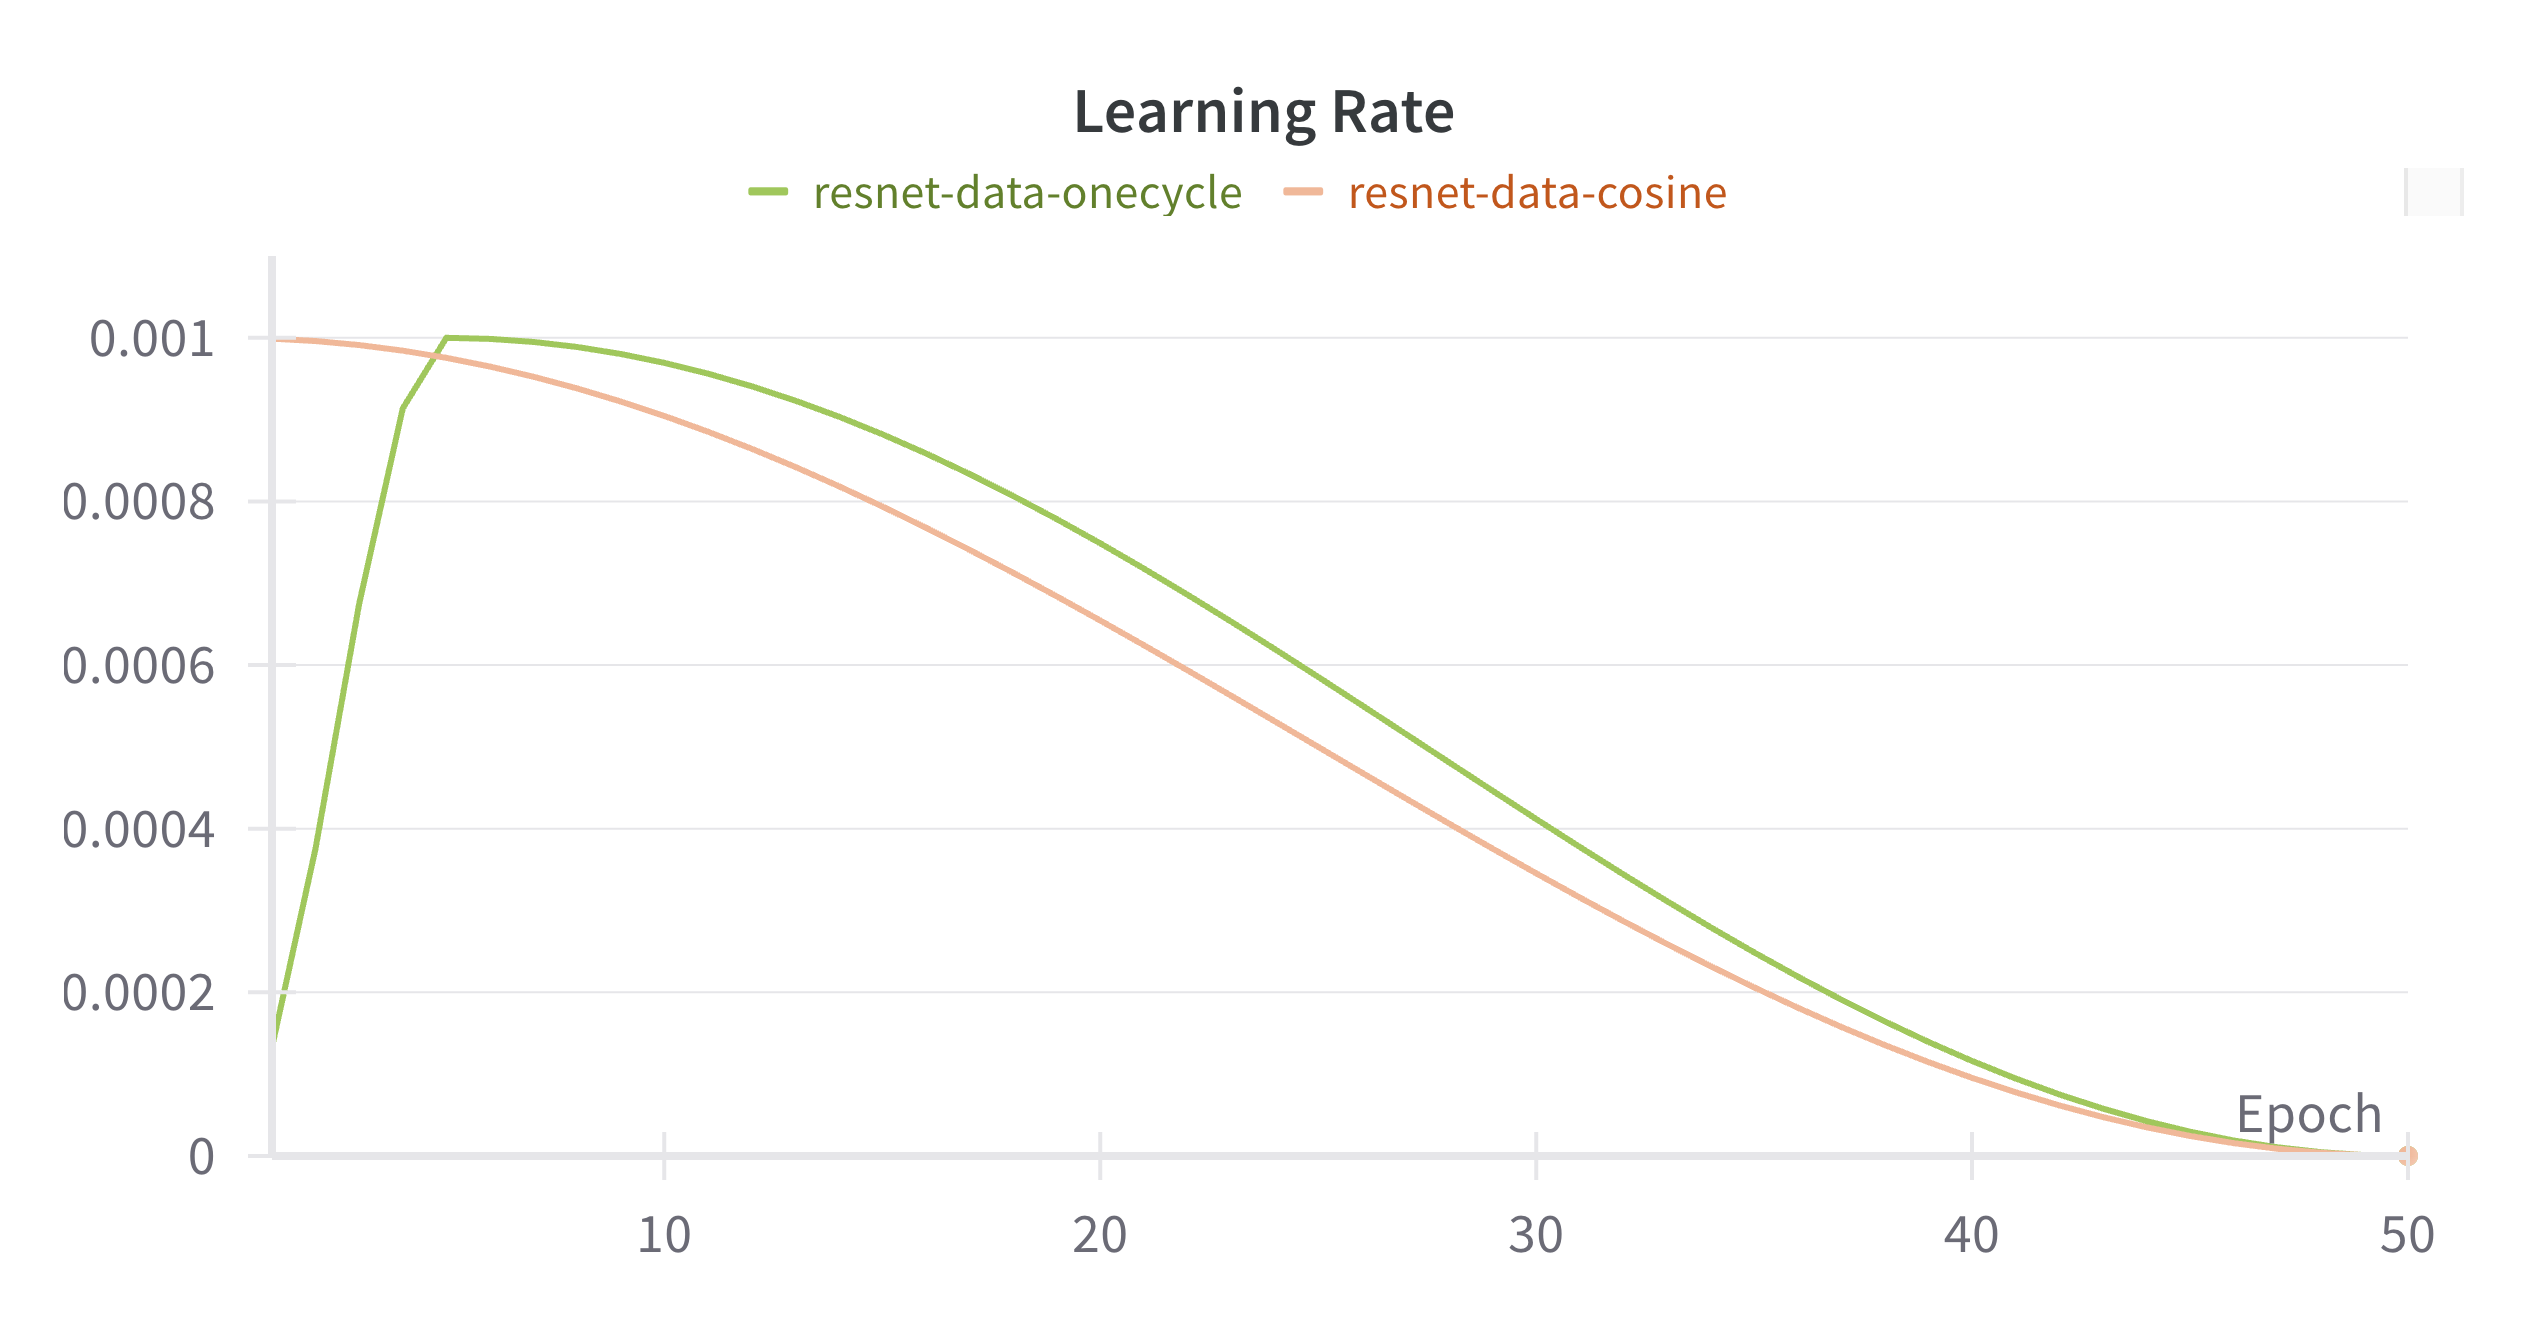
\includegraphics[width=0.95\linewidth]{figs/lr_resnet_lr}
\caption{\textbf{Learning rate over epochs for ResNet34\_U-Net models.} \texttt{resnet-data-cosine} uses the CosineAnnealingLR scheduler, while \texttt{resnet-data-onecycle} uses the OneCycleLR scheduler, showing the characteristic warm-up and cool-down phases.}
\label{fig:lrresnetlr}
\end{figure}
\begin{figure}[H]
\centering
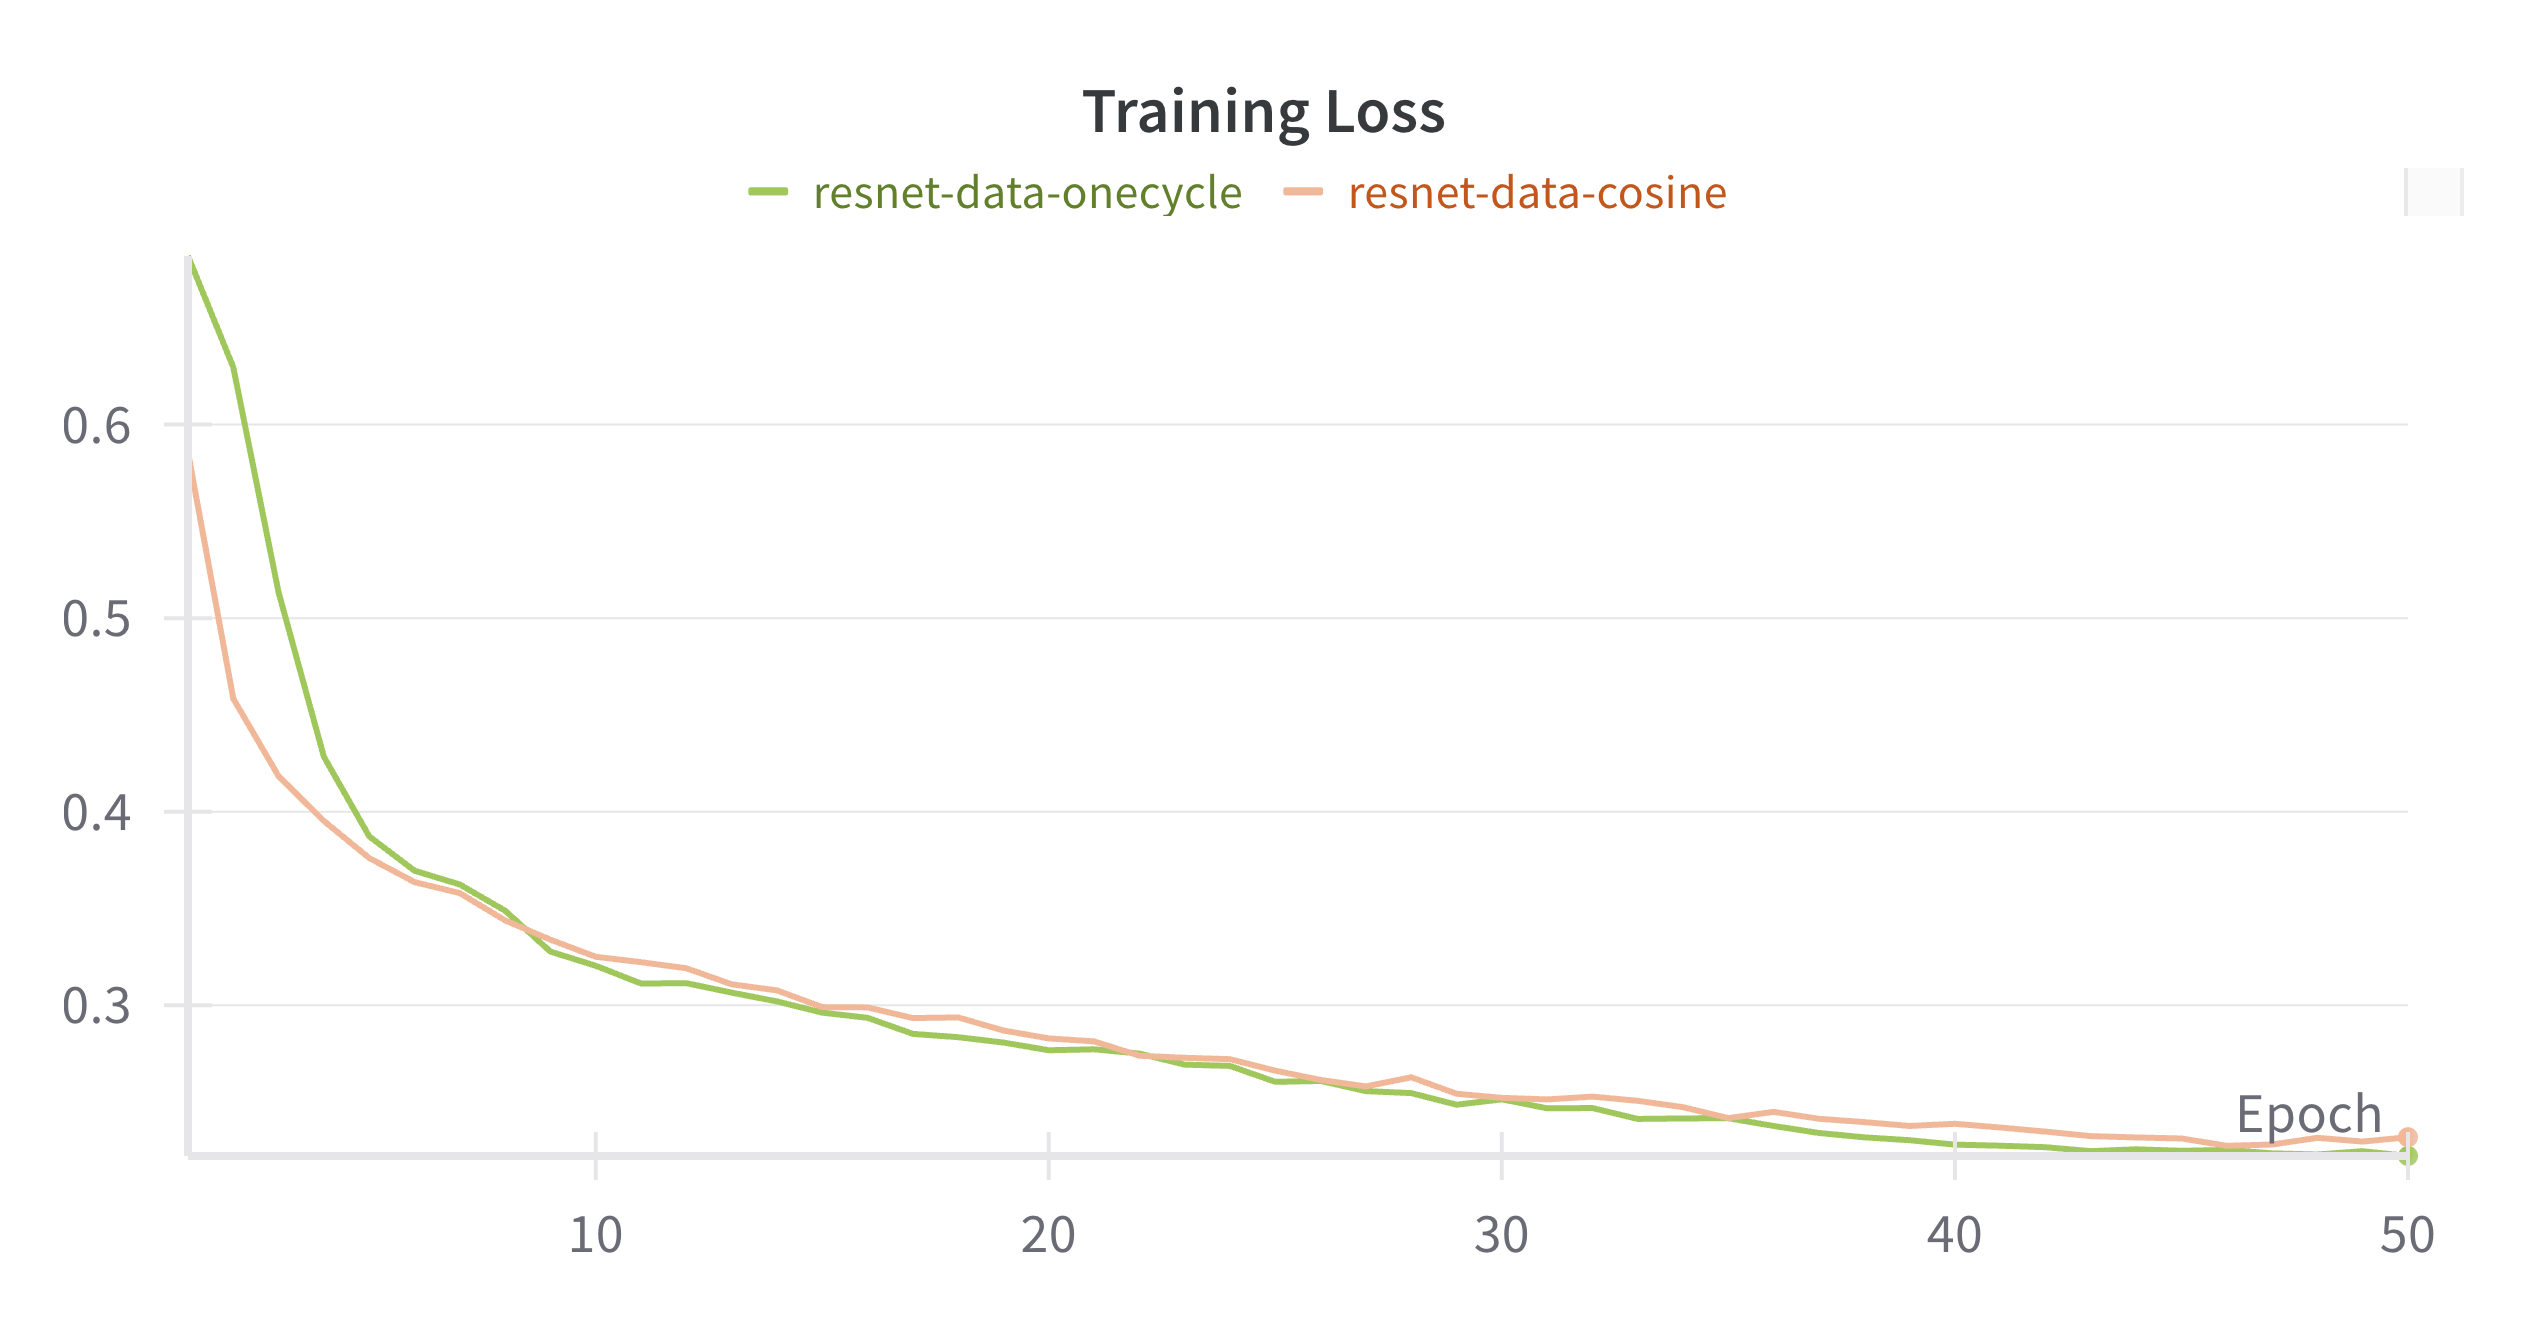
\includegraphics[width=0.95\linewidth]{figs/lr_resnset_train_loss}
\caption{\textbf{Training loss over epochs for ResNet34\_U-Net models.} \texttt{resnet-data-cosine} uses the CosineAnnealingLR scheduler, while \texttt{resnet-data-onecycle} uses the OneCycleLR scheduler. After the initial warm-up phase, the OneCycleLR approach achieves lower training loss.}
\label{fig:lrresnsettrainloss}
\end{figure}
\begin{figure}[H]
\centering
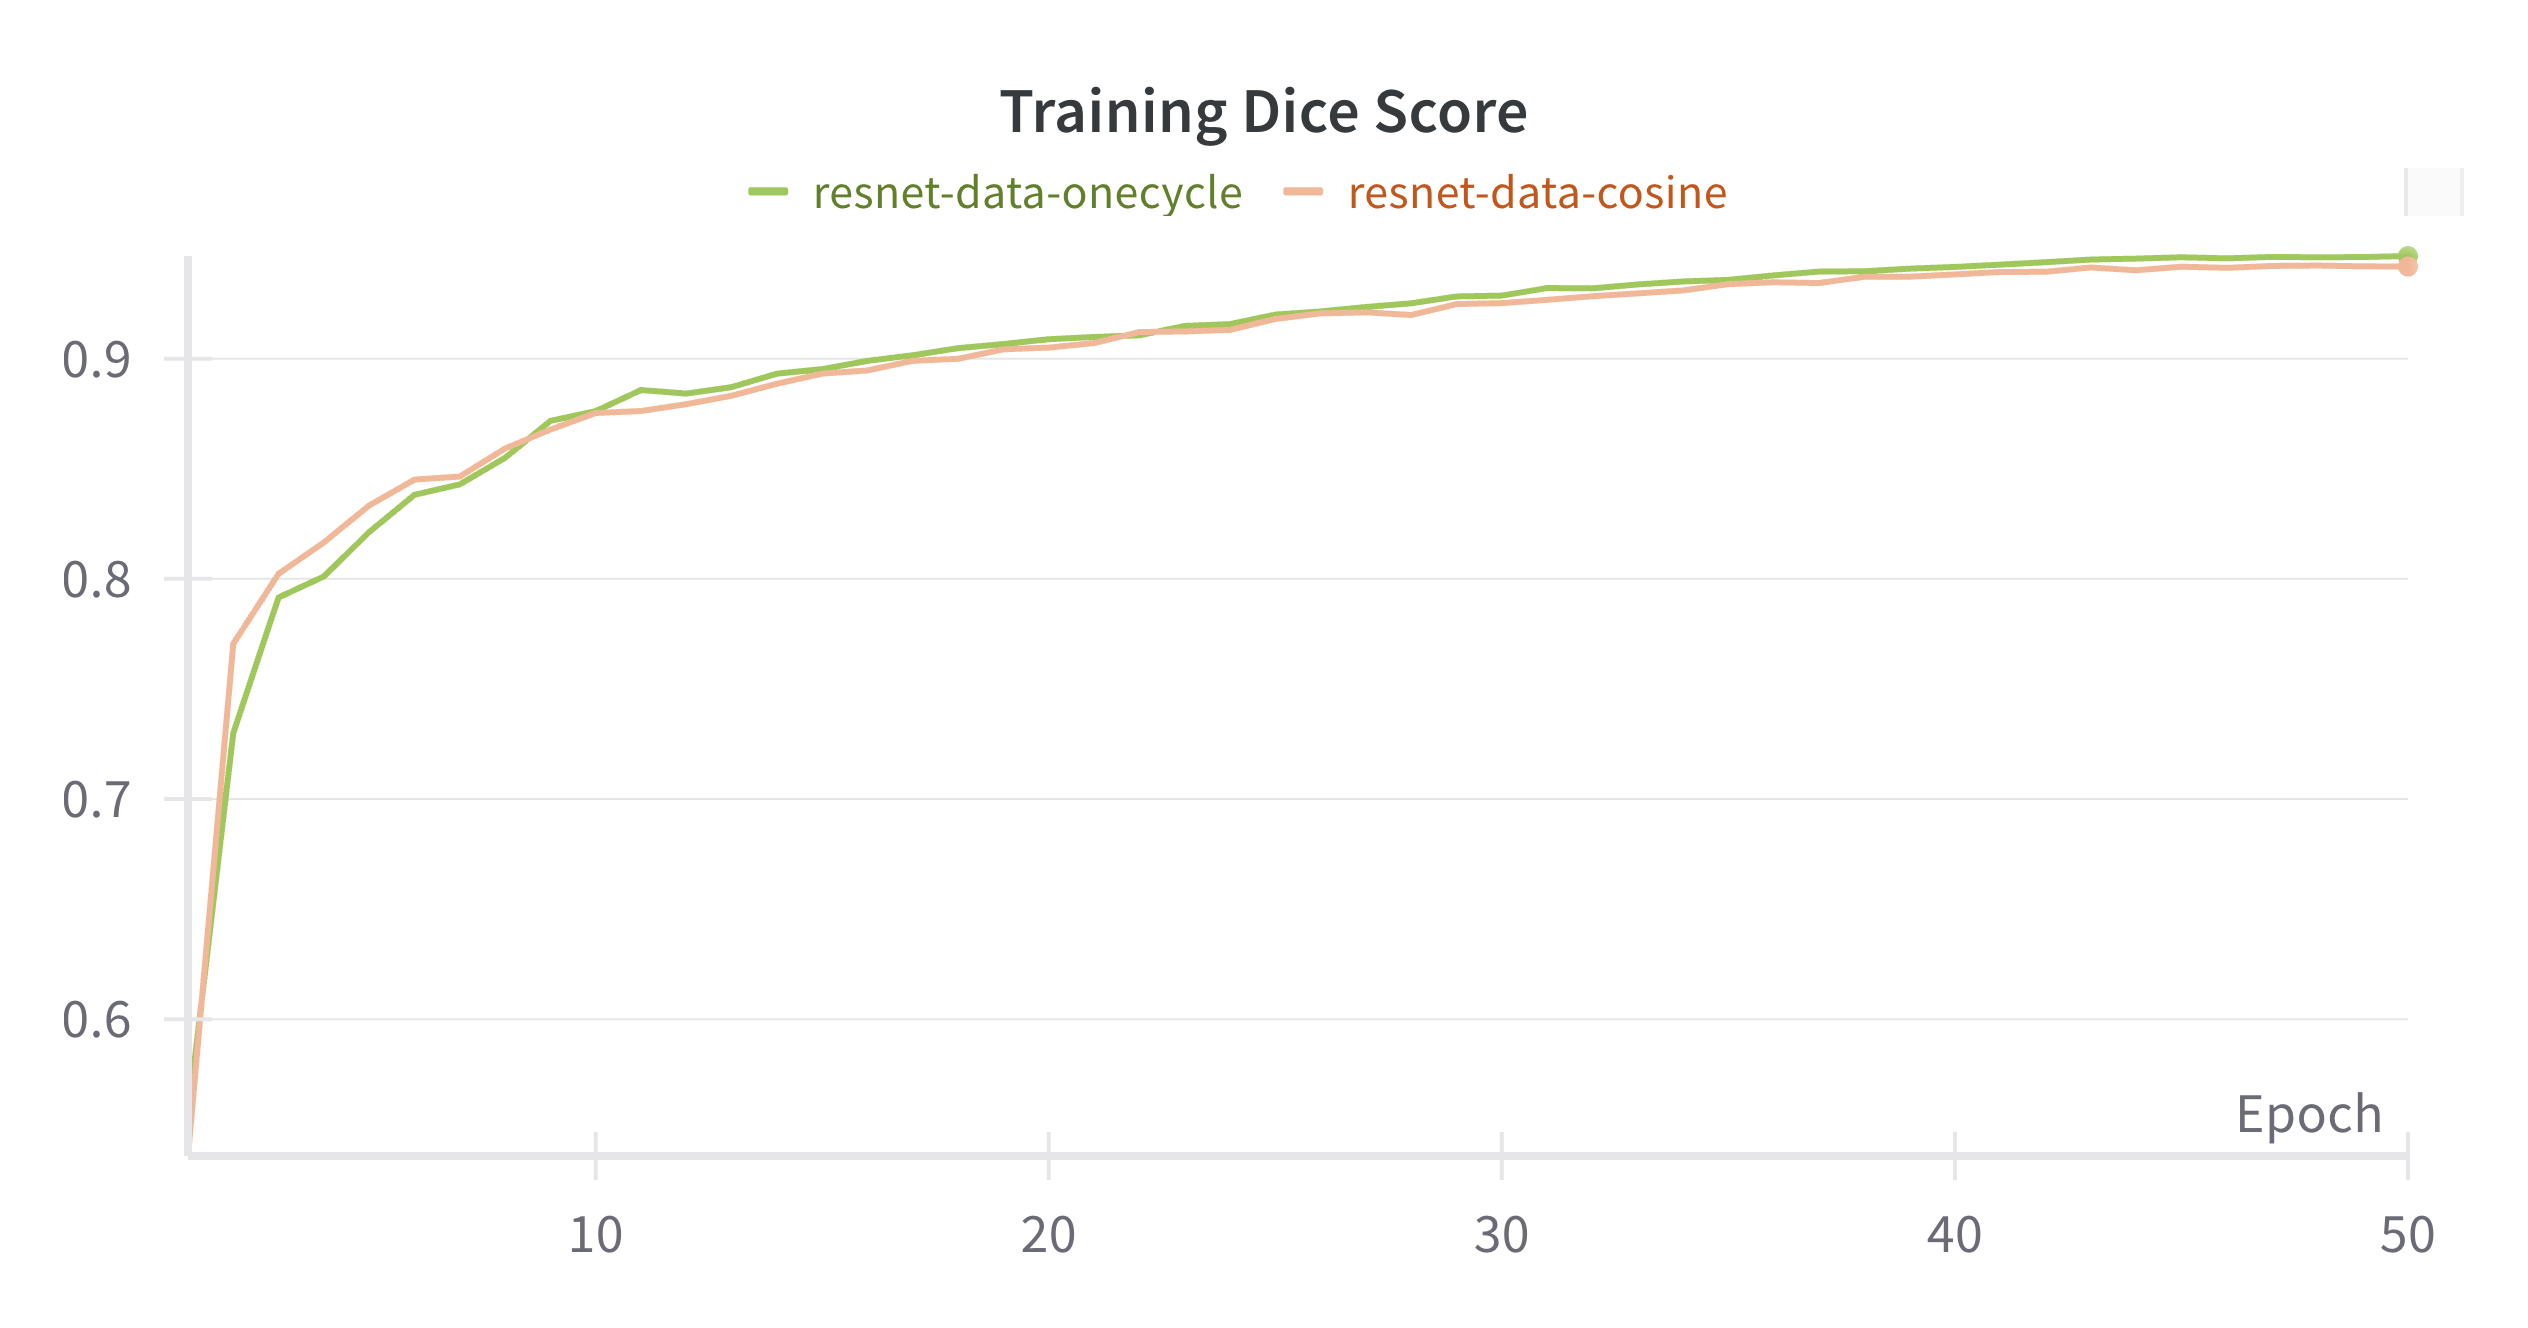
\includegraphics[width=0.95\linewidth]{figs/lr_resnet_train_dice}
\caption{\textbf{Training Dice score over epochs for ResNet34\_U-Net models.} \texttt{resnet-data-cosine} uses the CosineAnnealingLR scheduler, while \texttt{resnet-data-onecycle} uses the OneCycleLR scheduler. The OneCycleLR scheduler enables faster improvement in training Dice scores after the initial warm-up phase.}
\label{fig:lrresnettraindice}
\end{figure}
\begin{figure}[H]
\centering
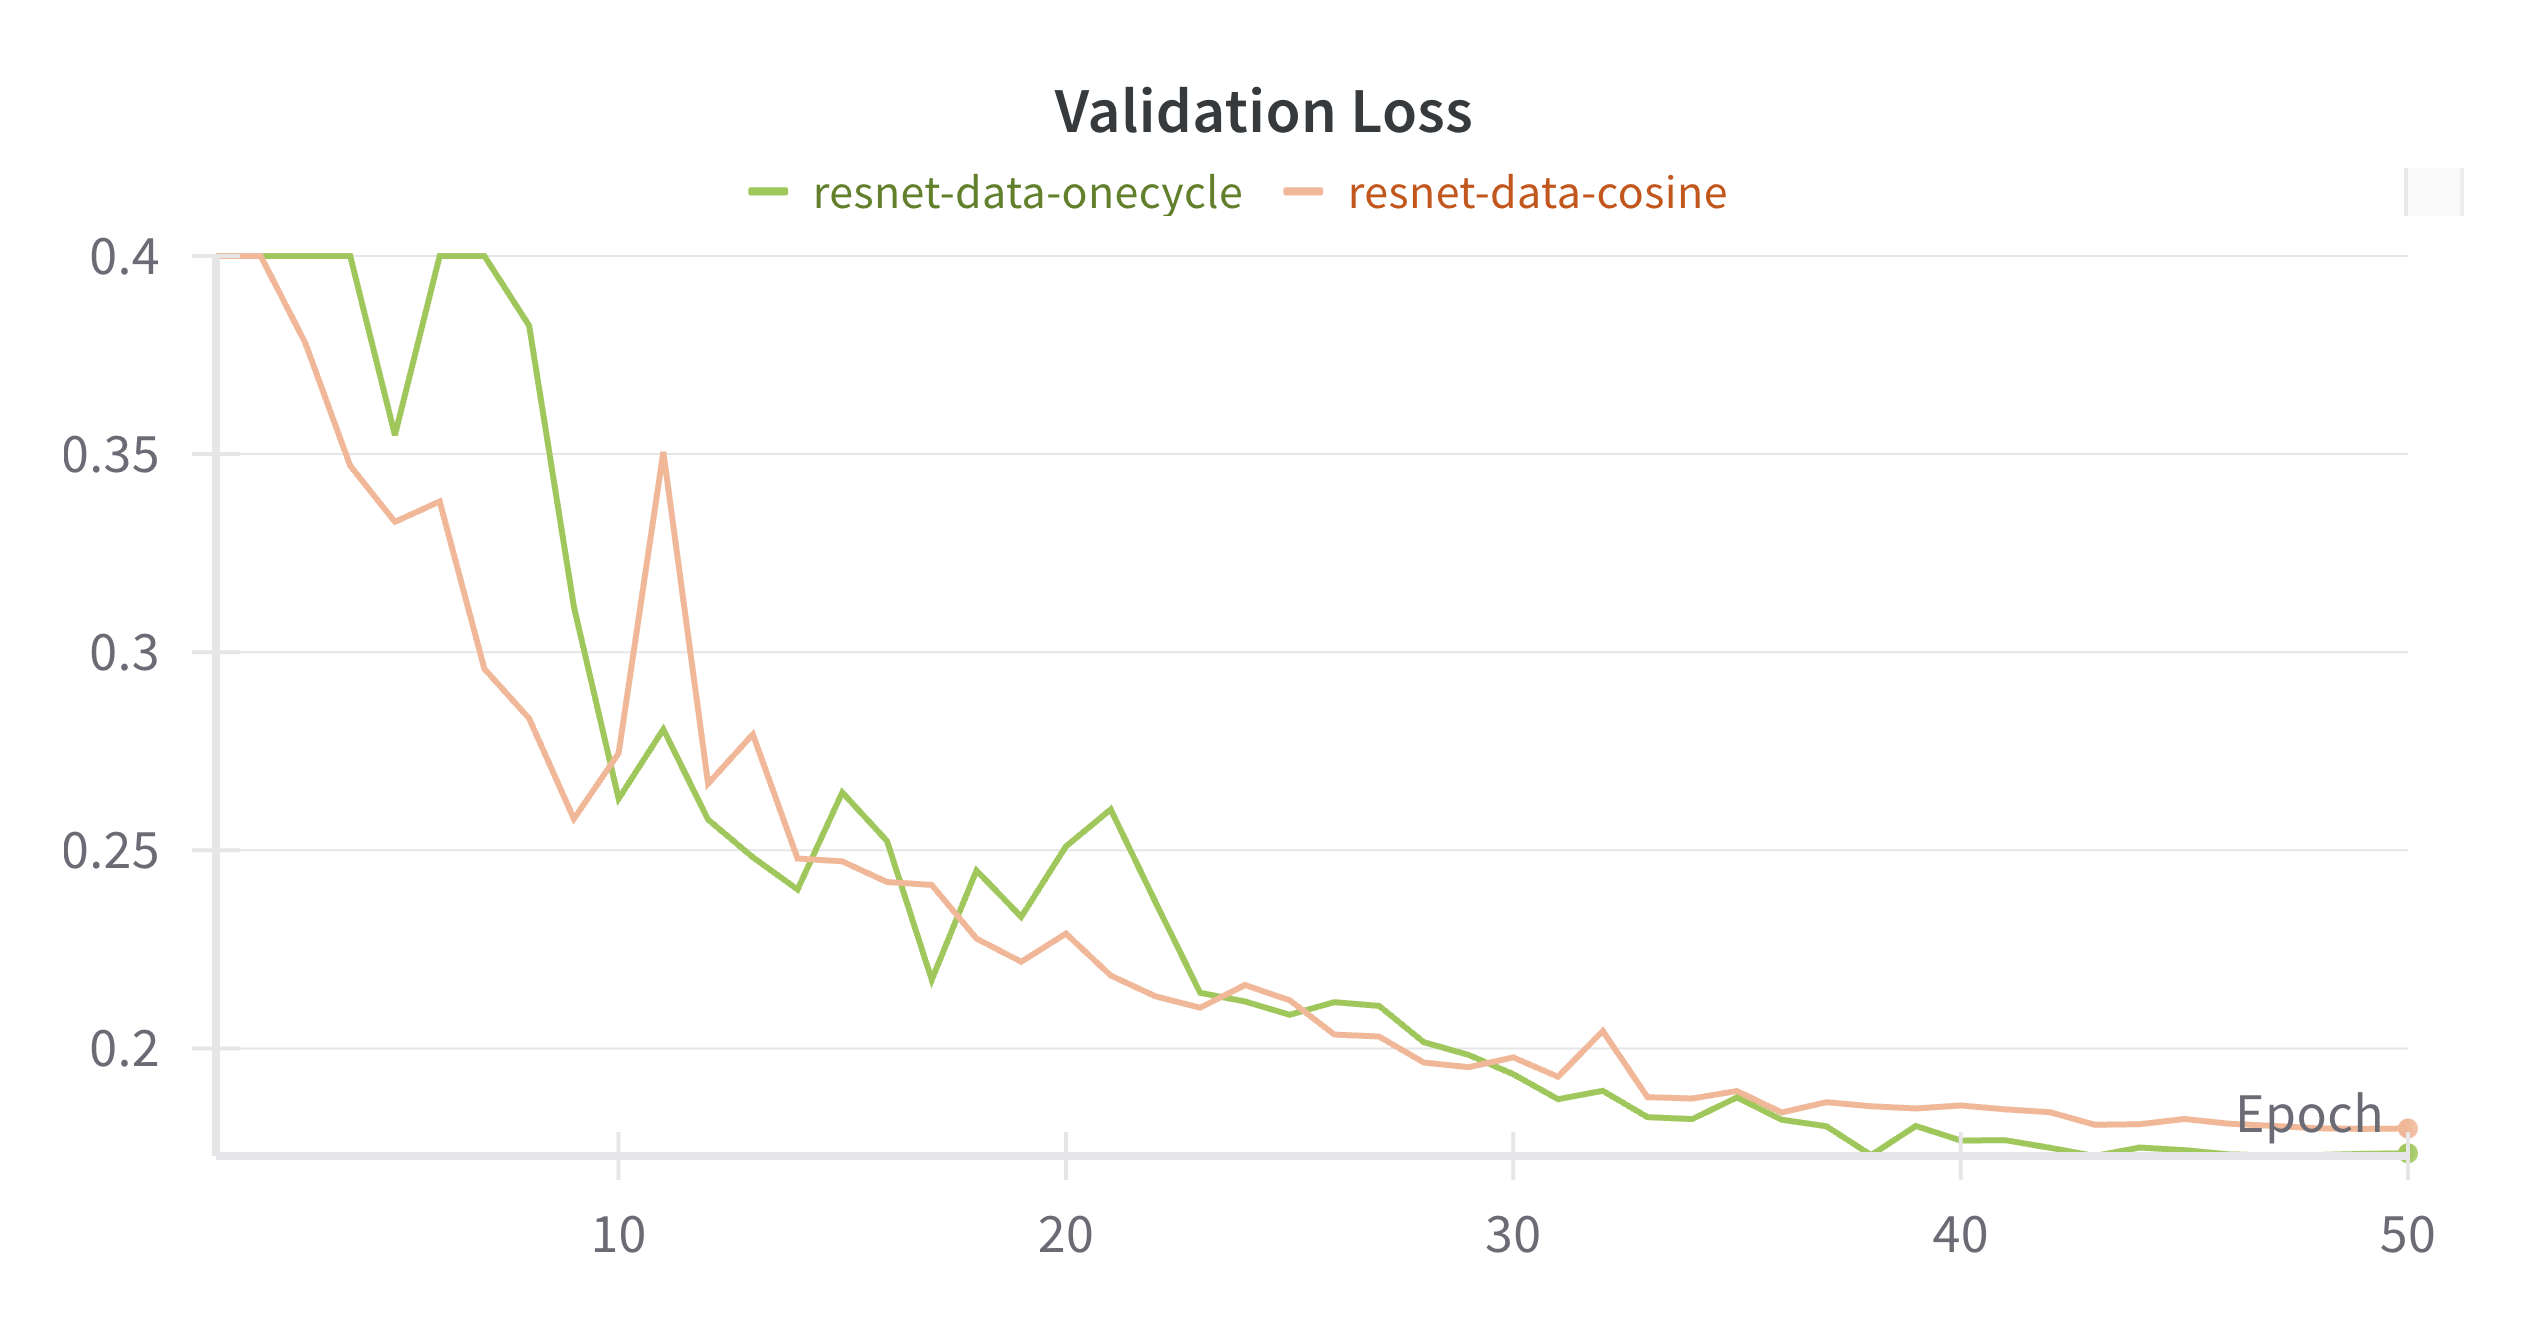
\includegraphics[width=0.95\linewidth]{figs/lr_resnet_val_loss}
\caption{\textbf{Validation loss over epochs for ResNet34\_U-Net models.} \texttt{resnet-data-cosine} uses the CosineAnnealingLR scheduler, while \texttt{resnet-data-onecycle} uses the OneCycleLR scheduler. The OneCycleLR approach maintains lower validation loss throughout most of the training process.}
\label{fig:lrresnetvalloss}
\end{figure}
\begin{figure}[H]
\centering
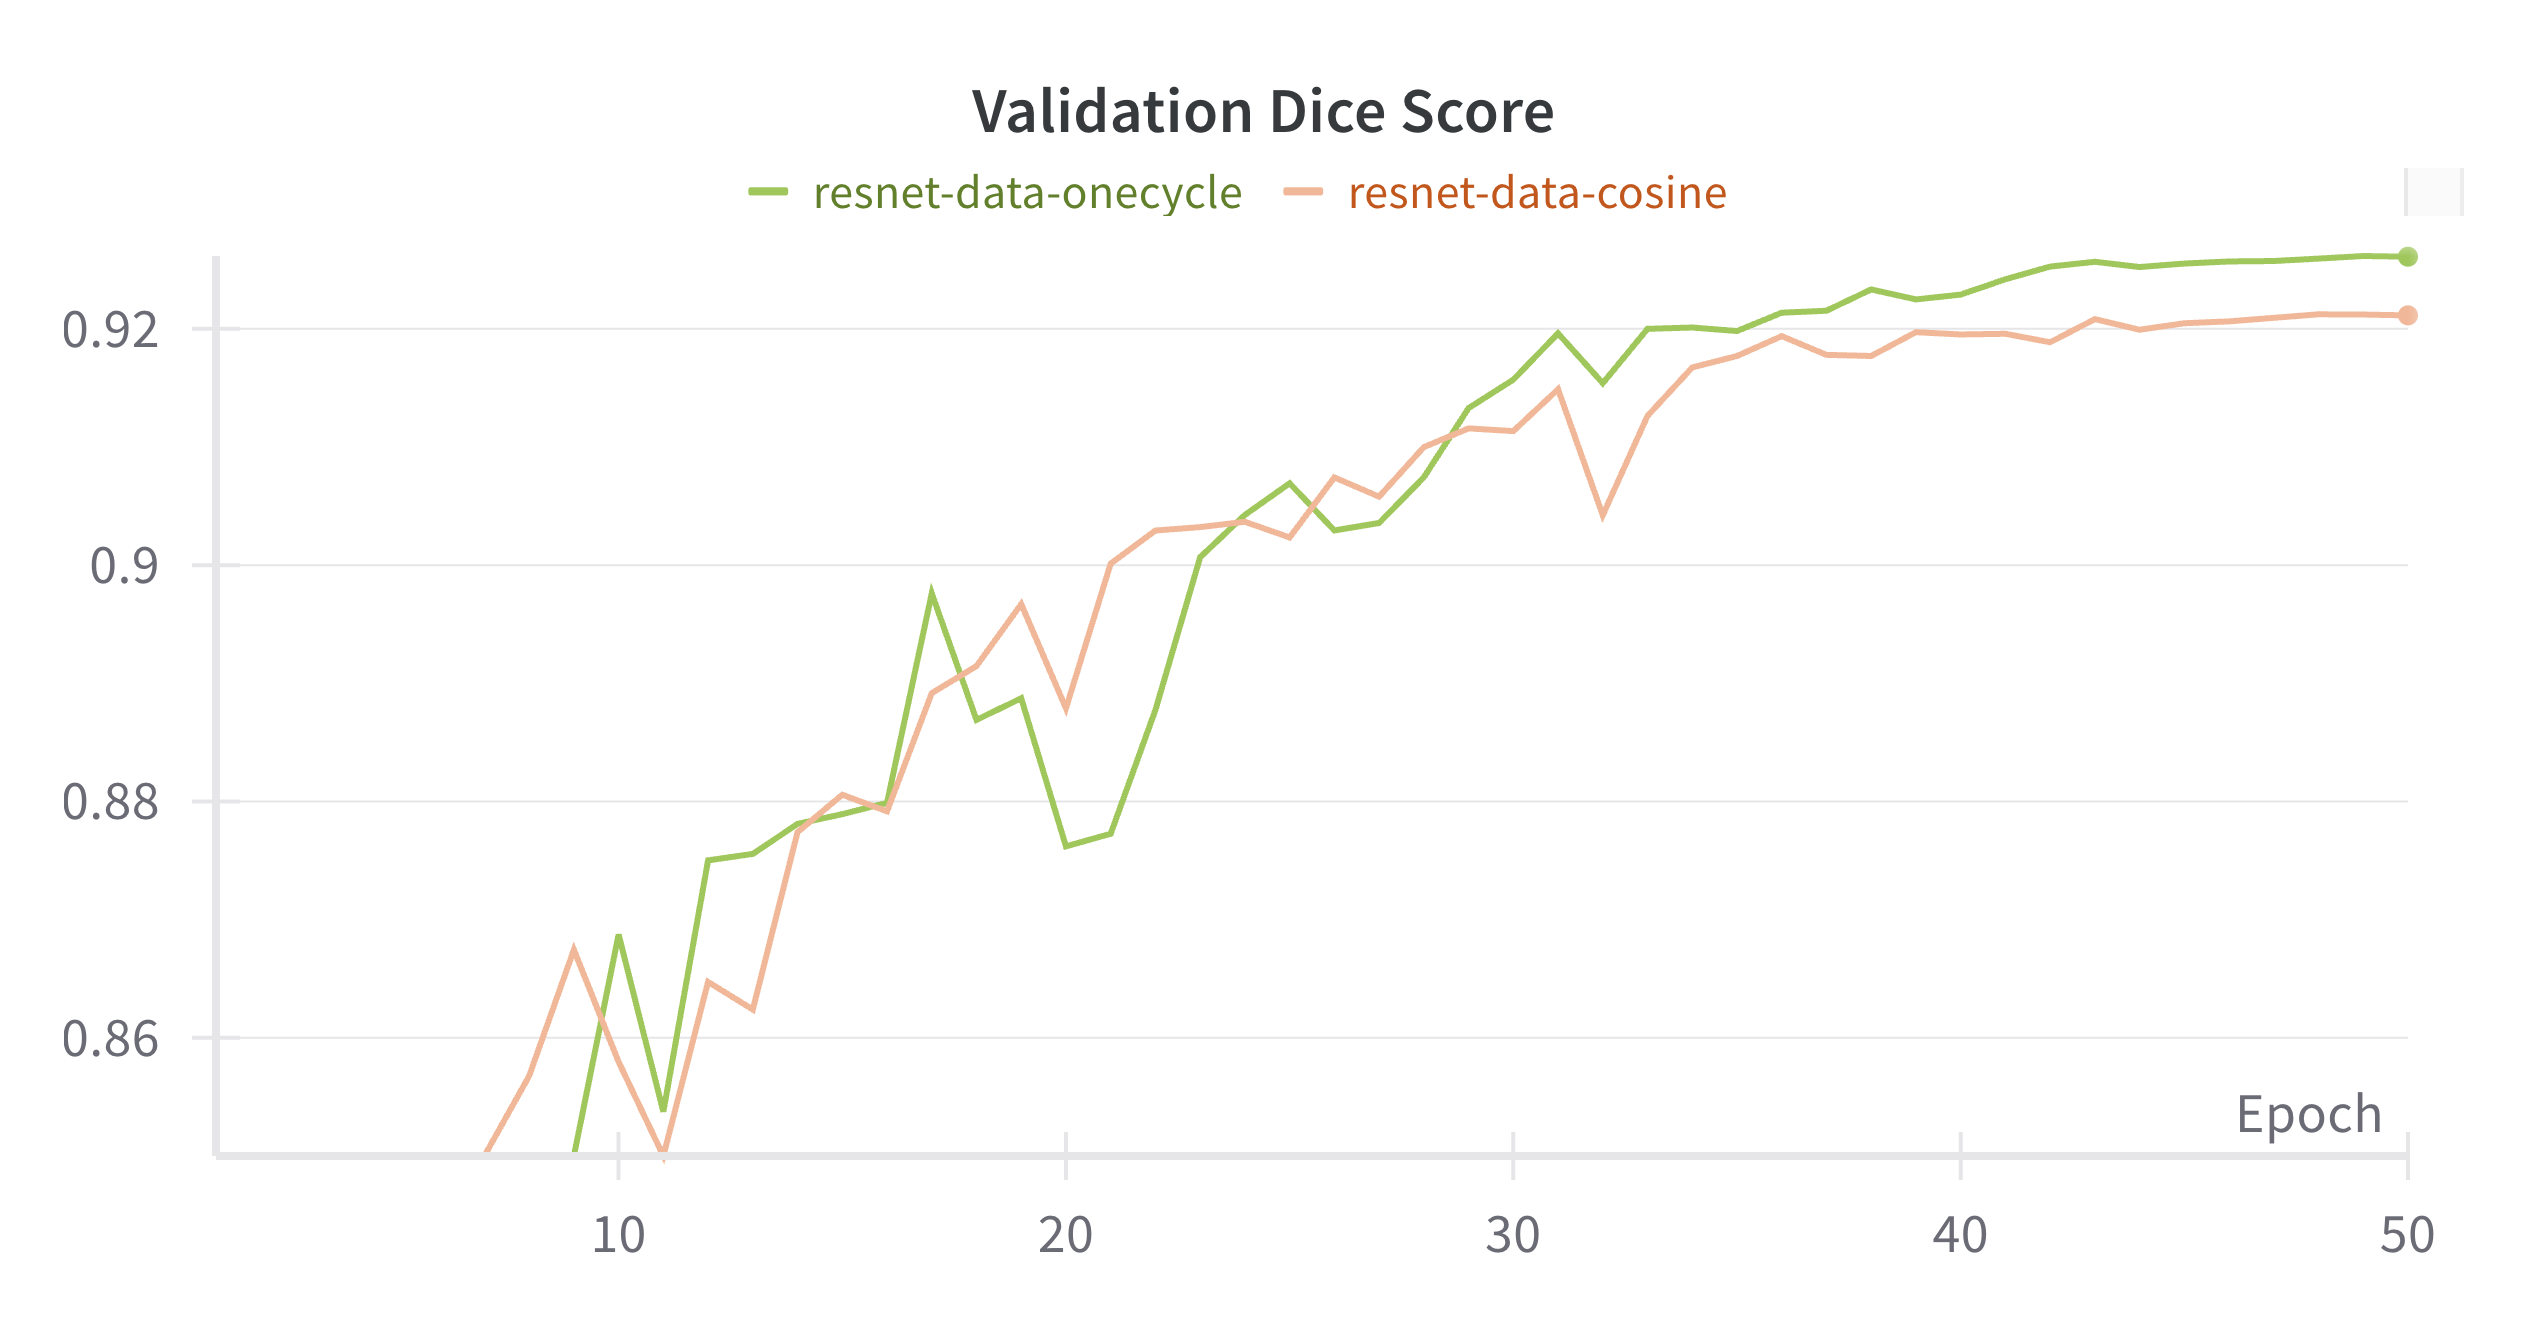
\includegraphics[width=0.95\linewidth]{figs/lr_resnet_val_dice}
\caption{\textbf{Validation Dice score over epochs for ResNet34\_U-Net models.} \texttt{resnet-data-cosine} uses the CosineAnnealingLR scheduler, while \texttt{resnet-data-onecycle} uses the OneCycleLR scheduler. The OneCycleLR approach demonstrates superior validation performance.}
\label{fig:lrresnetvaldice}
\end{figure}

These results consistently demonstrate that the OneCycleLR scheduler outperforms the CosineAnnealingLR scheduler for both architectures. The initial warm-up phase in OneCycleLR allows the models to explore the parameter space more effectively before gradually reducing the learning rate. This approach appears to help the models escape poor local minima early in training while still allowing for fine-tuning of weights in later epochs. The improvement is substantial, with OneCycleLR yielding approximately a 1\% increase in Dice score for U-Net. Based on these findings, we will use the OneCycleLR scheduler in all subsequent experiments to maximize model performance.


\subsection{Model architectures}
After establishing the optimal data preprocessing and training strategies, I conducted a comprehensive comparison of the U-Net and ResNet34\_U-Net architectures to determine their relative strengths in binary semantic segmentation. Both models were trained with identical hyperparameters: using data augmentation, the OneCycleLR scheduler, a base learning rate of 0.001, and training for 50 epochs.

Table \ref{tab:model_comparison} presents the detailed performance metrics of both architectures on the test set.
\begin{table}[h]
\centering
\caption{\textbf{Performance comparison of U-Net and ResNet34\_U-Net architectures.} Both models were trained with data augmentation, OneCycleLR scheduler, and identical hyperparameters.}
\label{tab:model_comparison}
\resizebox{0.95\linewidth}{!}{%
\begin{tabular}{lcc}
\toprule
\textbf{Metric} & \textbf{U-Net} & \textbf{ResNet34\_U-Net} \\
\midrule
Average Dice Score & 0.9291 & 0.9179 \\
Median Dice Score & 0.9528 & 0.9455 \\
Standard Deviation & 0.0842 & 0.0937 \\
Minimum Dice Score & 0.0000 & 0.0000 \\
Maximum Dice Score & 0.9982 & 0.9958 \\
Total Training Time (RTX 4090) & 30m & 16m \\
\bottomrule
\end{tabular}%
}
\end{table}

Interestingly, the U-Net architecture outperformed the more complex ResNet34\_U-Net across all accuracy metrics. The U-Net achieved a higher average Dice score (0.9291 vs. 0.9179) and median Dice score (0.9528 vs. 0.9455), while also demonstrating lower variability with a standard deviation of 0.0842 compared to 0.0937 for ResNet34\_U-Net. This suggests that the simpler U-Net architecture offers more consistent performance across the test dataset.

Both models struggled with certain challenging images, as evidenced by the minimum Dice score of 0.0000, indicating complete segmentation failure on at least one test sample. However, they both achieved excellent results on well-defined samples, with maximum Dice scores exceeding 0.99.

The superior performance of U-Net is somewhat surprising given that ResNet34\_U-Net incorporates residual connections, which typically aid in training deeper networks by mitigating gradient vanishing problems. However, for this particular dataset and binary segmentation task, the simpler U-Net architecture appears to be more effective. This could be attributed to several factors:

\begin{enumerate}
\item The Oxford-IIIT Pet Dataset may not be complex enough to benefit from the additional capacity of ResNet34\_U-Net.
\item The ResNet34 encoder's aggressive use of maxpooling and strided convolutions to rapidly reduce spatial dimensions likely causes loss of fine-grained spatial information that's crucial for precise boundary segmentation. While this design choice makes ResNet efficient for classification tasks, it can be detrimental for pixel-level segmentation where spatial precision is paramount.
\item The U-Net's more direct skip connections between corresponding encoder and decoder layers may preserve spatial information more effectively for this specific segmentation task.
\end{enumerate}

Despite the performance advantage of U-Net, it's worth noting that the ResNet34\_U-Net offers a significant computational efficiency benefit, with total training time approximately 47\% faster than the standard U-Net (16 minutes vs. 30 minutes for the complete 50-epoch training run on an RTX 4090). This efficiency stems from ResNet's design choices that reduce feature map sizes earlier in the network, resulting in fewer operations in the deeper layers.

These findings highlight that architectural complexity does not always translate to better performance, and that the standard U-Net remains a strong baseline for semantic segmentation tasks, particularly when properly trained with data augmentation and appropriate learning rate scheduling. However, in scenarios where computational resources or training time are limited, the ResNet34\_U-Net could be a reasonable alternative with only a modest decrease in segmentation quality.
\subsection{Visual results}
I provide some segmentation results of both models in this section.
\begin{figure}[H]
\centering
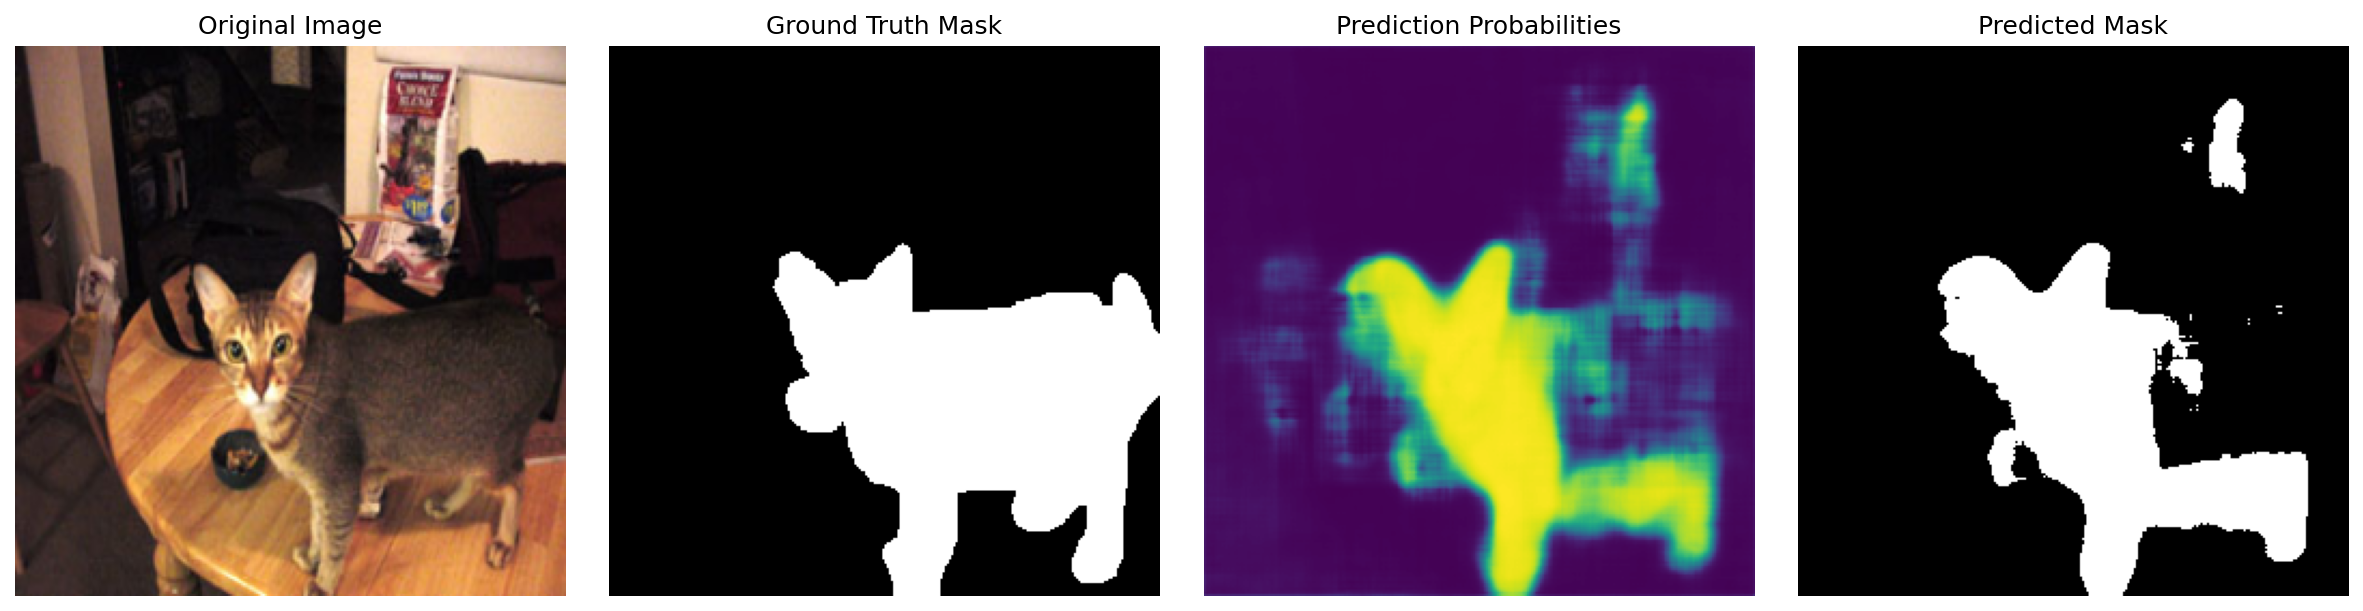
\includegraphics[width=0.95\linewidth]{figs/unet_sample_0_0}
\caption{\textbf{U-Net segmentation example 1.} From left to right: original image, ground truth mask, prediction probability map, and binary prediction mask. The U-Net accurately captures the cat's outline with high confidence.}
\label{fig:unetsample00}
\end{figure}
\begin{figure}[H]
\centering
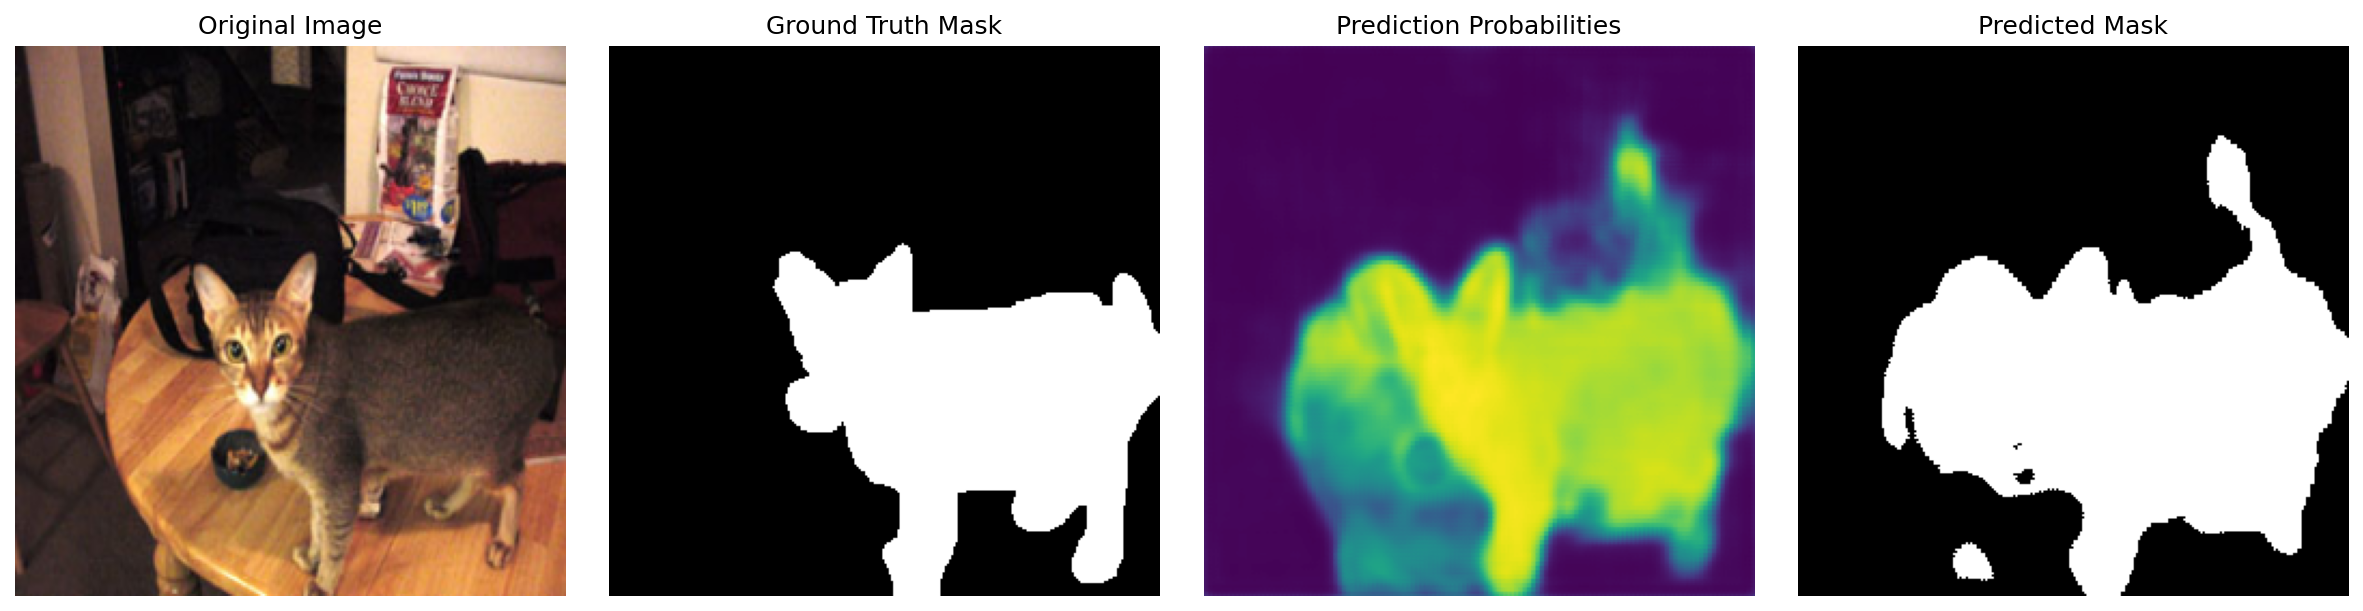
\includegraphics[width=0.95\linewidth]{figs/resnet_sample_0_0}
\caption{\textbf{ResNet34\_U-Net segmentation example 1.} From left to right: original image, ground truth mask, prediction probability map, and binary prediction mask. The ResNet34\_U-Net produces similar results to U-Net for this clear example.}
\label{fig:resnetsample00}
\end{figure}
\begin{figure}[H]
\centering
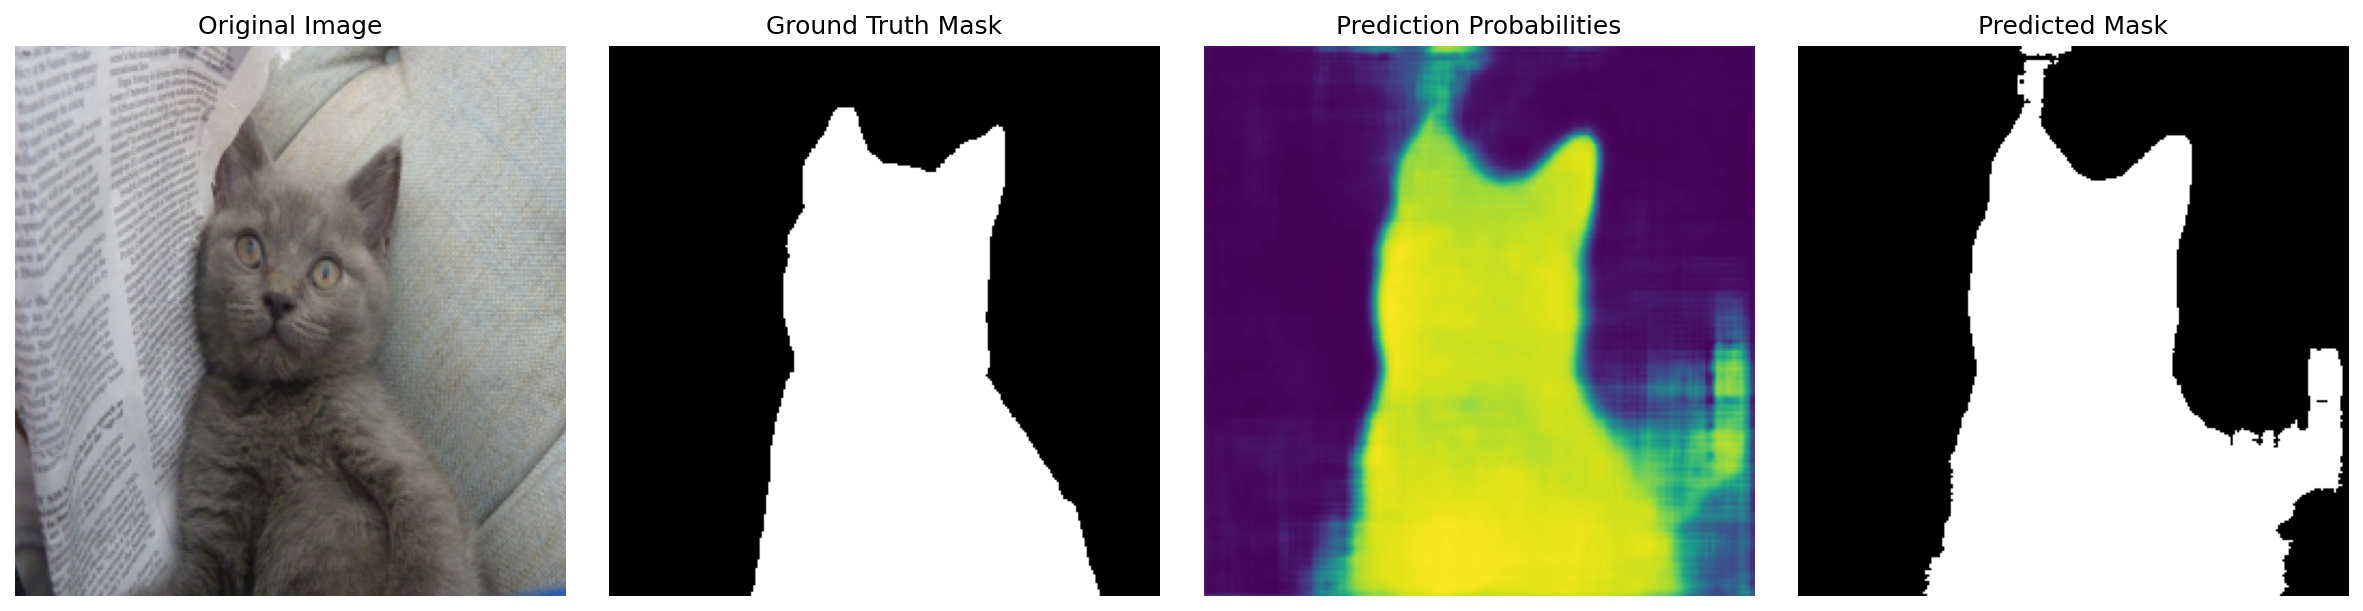
\includegraphics[width=0.95\linewidth]{figs/unet_sample_60_2}
\caption{\textbf{U-Net segmentation example 2.} From left to right: original image, ground truth mask, prediction probability map, and binary prediction mask. The U-Net successfully segments the dog despite the challenging lighting conditions and complex pose.}
\label{fig:unetsample602}
\end{figure}
\begin{figure}[H]
\centering
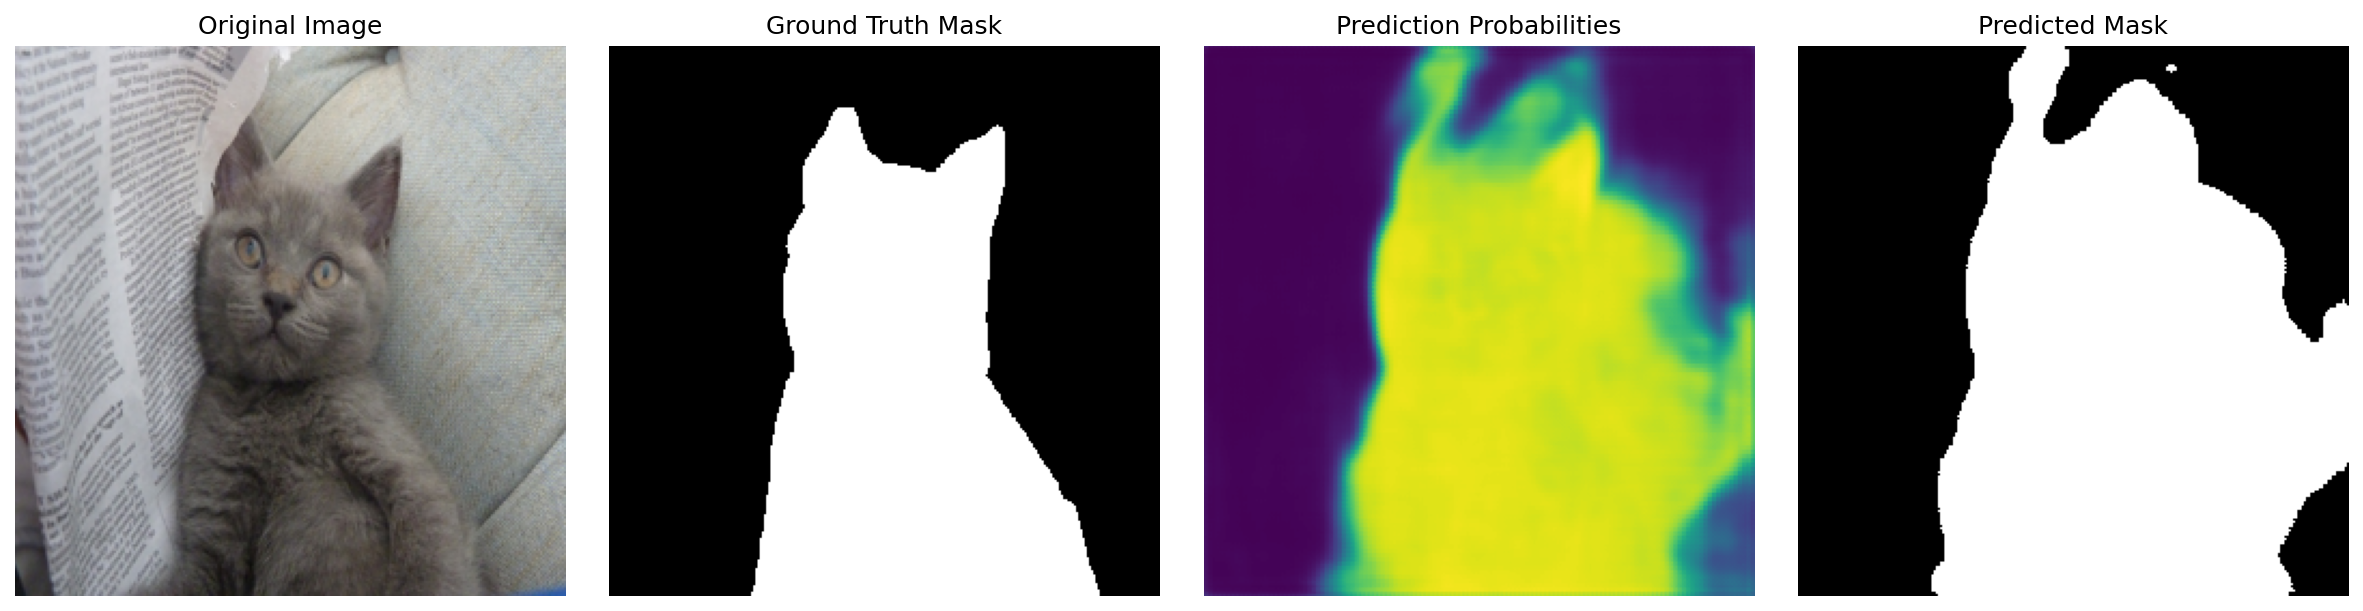
\includegraphics[width=0.95\linewidth]{figs/resnet_sample_60_2}
\caption{\textbf{ResNet34\_U-Net segmentation example 2.} From left to right: original image, ground truth mask, prediction probability map, and binary prediction mask. The ResNet34\_U-Net shows slightly less precise boundary delineation compared to U-Net for this example.}
\label{fig:resnetsample602}
\end{figure}
\begin{figure}[H]
\centering
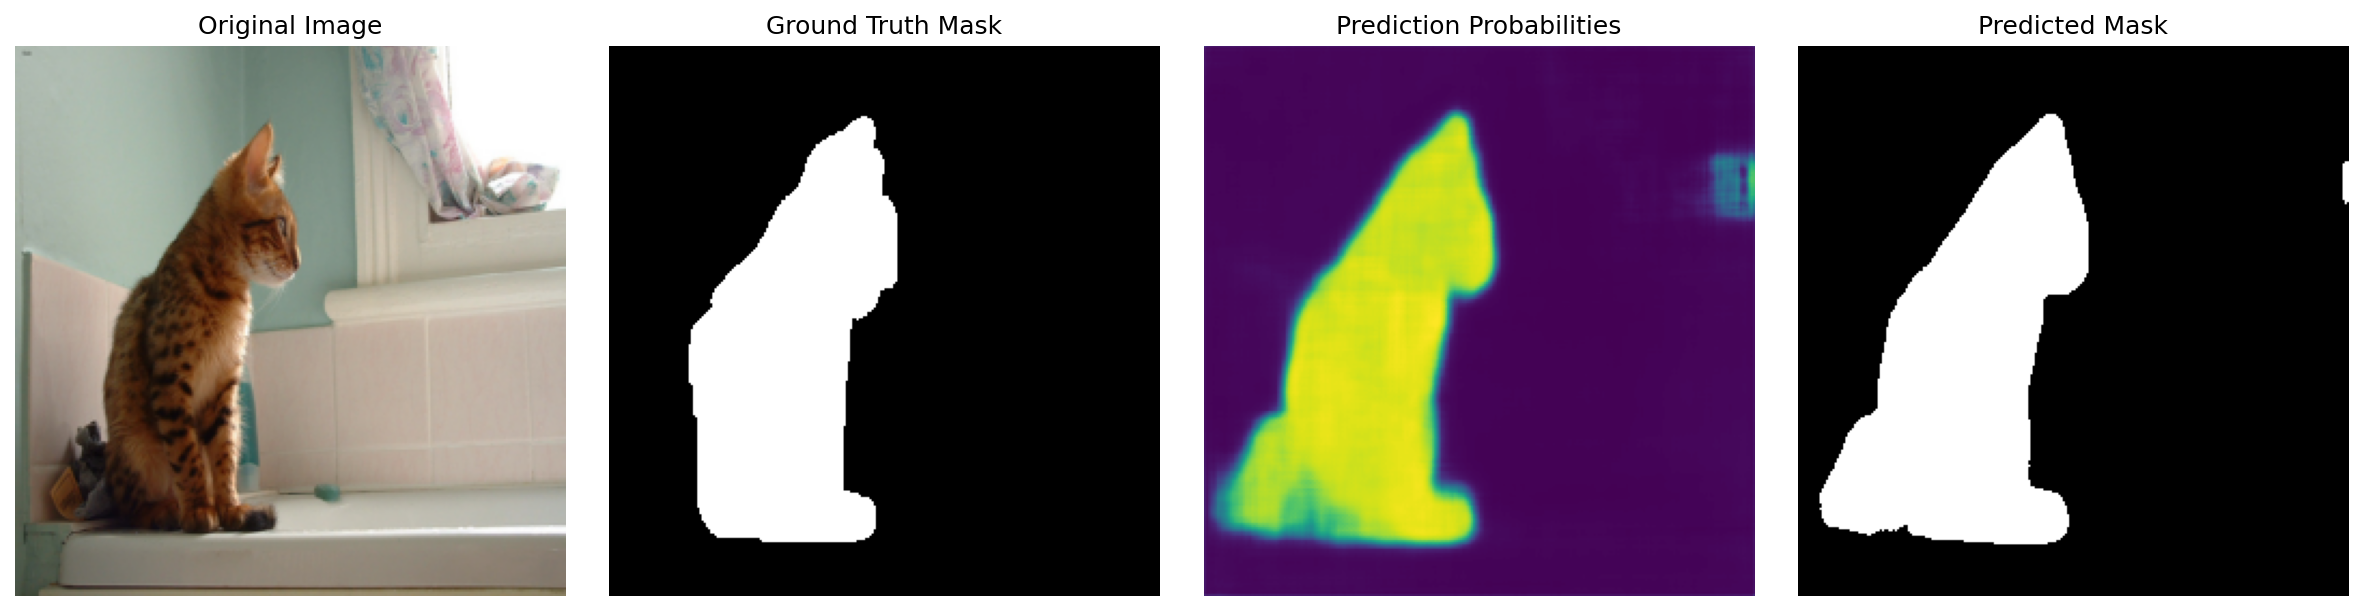
\includegraphics[width=0.95\linewidth]{figs/unet_sample_35_0}
\caption{\textbf{U-Net segmentation example 3.} From left to right: original image, ground truth mask, prediction probability map, and binary prediction mask. The U-Net correctly identifies the cat and produces a clean segmentation mask.}
\label{fig:unetsample350}
\end{figure}
\begin{figure}[H]
\centering
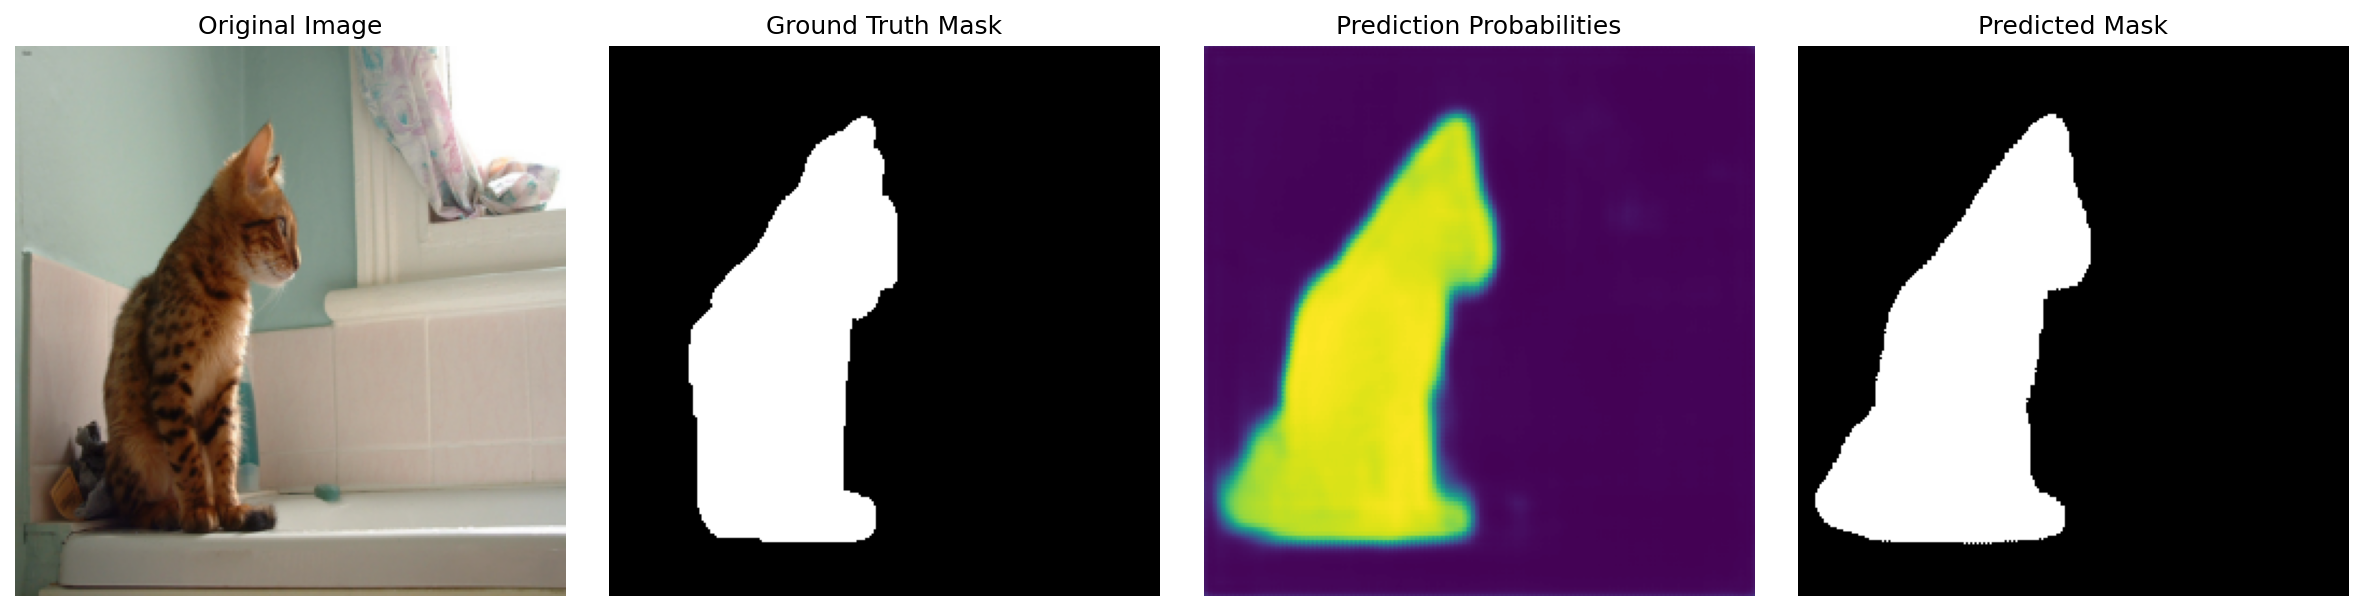
\includegraphics[width=0.95\linewidth]{figs/resnet_sample_35_0}
\caption{\textbf{ResNet34\_U-Net segmentation example 3.} From left to right: original image, ground truth mask, prediction probability map, and binary prediction mask. The ResNet34\_U-Net generates a more fragmented probability map with less confidence at the boundaries.}
\label{fig:resnetsample350}
\end{figure}

These visual examples illustrate the performance differences between the two architectures. While both models perform well on clear, well-defined images (as shown in Figures \ref{fig:unetsample350} and \ref{fig:resnetsample350}), the U-Net tends to produce more precise boundary segmentation with higher confidence at the object edges.

In the more challenging cases (Figures \ref{fig:unetsample602}, \ref{fig:resnetsample602}, \ref{fig:unetsample00}, and \ref{fig:resnetsample00}), the U-Net's probability maps show stronger boundary definition and more consistent confidence across the pet's body. The ResNet34\_U-Net's segmentations, while generally accurate, often display more uncertainty at object boundaries and occasionally produce more fragmented probability maps.

These visual results align with the quantitative findings, where U-Net achieved higher Dice scores and lower standard deviation. The examples suggest that U-Net's architecture, with its direct skip connections and gradual spatial dimension reduction, better preserves the fine-grained spatial information necessary for precise boundary delineation in semantic segmentation tasks. The ResNet34\_U-Net, while computationally more efficient, appears to sacrifice some precision in boundary detection, likely due to the more aggressive downsampling in its encoder path.

\section{Execution steps}

Please execute all scripts from the root directory.

\subsection{Training}

\begin{code}
\captionof{listing}{\textbf{The training commands.}}
\begin{minted}
python train.py --data\_path ./dataset/oxford-iiit-pet --epochs 50 --scheduler onecycle --model unet --batch\_size 32 --learning-rate 0.001  # for training unet

python train.py --data\_path ./dataset/oxford-iiit-pet --epochs 50 --scheduler onecycle --model resnet34\_unet --batch\_size 128 --learning-rate 0.001  # for training resnet34-unet
\end{minted}
\end{code}



\subsection{Evaluation}

\begin{code}
\captionof{listing}{\textbf{The evaluation commands.}}
\begin{minted}
python src/evaluate.py --model saved_models/unet_final.pth --data_path dataset/oxford-iiit-pet/ --model_type unet   # for evalauting unet

python src/evaluate.py --model saved_models/resnet34_unet_final.pth --data_path dataset/oxford-iiit-pet/ --model_type resnet34_unet  # for evalauting resnet34-unet
\end{minted}
\end{code}


\subsection{Inference}
\begin{code}
\captionof{listing}{\textbf{The inference commands.}}
\begin{minted}
python src/inference.py --model saved_models/unet_final.pth --data_path <image folder path> --model_type unet

python src/inference.py --model saved_models/resnet34_unet_final.pth --data_path <image folder path> --model_type resnet34_unet
\end{minted}
\end{code}

\section{Discussion} \label{sec:discussion}


\end{document}